\documentclass[a4paper,12pt]{article}
\usepackage{graphicx}
\usepackage{amsmath}
\usepackage{siunitx}
\sisetup{per-mode=symbol,exponent-product=\cdot,range-phrase=\ldots}
\usepackage{tikz,pgfplots}
\pgfplotsset{compat=1.18}
\usepackage{titlesec}
\usepackage{enumitem}
\usepackage{tex/ET_Ueb_Header_2Ebenen}
\graphicspath{{./}{./templates/}{./fig/}}
\renewcommand\thesection{\Alph{section}}
\titleformat{\section}[hang]{\normalfont\Large\bfseries}{Aufgabe \thesection)}{.8em}{}
\renewcommand\thesubsection{\thesection.\arabic{subsection}}
\titleformat{\subsection}[hang]{\normalfont\large\bfseries}{\thesubsection}{.8em}{}
\setlist[enumerate,1]{label=\thesubsection),ref=\thesubsection)}
\let\cpx\underline
\let\peak\hat
\newcommand\pcpx[1]{\peak{\cpx{#1}}}
\let\avg\overline
\newcommand{\abs}[1]{\left\lvert#1\right\rvert}
\newcommand{\dd}{\;\mathrm{d}}
\renewcommand{\d}{\operatorname{d}\!}
\renewcommand{\j}{\operatorname{j}\!}
\newcommand{\conj}[1]{{#1}^\ast}
\newcommand{\mat}[1]{\mathbf{#1}}
\newcommand{\cmat}[1]{\mat{\cpx{#1}}}
\makeatletter
\@ifundefined{Header}{\let\Header\makeheader}{}
\makeatother
\begin{document}
\begin{titlepage}
\thispagestyle{firstpage}
\vspace*{4cm}
\begin{center}
{\Large\bfseries Netzwerke und Schaltungen II, D-ITET\par}
\vspace{3mm}
{\Huge\bfseries Bodeplots — Musterlösung\par}
\vspace{9mm}
\end{center}
\vfill
\end{titlepage}
\section{}
\[
H(s)=\frac{1}{s+1}\,.
\]
\subsection{Bode-Diagramm}
\begin{center}
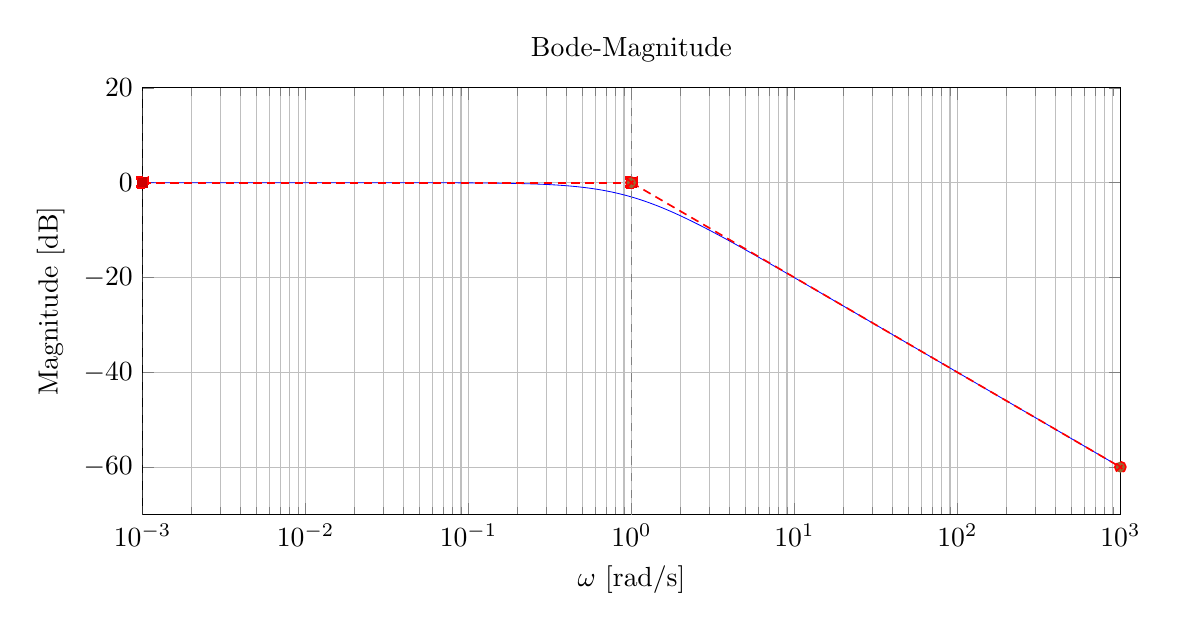
\begin{tikzpicture}
\begin{semilogxaxis}[
  width=14cm,height=7cm,
  ymin=-70,ymax=20,
  xmin=1e-3,xmax=1e3,
  xlabel={$\omega$ [rad/s]},
  ylabel={Magnitude [dB]},
  grid=both,
  title={Bode-Magnitude}
]
\addplot[
  domain=1e-3:1e3,
  samples=600,
  mark=none,
  line width=0.3pt,
  blue
] {-20*ln(sqrt(1 + x^2))/ln(10)};
\addplot+[domain=1e-3:1,samples=2,dashed,dash pattern=on 3pt off 2pt,line width=0.6pt,red] {0};
\addplot+[domain=1:1e3,samples=2,dashed,dash pattern=on 3pt off 2pt,line width=0.6pt,red] {-20*ln(x)/ln(10)};
\draw[gray,dashed] (rel axis cs:0,0) -- (rel axis cs:0,1);
\draw[gray,dashed] (axis cs:1,\pgfkeysvalueof{/pgfplots/ymin}) -- (axis cs:1,\pgfkeysvalueof{/pgfplots/ymax});
\node[gray,anchor=south east] at (axis cs:1,\pgfkeysvalueof{/pgfplots/ymax}) {\scriptsize Pol $\omega_p=1$};
\end{semilogxaxis}
\end{tikzpicture}
\vspace{6mm}
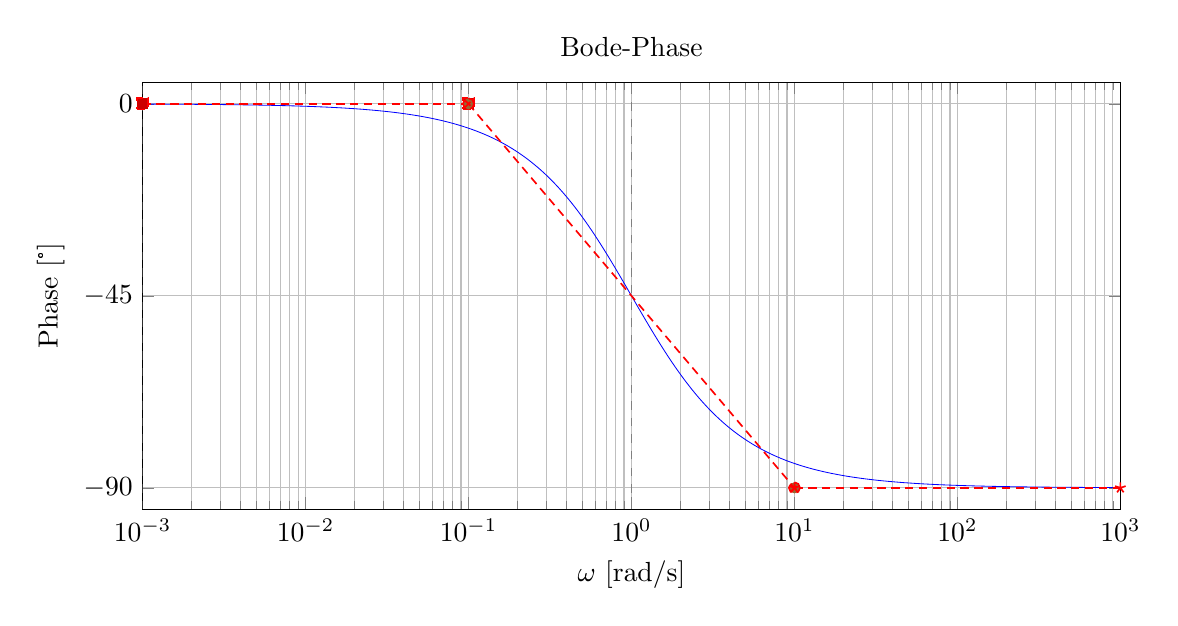
\begin{tikzpicture}
\begin{semilogxaxis}[
  width=14cm,height=7cm,
  xmin=1e-3,xmax=1e3,
  ymin=-95,ymax=5,
  ytick distance=45,
  xlabel={$\omega$ [rad/s]},
  ylabel={Phase [°]},
  grid=both,
  title={Bode-Phase}
]
\addplot[
  domain=1e-3:1e3,
  samples=600,
  mark=none,
  line width=0.3pt,
  blue
] {-atan(x)};
\addplot+[domain=1e-3:1e-1,samples=2,dashed,dash pattern=on 3pt off 2pt,line width=0.6pt,red] {0};
\addplot+[domain=1e-1:1e1,samples=2,dashed,dash pattern=on 3pt off 2pt,line width=0.6pt,red] {-45 - 45*ln(x)/ln(10)};
\addplot+[domain=1e1:1e3,samples=2,dashed,dash pattern=on 3pt off 2pt,line width=0.6pt,red] {-90};
\draw[gray,dashed] (rel axis cs:0,0) -- (rel axis cs:0,1);
\draw[gray,dashed] (axis cs:1,\pgfkeysvalueof{/pgfplots/ymin}) -- (axis cs:1,\pgfkeysvalueof{/pgfplots/ymax});
\node[gray,anchor=south east] at (axis cs:1,\pgfkeysvalueof{/pgfplots/ymax}) {\scriptsize Pol $\omega_p=1$};
\end{semilogxaxis}
\end{tikzpicture}
\end{center}

\subsection{Erklärung}
\begin{description}[leftmargin=1.2em,labelsep=.6em,font=\bfseries]

\item[1. Normalform herstellen.]
Bringe die Übertragungsfunktion exakt in die im Skript definierte Standardform für reelle Pol-/Nullstellen.
\[
H(s)=\frac{1}{1+sT_p}\quad\text{mit}\quad T_p=1.
\]
Hier haben wir: \[
\underline{F}_1(s)=\frac{1}{1+sT_p}\quad\text{und}\quad K_0 = 1\quad \text{und}\quad r = 0.
\]
Klassifizikation des ersten Teilglieds $\underline{F}_1$: reelles Polglied erster Ordnung.

\item[2. Eckfrequenz bestimmen und sortieren.]
Bestimme die Eckfrequenz aus der Zeitkonstante:
\[
\omega_p=\frac{1}{T_p}=1\,\mathrm{rad/s}.
\]
Es existiert nur diese Eckfrequenz; die aufsteigende Sortierung \(\omega_1<\omega_2<\dots\) ist damit trivial. 

\item[3. Startpunkt des Amplitudengangs festlegen (Geradennäherung).]
Setze die Startfrequenz gleich der kleinsten Eckfrequenz \(\omega_{\min}=\omega_p = 1\,\mathrm{rad/s}\). Verwende die Skript-Regel
\[
F_{\mathrm{dB}}(\omega_{\min})=20\log_{10}\!\Big(|K_0\,F^*_{ges}(0)|\cdot\,\omega_{\min}^{\,r}\Big) = 20 \log_{10}(1) = 0\,\mathrm{dB}
\]
Hier gilt \(K_0=1\), \(r=0\) und \(F^*_{ges}(0)=1\Rightarrow F_{\mathrm{dB}}(\omega_{\min})=0\,\mathrm{dB}\). Dieser Punkt nützt uns als Anker für die Geradennäherung. 

\item[4. Verlauf links vom Startpunkt zeichnen.]
Für \(\omega<\omega_{\min}\) bleibt die Amplituden-Asymptote waagrecht, denn die Anfangssteigung beträgt \(r\cdot 20\,\mathrm{dB/dec}=0\). Trage also eine horizontale Linie bei \(0\,\mathrm{dB}\) ein. 

\item[5. Steigungswechsel an der Eckfrequenz eintragen.]
Ein einfaches Polglied \(1/(1+sT_p)\) reduziert die Steigung ab \(\omega_p\) um \(20\,\mathrm{dB/dec}\). Da bist jetzt die Steigung \(0\,\mathrm{dB/dec}\) betrug, ist diese ab jetzt \(-20\,\mathrm{dB/dec}\). Zeichne rechts von \(\omega_p\) die Gerade mit Steigung \(-20\,\mathrm{dB/dec}\). Die Formel für die Geradennäherung lautet:
\[
|H(j\omega)|_{\mathrm{dB}}\approx -20\log_{10}\omega\quad(\omega\ge 1).
\]
Mehrfachpole würden die Änderung mehrfach zählen; hier nicht nötig. 

\item[6. Eckabrundung korrekt berücksichtigen.]
Bei einfachen reellen Polen ergibt sich am Knickpunkt \(\omega=\omega_p\) eine Abweichung von \(-3\,\mathrm{dB}\) gegenüber der Gerade. Setze dort einen Stützpunkt:
\[
|H(j\omega_p)|_{\mathrm{dB}}=-10\log_{10}(1+1^2)=-10\log_{10}2\approx -3.01\,\mathrm{dB}.
\]
Runde die Ecke entsprechend ab. Hätten wir einen Mehrfachpol bei \(\omega_p\) (Beispielsweise \(\big(\frac{1}{1+sT_p}\big)^t\)), müsste man die Ecke um \(t \cdot 3.01\, \mathrm{dB}\) abrunden.  

\item[7. Phasenstartwert festlegen.]
Nutze die Regel für \(\omega\to 0\): Da \(K_0F_{ges}(0)>0\) und \(r=0\), ist der Startwert der Phase
\[
\varphi(0)=0^\circ.
\]


\item[8. Phasenänderung durch das Polglied eintragen.]
Ein reelles Polglied erster Ordnung erzeugt insgesamt eine Phasenänderung von \(-90^\circ\). Trage die Näherung ein:
\[
\varphi(\omega)\approx
\begin{cases}
0^\circ,& \omega\le 0.1\,\omega_p,\\
\text{linear mit Steigung }-45^\circ/\text{Dec},& 0.1\,\omega_p<\omega<10\,\omega_p,\\
-90^\circ,& \omega\ge 10\,\omega_p.
\end{cases}
\]
Das lineare Zwischenstück kann Formelkonform als \(\varphi(\omega)\approx -45^\circ-45^\circ\log_{10}\omega\) dargestellt werden (hier mit \(\omega_p=1\)). 

\item[9. Grenzwerte und Konsistenz prüfen.]
DC: \(|H(0)|=1\Rightarrow 0\,\mathrm{dB}\), \(\varphi(0)=0^\circ\). HF: \(|H(j\omega)|\sim 1/\omega\Rightarrow -20\log_{10}\omega\,\mathrm{dB}\)). Pol-/Nullzählung bestätigt die Endphase: Zählergrad \(m=0\), Nennergra \(n=1\Rightarrow \varphi(\infty)=(m-n)\cdot 90^\circ=-90^\circ\). 

\end{description}

\subsubsection*{Stückweise Näherungen (für die Skizze)}
\[
|H(j\omega)|_{\mathrm{dB}}\approx
\begin{cases}
0,& \omega\ll 1,\\[2pt]
-10\log_{10}2,& \omega=1,\\[2pt]
-20\log_{10}\omega,& \omega\gg 1,
\end{cases}
\qquad
\varphi(\omega)\approx
\begin{cases}
0^\circ,& \omega\le 0.1,\\[2pt]
-45^\circ-45^\circ\log_{10}\omega,& 0.1<\omega<10,\\[2pt]
-90^\circ,& \omega\ge 10.
\end{cases}
\]

\newpage 
\section{}
\[
H(s)=\frac{10}{s+10}\,.
\]
\subsection{Bode-Diagramm}
\begin{center}
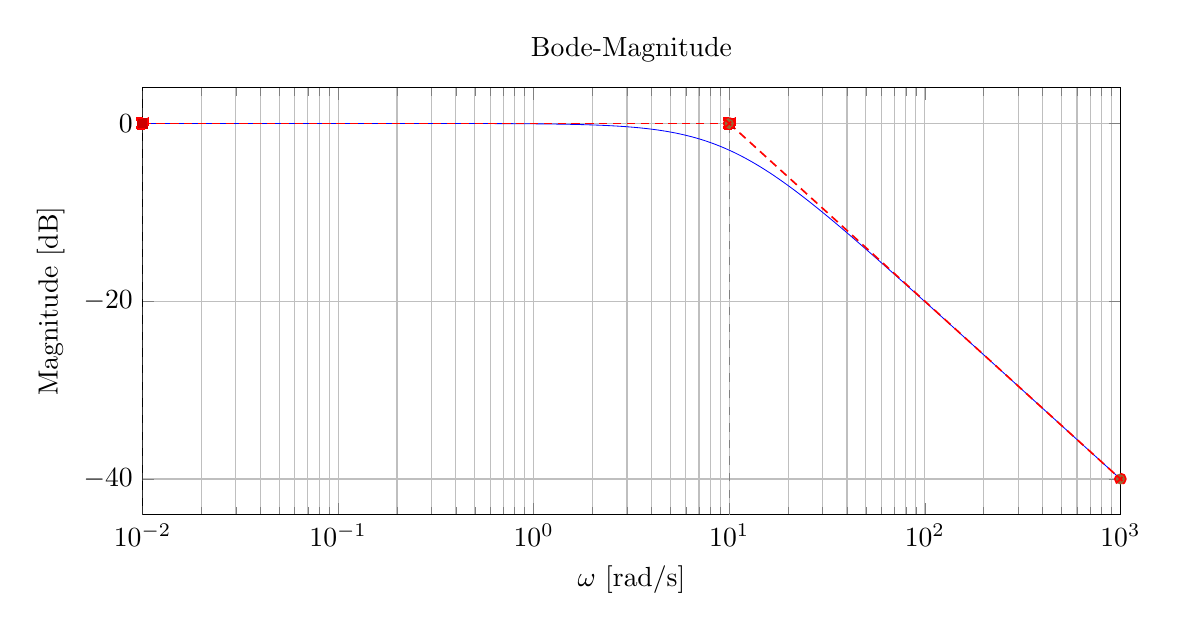
\begin{tikzpicture}
\begin{semilogxaxis}[
  width=14cm,height=7cm,
  xmin=1e-2,xmax=1e3,
  xlabel={$\omega$ [rad/s]},
  ylabel={Magnitude [dB]},
  grid=both,
  ytick distance=20, 
  title={Bode-Magnitude}
]
\addplot[
  domain=1e-2:1e3,
  samples=600,
  mark=none,
  line width=0.3pt,
  blue
] {-20*ln(sqrt(1 + (x/10)^2))/ln(10)};
\addplot+[domain=1e-2:1e1,samples=2,dashed,dash pattern=on 3pt off 2pt,line width=0.6pt,red] {0};
\addplot+[domain=1e1:1e3,samples=2,dashed,dash pattern=on 3pt off 2pt,line width=0.6pt,red] {-20*ln(x/10)/ln(10)};
\draw[gray,dashed] (rel axis cs:0,0) -- (rel axis cs:0,1);
\draw[gray,dashed] (axis cs:10,\pgfkeysvalueof{/pgfplots/ymin}) -- (axis cs:10,\pgfkeysvalueof{/pgfplots/ymax});
\node[gray,anchor=south east] at (axis cs:10,\pgfkeysvalueof{/pgfplots/ymax}) {\scriptsize Pol $\omega_p=10$};
\end{semilogxaxis}
\end{tikzpicture}
\vspace{6mm}
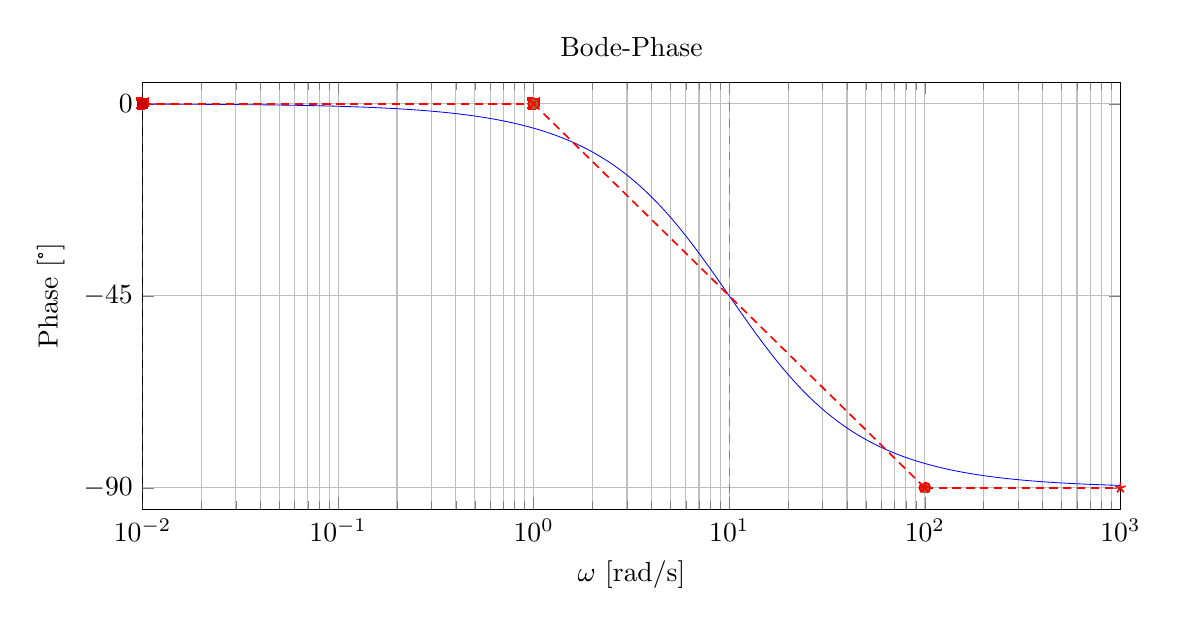
\begin{tikzpicture}
\begin{semilogxaxis}[
  width=14cm,height=7cm,
  xmin=1e-2,xmax=1e3,
  ytick distance=45,
  ymin=-95,ymax=5,
  xlabel={$\omega$ [rad/s]},
  ylabel={Phase [°]},
  grid=both,
  title={Bode-Phase}
]
\addplot[
  domain=1e-2:1e3,
  samples=600,
  mark=none,
  line width=0.3pt,
  blue
] {-atan(x/10)};
\addplot+[domain=1e-2:1e0,samples=2,dashed,dash pattern=on 3pt off 2pt,line width=0.6pt,red] {0};
\addplot+[domain=1e0:1e2,samples=2,dashed,dash pattern=on 3pt off 2pt,line width=0.6pt,red] {-45 - 45*ln(x/10)/ln(10)};
\addplot+[domain=1e2:1e3,samples=2,dashed,dash pattern=on 3pt off 2pt,line width=0.6pt,red] {-90};
\draw[gray,dashed] (rel axis cs:0,0) -- (rel axis cs:0,1);
\draw[gray,dashed] (axis cs:10,\pgfkeysvalueof{/pgfplots/ymin}) -- (axis cs:10,\pgfkeysvalueof{/pgfplots/ymax});
\node[gray,anchor=south east] at (axis cs:10,\pgfkeysvalueof{/pgfplots/ymax}) {\scriptsize Pol $\omega_p=10$};
\end{semilogxaxis}
\end{tikzpicture}
\end{center}
\newpage
\subsection{Erklärung (ausführlich)}
\begin{description}[leftmargin=1.2em,labelsep=.6em,font=\bfseries]

\item[1. Normalform herstellen.]
Bringe die Übertragungsfunktion exakt in die im Skript definierte Standardform für reelle Pol-/Nullstellen.
\[
H(s)=\frac{1}{1+sT_p}\quad\text{mit}\quad T_p=\frac{1}{10}.
\]
Hier haben wir: \[
\underline{F}_1(s)=\frac{1}{1+sT_p}\quad\text{und}\quad K_0 = 1\quad \text{und}\quad r = 0.
\]
Klassifizikation des ersten Teilglieds $\underline{F}_1$: reelles Polglied (LHP) erster Ordnung.

\item[2. Eckfrequenz bestimmen und sortieren.]
Bestimme die Eckfrequenz aus der Zeitkonstante:
\[
\omega_p=\frac{1}{T_p}=10\,\mathrm{rad/s}.
\]
Es existiert nur diese Eckfrequenz; die aufsteigende Sortierung \(\omega_1<\omega_2<\dots\) ist damit trivial. 

\item[3. Startpunkt des Amplitudengangs festlegen (Geradennäherung).]
Setze die Startfrequenz gleich der kleinsten Eckfrequenz \(\omega_{\min}=\omega_p = 10\,\mathrm{rad/s}\). Verwende die Skript-Regel
\[
F_{\mathrm{dB}}(\omega_{\min})=20\log_{10}\!\Big(|K_0\,F^*_{ges}(0)|\cdot\,\omega_{\min}^{\,r}\Big) = 20 \log_{10}(1) = 0\,\mathrm{dB}.
\]
Hier gilt \(K_0=1\), \(r=0\) und \(F^*_{ges}(0)=1\Rightarrow F_{\mathrm{dB}}(\omega_{\min})=0\,\mathrm{dB}\). Dieser Punkt nützt uns als Anker für die Geradennäherung. 

\item[4. Verlauf links vom Startpunkt zeichnen.]
Für \(\omega<\omega_{\min}\) bleibt die Amplituden-Asymptote waagrecht, denn die Anfangssteigung beträgt \(r\cdot 20\,\mathrm{dB/dec}=0\). Trage also eine horizontale Linie bei \(0\,\mathrm{dB}\) ein. 

\item[5. Steigungswechsel an der Eckfrequenz eintragen.]
Ein einfaches Polglied \(1/(1+sT_p)\) reduziert die Steigung ab \(\omega_p\) um \(20\,\mathrm{dB/dec}\). Da bis jetzt die Steigung \(0\,\mathrm{dB/dec}\) betrug, ist diese ab jetzt \(-20\,\mathrm{dB/dec}\). Zeichne rechts von \(\omega_p\) die Gerade mit Steigung \(-20\,\mathrm{dB/dec}\). Die Formel für die Geradennäherung lautet:
\[
|H(j\omega)|_{\mathrm{dB}}\approx -20\log_{10}\!\Big(\frac{\omega}{10}\Big)\quad(\omega\ge 10).
\]
Mehrfachpole würden die Änderung mehrfach zählen; hier nicht nötig. 

\item[6. Eckabrundung korrekt berücksichtigen.]
Bei einfachen reellen Polen ergibt sich am Knickpunkt \(\omega=\omega_p\) eine Abweichung von \(-3\,\mathrm{dB}\) gegenüber der Gerade.
\item[7. Phasenstartwert festlegen.]
Nutze die Regel für \(\omega\to 0\): Da \(K_0F_{ges}(0)>0\) und \(r=0\), ist der Startwert der Phase
\[
\varphi(0)=r \cdot 90^\circ=0^\circ.
\]

\item[8. Phasenänderung durch das Polglied eintragen.]
Ein reelles Polglied erster Ordnung erzeugt insgesamt eine Phasenänderung von \(-90^\circ\). Trage die Näherung ein:
\[
\varphi(\omega)\approx
\begin{cases}
0^\circ,& \omega\le 0.1\,\omega_p\;(=1),\\
\text{linear mit Steigung }-45^\circ/\text{Dec},& 0.1\,\omega_p<\omega<10\,\omega_p\;(=100),\\
-90^\circ,& \omega\ge 10\,\omega_p\;(=100).
\end{cases}
\]
Das lineare Zwischenstück kann Formelkonform als \(\varphi(\omega)\approx -45^\circ-45^\circ\log_{10}(\omega/10)\) dargestellt werden (hier mit \(\omega_p=10\)). 

\item[9. Grenzwerte und Konsistenz prüfen.]
DC: \(|H(0)|=1\Rightarrow 0\,\mathrm{dB}\), \(\varphi(0)=0^\circ\). HF: \(|H(j\omega)|\sim 10/\omega\Rightarrow -20\log_{10}(\omega/10)\,\mathrm{dB}\)). Pol-/Nullzählung bestätigt die Endphase: Zählergrad \(m=0\), Nennergrad \(n=1\Rightarrow \varphi(\infty)=(m-n)\cdot 90^\circ=-90^\circ\). 

\end{description}

\subsubsection*{Stückweise Näherungen (für die Skizze)}
\[
|H(j\omega)|_{\mathrm{dB}}\approx
\begin{cases}
0,& \omega\ll 10,\\[2pt]
-10\log_{10}2,& \omega=10,\\[2pt]
-20\log_{10}(\omega/10),& \omega\gg 10,
\end{cases}
\]
\vspace{0.3cm}
\[
\varphi(\omega)\approx
\begin{cases}
0^\circ,& \omega\le 1,\\[2pt]
-45^\circ-45^\circ\log_{10}(\omega/10),& 1<\omega<100,\\[2pt]
-90^\circ,& \omega\ge 100.
\end{cases}
\]

\newpage
\section{}
\[
H(s)=\frac{s+1}{s+10}\,.
\]
\subsection{Bode-Diagramm}
\begin{center}
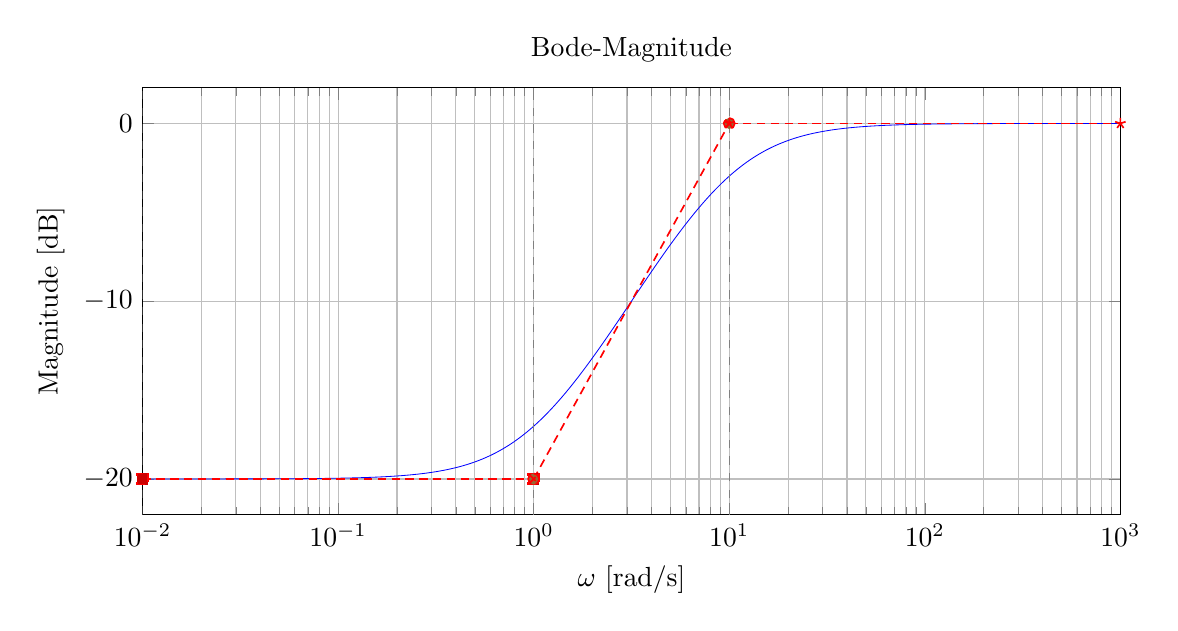
\begin{tikzpicture}
\begin{semilogxaxis}[
  width=14cm,height=7cm,
  xmin=1e-2,xmax=1e3,
  xlabel={$\omega$ [rad/s]},
  ylabel={Magnitude [dB]},
  grid=both,
  ytick distance=10,
  title={Bode-Magnitude}
]
\addplot[
  domain=1e-2:1e3,
  samples=600,
  mark=none,
  line width=0.3pt,
  blue
] {20*ln(sqrt(1 + x^2))/ln(10) - 20*ln(sqrt(100 + x^2))/ln(10)};
\addplot+[domain=1e-2:1,samples=2,dashed,dash pattern=on 3pt off 2pt,line width=0.6pt,red] {-20};
\addplot+[domain=1:1e1,samples=2,dashed,dash pattern=on 3pt off 2pt,line width=0.6pt,red] {-20 + 20*ln(x)/ln(10)};
\addplot+[domain=1e1:1e3,samples=2,dashed,dash pattern=on 3pt off 2pt,line width=0.6pt,red] {0};
\draw[gray,dashed] (rel axis cs:0,0) -- (rel axis cs:0,1);
\draw[gray,dashed] (axis cs:1,\pgfkeysvalueof{/pgfplots/ymin}) -- (axis cs:1,\pgfkeysvalueof{/pgfplots/ymax});
\draw[gray,dashed] (axis cs:10,\pgfkeysvalueof{/pgfplots/ymin}) -- (axis cs:10,\pgfkeysvalueof{/pgfplots/ymax});
\node[gray,anchor=south east] at (axis cs:1,\pgfkeysvalueof{/pgfplots/ymax}) {\scriptsize Nullstelle $\omega_z=1$};
\node[gray,anchor=south east] at (axis cs:10,\pgfkeysvalueof{/pgfplots/ymax}) {\scriptsize Pol $\omega_p=10$};
\end{semilogxaxis}
\end{tikzpicture}
\vspace{6mm}
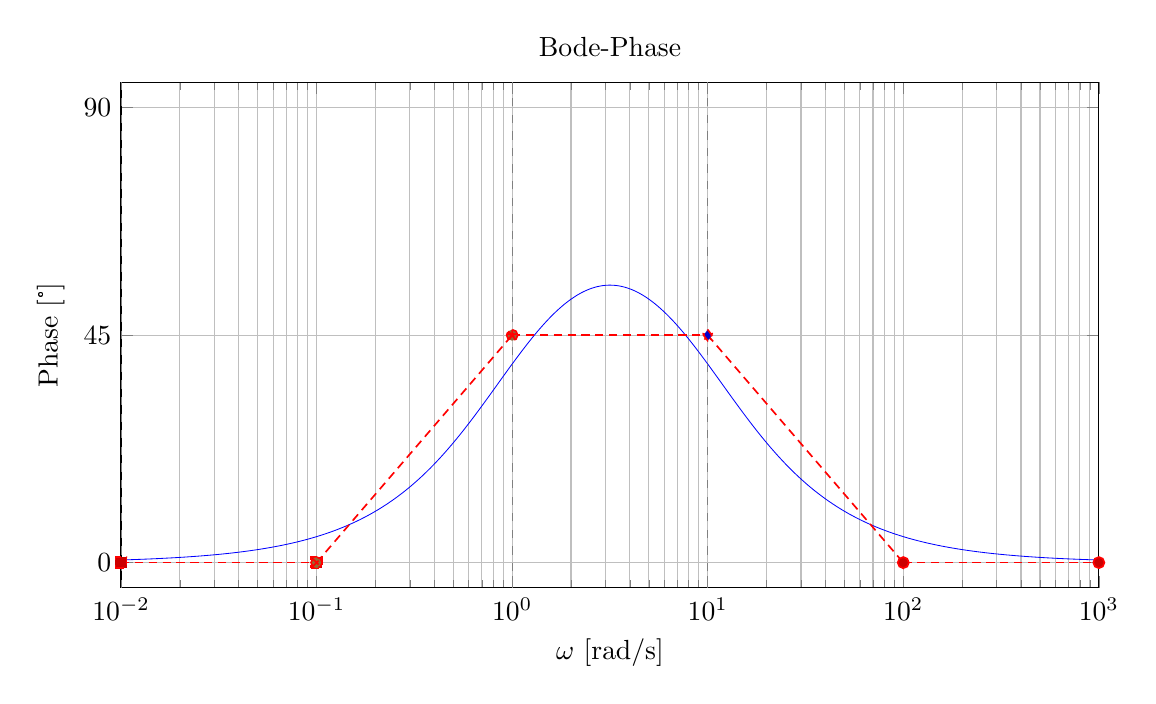
\begin{tikzpicture}
\begin{semilogxaxis}[
  width=14cm,height=8cm,
  xmin=1e-2,xmax=1e3,
  ymin=-5,ymax=95,
  ytick distance=45,
  xlabel={$\omega$ [rad/s]},
  ylabel={Phase [°]},
  grid=both,
  title={Bode-Phase}
]
\addplot[
  domain=1e-2:1e3,
  samples=600,
  mark=none,
  line width=0.3pt,
  blue
] {atan(x) - atan(x/10)};
\addplot+[domain=1e-2:1e-1,samples=2,dashed,dash pattern=on 3pt off 2pt,line width=0.6pt,red] {0};
\addplot+[domain=1e-1:1e0,samples=2,dashed,dash pattern=on 3pt off 2pt,line width=0.6pt,red] {45 + 45*ln(x)/ln(10)};
\addplot+[domain=1e0:1e1,samples=2,dashed,dash pattern=on 3pt off 2pt,line width=0.6pt,red] {45};
\addplot+[domain=1e1:1e2,samples=2,dashed,dash pattern=on 3pt off 2pt,line width=0.6pt,red] {45 - 45*ln(x/10)/ln(10)};
\addplot+[domain=1e2:1e3,samples=2,dashed,dash pattern=on 3pt off 2pt,line width=0.6pt,red] {0};
\draw[gray,dashed] (rel axis cs:0,0) -- (rel axis cs:0,1);
\draw[gray,dashed] (axis cs:1,\pgfkeysvalueof{/pgfplots/ymin}) -- (axis cs:1,\pgfkeysvalueof{/pgfplots/ymax});
\draw[gray,dashed] (axis cs:10,\pgfkeysvalueof{/pgfplots/ymin}) -- (axis cs:10,\pgfkeysvalueof{/pgfplots/ymax});
\node[gray,anchor=south east] at (axis cs:1,\pgfkeysvalueof{/pgfplots/ymax}) {\scriptsize Nullstelle $\omega_z=1$};
\node[gray,anchor=south east] at (axis cs:10,\pgfkeysvalueof{/pgfplots/ymax}) {\scriptsize Pol $\omega_p=10$};
\end{semilogxaxis}
\end{tikzpicture}
\end{center}
\newpage
\subsection{Erklärung}
\vspace{5mm}
\begin{description}[leftmargin=1.2em,labelsep=.6em,font=\bfseries]
\item[Schritt 1] DC-Faktor $\tfrac{1}{10}$: $H(s)=\tfrac{s+1}{s+10}=\tfrac{1+s}{10(1+s/10)}$. Für $\omega\ll1$ dominiert der DC-Anteil: $|H(\j\omega)|\approx\tfrac{1}{10}$, daher Betrag $-20\,\mathrm{dB}$ ohne Startsteigung; Startphase $\approx0^\circ$.
\item[Schritt 2] Nullstelle bei $\omega_z=1\,\mathrm{rad/s}$: ab $\omega=1$ steigt die Magnitude mit $+20\,\mathrm{dB/dec}$; zwischen $\omega_l=0.1$ und $\omega_h=10$ wächst die Phasenbeitrag der Nullstelle näherungsweise linear von $0^\circ$ auf $+90^\circ$ (Geradennäherung: $+45^\circ+45\log_{10}\omega$ in $[0.1,10]$), sodass bei $\omega=1$ etwa $+45^\circ$ erreicht werden.
\item[Schritt 3] Pol bei $\omega_p=10\,\mathrm{rad/s}$: ab $\omega=10$ kommt ein Steigungswechsel von $-20\,\mathrm{dB/dec}$ hinzu; dadurch wird die Gesamtslope wieder $0\,\mathrm{dB/dec}$ und der Betrag konvergiert gegen $0\,\mathrm{dB}$ für $\omega\gg10$. Der Pol führt in $[1,100]$ zu einer Phasenabnahme um $90^\circ$ (Geradennäherung: $+45^\circ-45\log_{10}(\omega/10)$), sodass die Gesamtphase für $\omega\gg100$ wieder gegen $0^\circ$ fällt. Das Zwischenband $1\le\omega\le10$ ist somit nahezu phasenflach bei $\approx+45^\circ$ und weist eine Betrags-Slope von $+20\,\mathrm{dB/dec}$ auf.
\end{description}

\vspace{0.5cm}
\medskip
\noindent\textbf{Stückweise Näherung}
\[
|H(\j\omega)|_{\mathrm{dB}}\approx
\begin{cases}
-20,& \omega\ll1,\\[4pt]
-20+20\log_{10}\omega,& 1\ll\omega\ll10,\\[4pt]
0,& \omega\gg10,
\end{cases}
\qquad
\]
\newpage
\section{}
\[
H(s)=\frac{10\,(1 - s)}{s+10}\,.
\]
\subsection{Bode-Diagramm}
\begin{center}
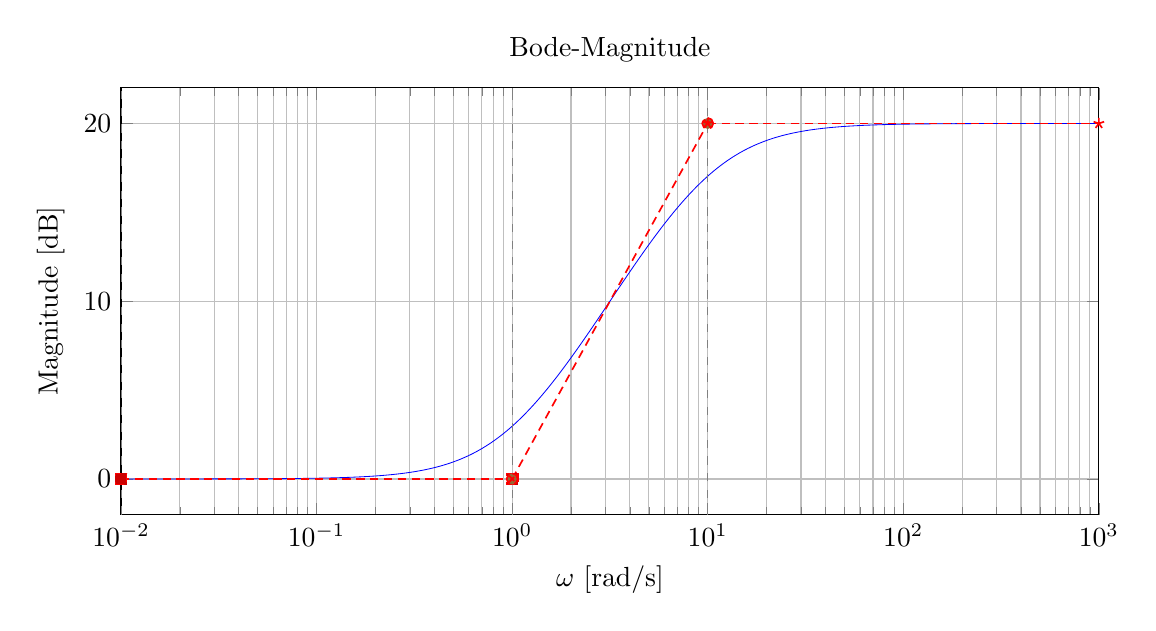
\begin{tikzpicture}
\begin{semilogxaxis}[
  width=14cm,height=7cm,
  xmin=1e-2,xmax=1e3,
  xlabel={$\omega$ [rad/s]},
  ylabel={Magnitude [dB]},
  grid=both,
  ytick distance=10,
  title={Bode-Magnitude}
]
\addplot[
  domain=1e-2:1e3,
  samples=600,
  mark=none,
  ytick distance=10,
  line width=0.3pt,
  blue
] {20 + 20*ln(sqrt(1 + x^2))/ln(10) - 20*ln(sqrt(100 + x^2))/ln(10)};
\addplot+[domain=1e-2:1,samples=2,dashed,dash pattern=on 3pt off 2pt,line width=0.6pt,red] {0};
\addplot+[domain=1:1e1,samples=2,dashed,dash pattern=on 3pt off 2pt,line width=0.6pt,red] {20*ln(x)/ln(10)};
\addplot+[domain=1e1:1e3,samples=2,dashed,dash pattern=on 3pt off 2pt,line width=0.6pt,red] {20};
\draw[gray,dashed] (rel axis cs:0,0) -- (rel axis cs:0,1);
\draw[gray,dashed] (axis cs:1,\pgfkeysvalueof{/pgfplots/ymin}) -- (axis cs:1,\pgfkeysvalueof{/pgfplots/ymax});
\draw[gray,dashed] (axis cs:10,\pgfkeysvalueof{/pgfplots/ymin}) -- (axis cs:10,\pgfkeysvalueof{/pgfplots/ymax});
\node[gray,anchor=south east] at (axis cs:1,\pgfkeysvalueof{/pgfplots/ymax}) {\scriptsize Nullstelle $\omega_z=1$ (RHP)};
\node[gray,anchor=south east] at (axis cs:10,\pgfkeysvalueof{/pgfplots/ymax}) {\scriptsize Pol $\omega_p=10$};
\end{semilogxaxis}
\end{tikzpicture}
\vspace{6mm}
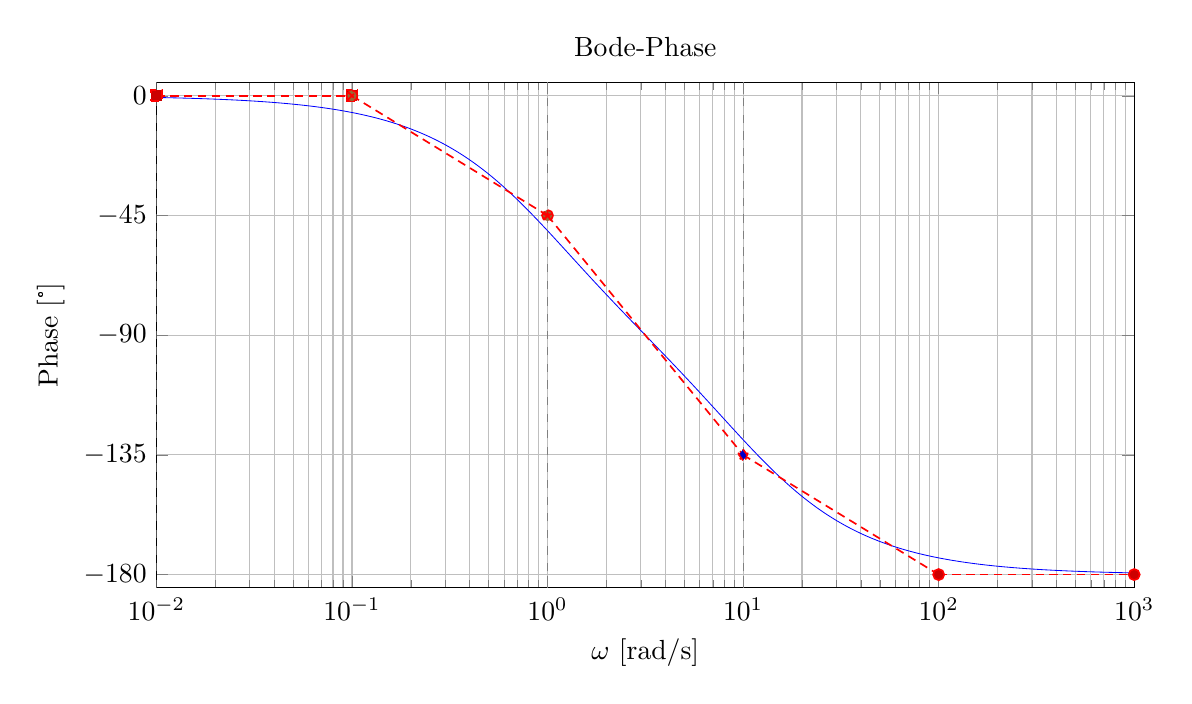
\begin{tikzpicture}
\begin{semilogxaxis}[
  width=14cm,height=8cm,
  xmin=1e-2,xmax=1e3,
  ymin=-185,ymax=5,
  xlabel={$\omega$ [rad/s]},
  ylabel={Phase [°]},
  ytick distance=45,
  grid=both,
  title={Bode-Phase}
]
\addplot[
  domain=1e-2:1e3,
  samples=600,
  mark=none,
  line width=0.3pt,
  blue
] {-atan(x) - atan(x/10)};
\addplot+[domain=1e-2:1e-1,samples=2,dashed,dash pattern=on 3pt off 2pt,line width=0.6pt,red] {0};
\addplot+[domain=1e-1:1e0,samples=2,dashed,dash pattern=on 3pt off 2pt,line width=0.6pt,red] {-45 - 45*ln(x)/ln(10)};
\addplot+[domain=1e0:1e1,samples=2,dashed,dash pattern=on 3pt off 2pt,line width=0.6pt,red]{-45 - 90*ln(x)/ln(10)};
\addplot+[domain=1e1:1e2,samples=2,dashed,dash pattern=on 3pt off 2pt,line width=0.6pt,red] {-135 - 45*ln(x/10)/ln(10)};
\addplot+[domain=1e2:1e3,samples=2,dashed,dash pattern=on 3pt off 2pt,line width=0.6pt,red] {-180};
\draw[gray,dashed] (rel axis cs:0,0) -- (rel axis cs:0,1);
\draw[gray,dashed] (axis cs:1,\pgfkeysvalueof{/pgfplots/ymin}) -- (axis cs:1,\pgfkeysvalueof{/pgfplots/ymax});
\draw[gray,dashed] (axis cs:10,\pgfkeysvalueof{/pgfplots/ymin}) -- (axis cs:10,\pgfkeysvalueof{/pgfplots/ymax});
\node[gray,anchor=south east] at (axis cs:1,\pgfkeysvalueof{/pgfplots/ymax}) {\scriptsize Nullstelle $\omega_z=1$ (RHP)};
\node[gray,anchor=south east] at (axis cs:10,\pgfkeysvalueof{/pgfplots/ymax}) {\scriptsize Pol $\omega_p=10$};
\end{semilogxaxis}
\end{tikzpicture}
\end{center}
\newpage
\subsection{Erklärung}
\begin{description}[leftmargin=1.2em,labelsep=.6em,font=\bfseries]

\item[1. Normalform herstellen.]
Bringe die Übertragungsfunktion exakt in die im Skript definierte Standardform.
\[
H(s)=\frac{10(1-s)}{s+10}
= (1 - sT_z)\cdot\frac{1}{1+sT_p}\,.
\]
mit \(K_0=1\), \(r=0\), \(T_z=1\), \(T_p=\tfrac{1}{10}\).
Klassifiziere die Glieder: RHP-Nullstelle \(\underline{F}_z(s)=(1-sT_z)\) mit \(T_z=1\); reelles Polglied \(\underline{F}_p(s)=\tfrac{1}{1+sT_p}\) mit \(T_p=\tfrac{1}{10}\).


\item[2. Eckfrequenzen bestimmen und sortieren.] Die $\omega$-Eckfrequenzen lassen sich aus den $T_n$'s bestimmen und müssen anschließend sortiert werden:
\[
\omega_z=\frac{1}{T_z}=1\,\mathrm{rad/s},\qquad \omega_p=\frac{1}{T_p}=10\,\mathrm{rad/s},\qquad \omega_z<\omega_p.
\]

\item[3. Startpunkt des Amplitudengangs festlegen (Geradennäherung).]
Wähle \(\omega_{\min}=\omega_z=1\). Regel:
\[
F_{\mathrm{dB}}(\omega_{\min})=20\log_{10}\!\big(|K_0F^*_{ges}(0)|\cdot\omega_{\min}^{\,r}\big)
=20\log_{10}(1)=0\,\mathrm{dB}.
\]
Dieser Punkt ist der Anker der Geradennäherung.

\item[4. Verlauf links vom Startpunkt zeichnen.]
Für \(\omega<\omega_z\) bleibt die Amplituden-Asymptote bei \(0\,\mathrm{dB}\) konstant (Anfangssteigung \(r\cdot 20 \,\mathrm{dB}=0\)). Zeichne eine waagrechte Gerade links von der kleinsten Eckfrequenz.

\item[5. Steigungswechsel an den Eckfrequenzen eintragen.]
Ab der RHP-Nullstelle bei \(\omega_z=1\) nimmt die Steigung um \(+20\,\mathrm{dB/dec}\) zu.
Der Pol bei \(\omega_p=10\) bewirkt einen zusätzlichen Steigungswechsel um \(-20\,\mathrm{dB/dec}\) ab \(\omega=10\).
Netto:
\[
\begin{cases}
0\,\mathrm{dB/dec},& \omega<1,\\
+20\,\mathrm{dB/dec},& 1\le\omega<10,\\
0\,\mathrm{dB/dec},& \omega\ge 10\;\Rightarrow |H|\to 20\,\mathrm{dB}.
\end{cases}
\]
Geradennäherungen:
\[
|H(j\omega)|_{\mathrm{dB}}\approx
\begin{cases}
0,& \omega\le 1,\\
20\log_{10}\omega,& 1<\omega\le 10,\\
20,& \omega\ge 10.
\end{cases}
\]

\item[6. Eckabrundungen korrekt berücksichtigen.]
RHP-Nullstelle: bei \(\omega=\omega_z\) liegt die exakte Magnitude um \(+3\,\mathrm{dB}\) über der Asymptote.
Pol: bei \(\omega=\omega_p\) liegt die exakte Magnitude um \(-3\,\mathrm{dB}\) unter der Asymptote.
Stützpunkte:
\[
|H(j1)|_{\mathrm{dB}}=20+10\log_{10}(2)-10\log_{10}(101)\approx +3\,\mathrm{dB},
\]
\[
|H(j10)|_{\mathrm{dB}}=20+10\log_{10}(101)-10\log_{10}(200)\approx 17\,\mathrm{dB}.
\]

\item[7. Phasenstartwert festlegen.]
Nutze die Regel für \(\omega\to 0\): Da \(K_0F_{ges}(0)>0\) und \(r=0\), ist der Startwert der Phase
\[
\varphi(0)=r \cdot 90^\circ=0^\circ.
\]

\item[8. Phasenänderung durch Nullstelle und Pol eintragen.]
RHP-Nullstelle bei \(\omega_z=1\): Phasenänderung \(-90^\circ\) über die Dekade \([0.1,10]\) (Geradennäherung \(-45^\circ-45^\circ\log_{10}\omega\)).
Pol bei \(\omega_p=10\): zusätzlicher Abfall um \(-90^\circ\) über \([1,100]\) (Geradennäherung \(-45^\circ-45^\circ\log_{10}(\omega/10)\)). Im Intervar $[1,10]$ überlagern sich diese Effekte.
Gesamt:
\[
\varphi(\omega)\approx
\begin{cases}
0^\circ,& \omega\le 0.1,\\
-45^\circ-45^\circ\log_{10}\omega,& 0.1<\omega\le 1,\\
-45^\circ-90^\circ\log_{10}\omega,& 1<\omega\le 10,\\
-135^\circ-45^\circ\log_{10}(\omega/10),& 10<\omega\le 100,\\
-180^\circ,& \omega\ge 100.
\end{cases}
\]

\item[9. Grenzwerte und Konsistenz prüfen.]
DC: \(|H(0)|=1\Rightarrow 0\,\mathrm{dB}\), \(\varphi(0)=0^\circ\).
HF: \(|H(j\omega)|\to 10\Rightarrow 20\,\mathrm{dB}\).
Pol-/Nullzählung bestätigt die Endphase: Zählergrad \(m=-1\), Nennergrad \(n=1\) \(\Rightarrow (m-n)\cdot 90^\circ=0^\circ\); $m=-1$, da die Nullstelle RHP ist.

\end{description}

\subsubsection*{Stückweise Näherungen (für die Skizze)}
\[
|H(j\omega)|_{\mathrm{dB}}\approx
\begin{cases}
0,& \omega\ll 1,\\[2pt]
20\log_{10}\omega,& 1\ll\omega\ll 10,\\[2pt]
20,& \omega\gg 10,
\end{cases}
\]
\[
\varphi(\omega)\approx
\begin{cases}
0^\circ,& \omega\le 0.1,\\[2pt]
-45^\circ-45^\circ\log_{10}\omega,& 0.1<\omega<1,\\[2pt]
-45^\circ-90^\circ\log_{10}\omega,& 1<\omega<10,\\[2pt]
-135^\circ-45^\circ\log_{10}(\omega/10),& 10<\omega<100,\\[2pt]
-180^\circ,& \omega\ge 100.
\end{cases}
\]

\newpage
\section{}
\[
H(s)=\frac{-1+\j}{\sqrt{2}\,(s+1)^2}\,.
\]
\subsection{Bode-Diagramm}
\begin{center}
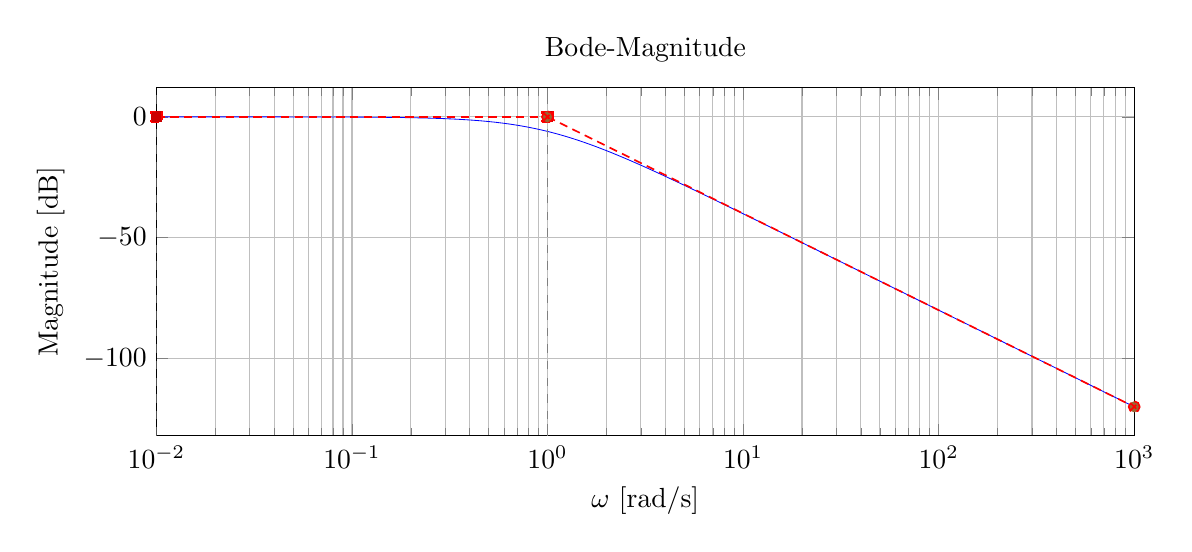
\begin{tikzpicture}
\begin{semilogxaxis}[
  width=14cm,height=6cm,
  xmin=1e-2,xmax=1e3,
  xlabel={$\omega$ [rad/s]},
  ylabel={Magnitude [dB]},
  grid=both,
  title={Bode-Magnitude}
]
\addplot[
  domain=1e-2:1e3,
  samples=600,
  mark=none,
  line width=0.3pt,
  blue
] {-40*ln(sqrt(1 + x^2))/ln(10)};
\addplot+[domain=1e-2:1,samples=2,dashed,dash pattern=on 3pt off 2pt,line width=0.6pt,red] {0};
\addplot+[domain=1:1e3,samples=2,dashed,dash pattern=on 3pt off 2pt,line width=0.6pt,red] {-40*ln(x)/ln(10)};
\draw[gray,dashed] (rel axis cs:0,0) -- (rel axis cs:0,1);
\draw[gray,dashed] (axis cs:1,\pgfkeysvalueof{/pgfplots/ymin}) -- (axis cs:1,\pgfkeysvalueof{/pgfplots/ymax});
\node[gray,anchor=south east] at (axis cs:1,\pgfkeysvalueof{/pgfplots/ymax}) {\scriptsize Pol $\omega_p=1$ (doppelt)};
\end{semilogxaxis}
\end{tikzpicture}
\vspace{6mm}
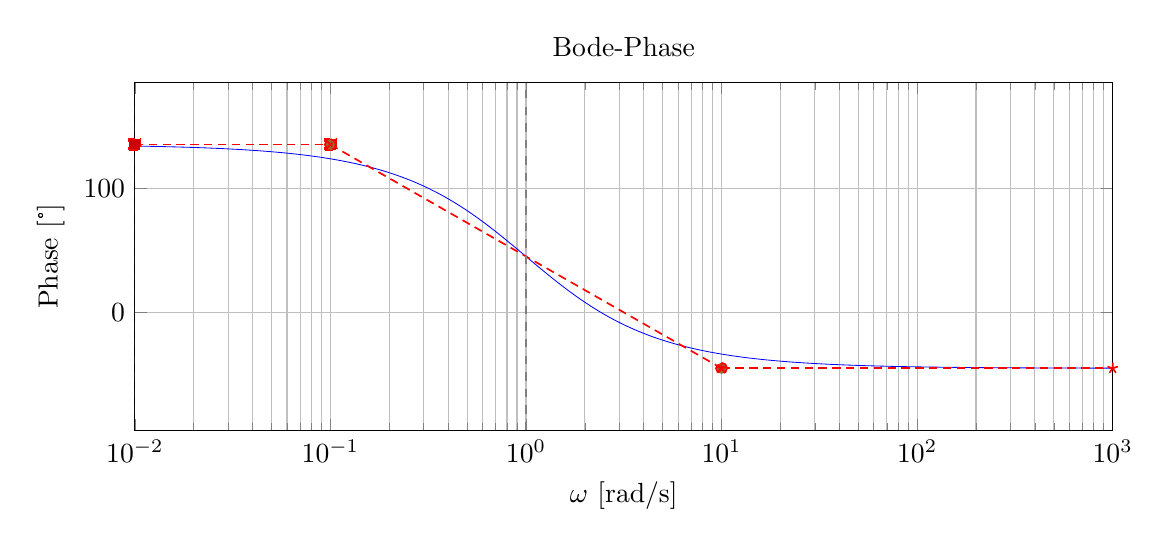
\begin{tikzpicture}
\begin{semilogxaxis}[
  width=14cm,height=6cm,
  xmin=1e-2,xmax=1e3,
  ymin=-95,ymax=185,
  xlabel={$\omega$ [rad/s]},
  ylabel={Phase [°]},
  grid=both,
  title={Bode-Phase}
]
\addplot[
  domain=1e-2:1e3,
  samples=600,
  mark=none,
  line width=0.3pt,
  blue
] {135 - 2*atan(x)};
\addplot+[domain=1e-2:1e-1,samples=2,dashed,dash pattern=on 3pt off 2pt,line width=0.6pt,red] {135};
\addplot+[domain=1e-1:1e1,samples=2,dashed,dash pattern=on 3pt off 2pt,line width=0.6pt,red] {45 - 90*ln(x)/ln(10)};
\addplot+[domain=1e1:1e3,samples=2,dashed,dash pattern=on 3pt off 2pt,line width=0.6pt,red] {-45};
\draw[gray,dashed] (rel axis cs:0,0) -- (rel axis cs:0,1);
\draw[gray,dashed] (axis cs:1,\pgfkeysvalueof{/pgfplots/ymin}) -- (axis cs:1,\pgfkeysvalueof{/pgfplots/ymax});
\node[gray,anchor=south east] at (axis cs:1,\pgfkeysvalueof{/pgfplots/ymax}) {\scriptsize Pol $\omega_p=1$ (doppelt)};
\end{semilogxaxis}
\end{tikzpicture}
\end{center}
\newpage
\subsection{Erklärung}
\vspace{5mm}
\begin{description}[leftmargin=1.2em,labelsep=.6em,font=\bfseries]
\item[Schritt 1] Konstanter Faktor $(-1+\j)/\sqrt{2}=\mathrm{e}^{\j135^\circ}$: Betrag $1\Rightarrow$ Start bei $0\,\mathrm{dB}$ ohne Anfangssteigung; die Phase ist über alle Frequenzen um $+135^\circ$ verschoben (reiner Phasor, kein Einfluss auf die Magnitude).
\item[Schritt 2] Doppelpol bei $\omega_p=1\,\mathrm{rad/s}$: ab $\omega=1$ sinkt die Magnitude mit $-40\,\mathrm{dB/dec}$; am Eckpunkt beträgt die exakte Dämpfung $-20\log_{10}(1+1)= -20\log_{10}2\approx-6.02\,\mathrm{dB}$ (Summe aus zwei $\,-3.01\,\mathrm{dB}$). Die Phase der beiden gleichliegenden Pole fällt zusammen in der Übergangsdekade $\omega\in[0.1,10]$ insgesamt um $180^\circ$; lineare Geradennäherung: $135^\circ\to-45^\circ$ mit $\;\varphi_{\text{approx}}(\omega)=45^\circ-90^\circ\log_{10}\omega$ für $\omega\in[0.1,10]$.
\item[Schritt 3] Grenzverhalten: für $\omega\ll1$ gilt $|H(\j\omega)|_{\mathrm{dB}}\approx0\,\mathrm{dB}$ und $\angle H\approx+135^\circ$; für $\omega\gg1$ folgt $|H(\j\omega)|_{\mathrm{dB}}\approx-40\log_{10}\omega$ und die Phase nähert sich $+135^\circ-2\cdot90^\circ=-45^\circ$ an.
\end{description}

\vspace{0.5cm}
\medskip
\noindent\textbf{Stückweise Näherung}
\[
|H(\j\omega)|_{\mathrm{dB}}\approx
\begin{cases}
0,& \omega\ll1,\\[4pt]
-20\log_{10}2,& \omega=1,\\[4pt]
-40\log_{10}\omega,& \omega\gg1,
\end{cases}
\qquad
\]
\newpage
\section{}
\[
H(s)=\frac{-1000}{(s+1)(s+100)}\,.
\]
\subsection{Bode-Diagramm}
\begin{center}
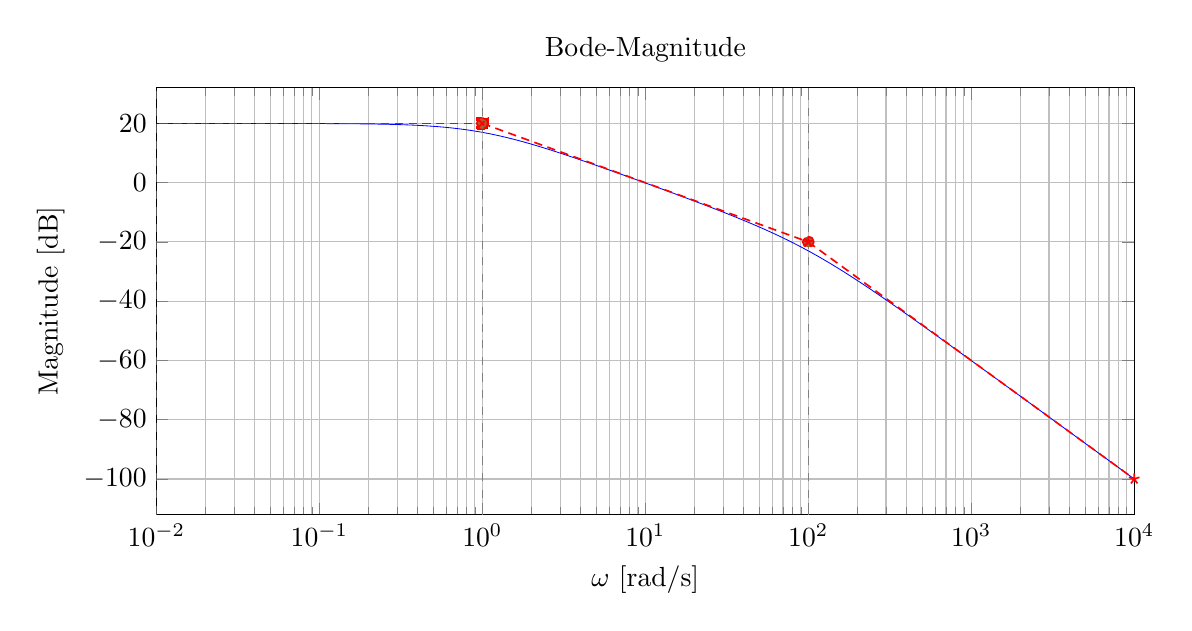
\begin{tikzpicture}
\begin{semilogxaxis}[
  width=14cm,height=7cm,
  xmin=1e-2,xmax=1e4,
  ytick distance=20,
  xlabel={$\omega$ [rad/s]},
  ylabel={Magnitude [dB]},
  grid=both,
  title={Bode-Magnitude}
]
\addplot[
  domain=1e-3:1e4,
  samples=800,
  mark=none,
  line width=0.3pt,
  blue
] {60 - 20*ln(sqrt(1 + x^2))/ln(10) - 20*ln(sqrt(10000 + x^2))/ln(10)};
\addplot+[domain=1e-3:1,samples=2,dashed,dash pattern=on 3pt off 2pt,line width=0.6pt,red] {20};
\addplot+[domain=1:1e2,samples=2,dashed,dash pattern=on 3pt off 2pt,line width=0.6pt,red] {20 - 20*ln(x)/ln(10)};
\addplot+[domain=1e2:1e4,samples=2,dashed,dash pattern=on 3pt off 2pt,line width=0.6pt,red] {-20 - 40*ln(x/100)/ln(10)};
\draw[gray,dashed] (rel axis cs:0,0) -- (rel axis cs:0,1);
\draw[gray,dashed] (axis cs:1,\pgfkeysvalueof{/pgfplots/ymin}) -- (axis cs:1,\pgfkeysvalueof{/pgfplots/ymax});
\draw[gray,dashed] (axis cs:100,\pgfkeysvalueof{/pgfplots/ymin}) -- (axis cs:100,\pgfkeysvalueof{/pgfplots/ymax});
\node[gray,anchor=south east] at (axis cs:1,\pgfkeysvalueof{/pgfplots/ymax}) {\scriptsize Pol $\omega_p=1$};
\node[gray,anchor=south east] at (axis cs:100,\pgfkeysvalueof{/pgfplots/ymax}) {\scriptsize Pol $\omega_p=100$};
\end{semilogxaxis}
\end{tikzpicture}
\vspace{6mm}
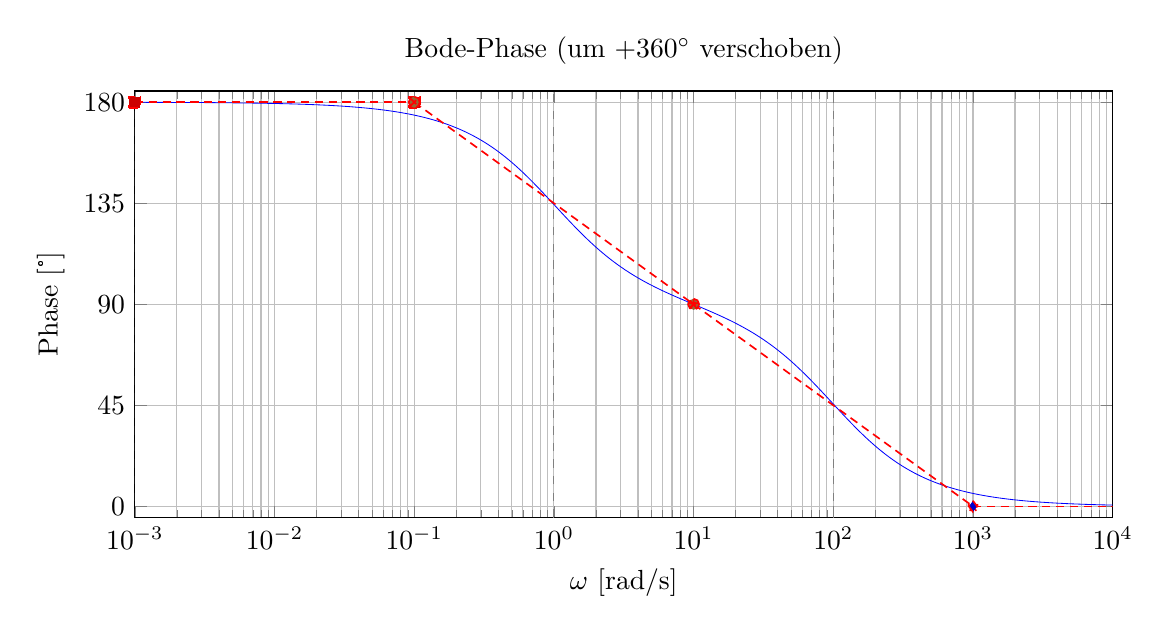
\begin{tikzpicture}
\begin{semilogxaxis}[
  width=14cm,height=7cm,
  xmin=1e-3,xmax=1e4,
  ymin=-5,ymax=185,
  ytick distance=45,
  xlabel={$\omega$ [rad/s]},
  ylabel={Phase [°]},
  grid=both,
  title={Bode-Phase (um $+360^\circ$ verschoben)}
]
\addplot[
  domain=1e-3:1e5,
  samples=800,
  mark=none,
  line width=0.3pt,
  blue
] {180 - atan(x) - atan(x/100)};
\addplot+[domain=1e-3:1e-1,samples=2,dashed,dash pattern=on 3pt off 2pt,line width=0.6pt,red] {180};
\addplot+[domain=1e-1:1e1,samples=2,dashed,dash pattern=on 3pt off 2pt,line width=0.6pt,red] {135 - 45*ln(x)/ln(10)};

\addplot+[domain=1e1:1e3,samples=2,dashed,dash pattern=on 3pt off 2pt,line width=0.6pt,red]{45 - 45*ln(x/100)/ln(10)};
\addplot+[domain=1e3:1e5,samples=2,dashed,dash pattern=on 3pt off 2pt,line width=0.6pt,red]{0};
\draw[gray,dashed] (rel axis cs:0,0) -- (rel axis cs:0,1);
\draw[gray,dashed] (axis cs:1,\pgfkeysvalueof{/pgfplots/ymin}) -- (axis cs:1,\pgfkeysvalueof{/pgfplots/ymax});
\draw[gray,dashed] (axis cs:100,\pgfkeysvalueof{/pgfplots/ymin}) -- (axis cs:100,\pgfkeysvalueof{/pgfplots/ymax});
\node[gray,anchor=south east] at (axis cs:1,\pgfkeysvalueof{/pgfplots/ymax}) {\scriptsize Pol $\omega_p=1$};
\node[gray,anchor=south east] at (axis cs:100,\pgfkeysvalueof{/pgfplots/ymax}) {\scriptsize Pol $\omega_p=100$};
\end{semilogxaxis}
\end{tikzpicture}
\end{center}
\newpage

\subsection{Erklärung}
\begin{description}[leftmargin=1.2em,labelsep=.6em,font=\bfseries]

\item[1. Normalform herstellen.]
\[
H(s)=\frac{-1000}{(s+1)(s+100)}
= \frac{K_0}{(1+sT_{p1})(1+sT_{p2})}
\]
mit
\[
K_0=-10,\quad r=0,\quad T_{p1}=1,\quad T_{p2}=\tfrac{1}{100}.
\]
\[
\underline{F}_1(s)=\frac{1}{1+sT_{p1}}=\frac{1}{1+s},\qquad
\underline{F}_2(s)=\frac{1}{1+sT_{p2}}=\frac{1}{1+\tfrac{s}{100}}.
\]
Konstantes Vorzeichen \(K_0<0\): Phasenoffset \(\pm180^\circ\) (hier Darstellung um \(+360^\circ\) verschoben).

\item[2. Eckfrequenzen bestimmen und sortieren.]Die $\omega$-Eckfrequenzen lassen sich aus den $T_n$'s bestimmen und müssen anschließend sortiert werden:
\[
\omega_{p1}=\frac{1}{T_{p1}}=1\,\mathrm{rad/s},\qquad \omega_{p2}=\frac{1}{T_{p2}}=100\,\mathrm{rad/s},\qquad \omega_{p1}<\omega_{p2}.
\]

\item[3. Startpunkt des Amplitudengangs festlegen (Geradennäherung).]
\[
\omega_{\min}=\omega_{p1}=1,\quad
F_{\mathrm{dB}}(\omega_{\min})=20\log_{10}\!\big(|K_0\underline{F}_{ges}^*(0)|\,\omega_{\min}^{\,r}\big)=20\log_{10}10=20\,\mathrm{dB}.
\]
Unser Ankerpunkt ist: \(20\,\mathrm{dB}\) bei \(\omega=1\).

\item[4. Verlauf links vom Startpunkt zeichnen.]
Für \(\omega<\omega_z\) bleibt die Amplituden-Asymptote bei \(20\,\mathrm{dB}\) konstant (Anfangssteigung \(r\cdot 20 \,\mathrm{dB}=0\)). Zeichne eine waagrechte Gerade links von der kleinsten Eckfrequenz.

\item[5. Steigungswechsel an den Eckfrequenzen eintragen.]
Ab \(\omega=1\): \(-20\,\mathrm{dB/dec}\) (einfacher Pol).
Ab \(\omega=100\): zusätzl. \(-20\,\mathrm{dB/dec}\) \(\Rightarrow\) insgesamt \(-40\,\mathrm{dB/dec}\).
Geradennäherungen:
\[
|H(j\omega)|_{\mathrm{dB}}\approx
\begin{cases}
20,& \omega\le 1,\\
20-20\log_{10}\omega,& 1<\omega\le 100,\\
-20-40\log_{10}(\omega/100),& \omega\ge 100.
\end{cases}
\]

\item[6. Eckabrundungen korrekt berücksichtigen.]
Bei jedem einfachen Pol: \(-3\,\mathrm{dB}\) am Knick.
\[
|H(j1)|_{\mathrm{dB}}=20-10\log_{10}2\approx 17\,\mathrm{dB},\qquad
|H(j100)|_{\mathrm{dB}}=-20-10\log_{10}2\approx -23\,\mathrm{dB}.
\]

\item[7. Phasenstartwert festlegen.]
Wegen \(K_0<0\): Startphase \(-180^\circ + r\cdot90^\circ=-180^\circ\). Darstellung um \(+360^\circ\) verschoben \(\Rightarrow\) \(+180^\circ\) für \(\omega\ll 0.1\).

\item[8. Phasenänderung durch die Polglieder eintragen.]
Jeder einfache Pol: \(-90^\circ\) über je eine Dekade.
Näherung (verschobene Darstellung):
\[
\varphi(\omega)\approx
\begin{cases}
180^\circ,& \omega\le 0.1,\\
135^\circ-45^\circ\log_{10}\omega,& 0.1<\omega<10,\\
45^\circ-45^\circ\log_{10}(\omega/100),& 10<\omega<1000,\\
0^\circ,& \omega\ge 1000.
\end{cases}
\]

\item[9. Grenzwerte und Konsistenz prüfen.]
DC: \(|H(0)|=10\Rightarrow 20\,\mathrm{dB}\); Phase \(-180^\circ\) (hier als \(+180^\circ\) gezeigt).
HF: \(|H(j\omega)|\sim 10/\omega^2\Rightarrow -40\log_{10}(\omega/100)-20\,\mathrm{dB}\). 
Pol-/Nullzählung bestätigt die Endphase: \(m=0\), \(n=2\Rightarrow (m-n)\cdot 90^\circ=-180^\circ\); plus negatives \(K_0\) \(\Rightarrow\) zusätzlich \(-180^\circ\); gesamte \(-360^\circ\equiv 0^\circ\) (mod \(360^\circ\)).

\end{description}

\subsubsection*{Stückweise Näherungen (für die Skizze)}
\[
|H(j\omega)|_{\mathrm{dB}}\approx
\begin{cases}
20,& \omega\ll 1,\\[2pt]
20-10\log_{10}2,& \omega=1,\\[2pt]
20-20\log_{10}\omega,& 1\ll\omega\ll 100,\\[2pt]
-20-10\log_{10}2,& \omega=100,\\[2pt]
-20-40\log_{10}(\omega/100),& \omega\gg 100,
\end{cases}
\]\[
\varphi(\omega)\ (\text{um }+360^\circ)\approx
\begin{cases}
180^\circ,& \omega\le 0.1,\\[2pt]
135^\circ-45^\circ\log_{10}\omega,& 0.1<\omega<10,\\[2pt]
45^\circ-45^\circ\log_{10}(\omega/100),& 10<\omega<1000,\\[2pt]
0^\circ,& \omega\ge 1000.
\end{cases}
\]

\newpage
\section{}
\[
H(s)=\frac{100\,s}{s+1}\,.
\]
\subsection{Bode-Diagramm}
\begin{center}
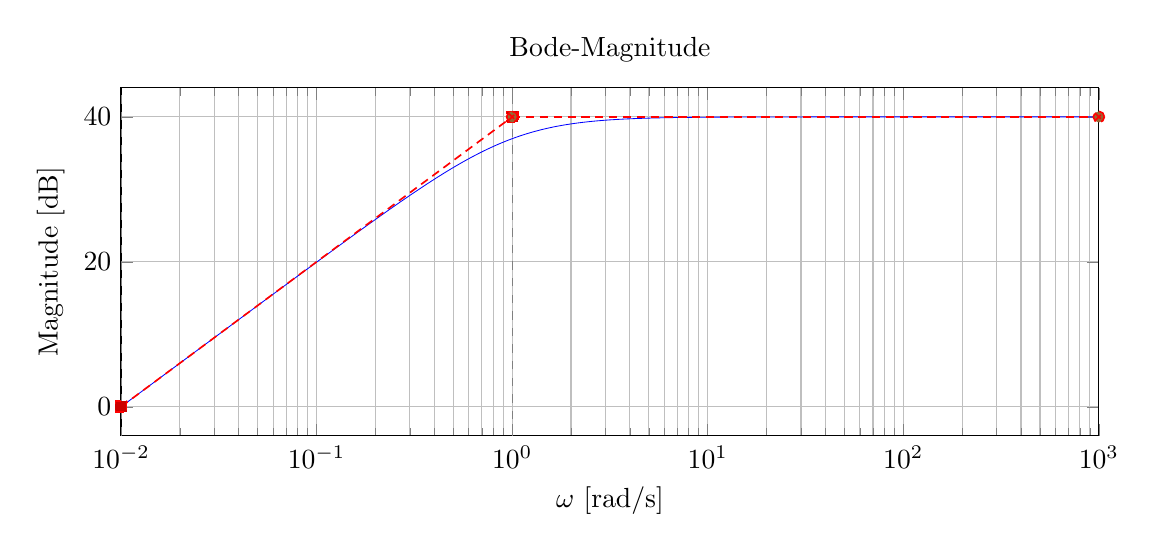
\begin{tikzpicture}
\begin{semilogxaxis}[
  width=14cm,height=6cm,
  xmin=1e-2,xmax=1e3,
  xlabel={$\omega$ [rad/s]},
  ylabel={Magnitude [dB]},
  grid=both,
  title={Bode-Magnitude}
]
\addplot[
  domain=1e-2:1e3,
  samples=600,
  mark=none,
  line width=0.3pt,
  blue
] {40 + 20*ln(x)/ln(10) - 20*ln(sqrt(1 + x^2))/ln(10)};
\addplot+[domain=1e-2:1,samples=2,dashed,dash pattern=on 3pt off 2pt,line width=0.6pt,red] {40 + 20*ln(x)/ln(10)};
\addplot+[domain=1:1e3,samples=2,dashed,dash pattern=on 3pt off 2pt,line width=0.6pt,red] {40};
\draw[gray,dashed] (rel axis cs:0,0) -- (rel axis cs:0,1);
\draw[gray,dashed] (axis cs:1,\pgfkeysvalueof{/pgfplots/ymin}) -- (axis cs:1,\pgfkeysvalueof{/pgfplots/ymax});
\node[gray,anchor=south east] at (axis cs:1,\pgfkeysvalueof{/pgfplots/ymax}) {\scriptsize Pol $\omega_p=1$};
\end{semilogxaxis}
\end{tikzpicture}
\vspace{6mm}
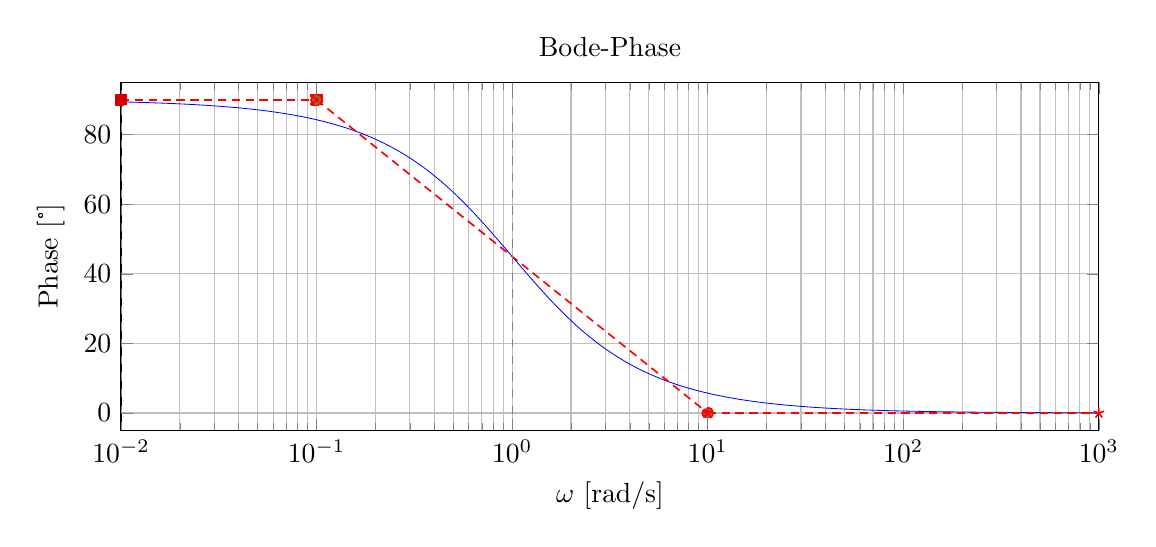
\begin{tikzpicture}
\begin{semilogxaxis}[
  width=14cm,height=6cm,
  xmin=1e-2,xmax=1e3,
  ymin=-5,ymax=95,
  xlabel={$\omega$ [rad/s]},
  ylabel={Phase [°]},
  grid=both,
  title={Bode-Phase}
]
\addplot[
  domain=1e-2:1e3,
  samples=600,
  mark=none,
  line width=0.3pt,
  blue
] {90 - atan(x)};
\addplot+[domain=1e-2:1e-1,samples=2,dashed,dash pattern=on 3pt off 2pt,line width=0.6pt,red] {90};
\addplot+[domain=1e-1:1e1,samples=2,dashed,dash pattern=on 3pt off 2pt,line width=0.6pt,red] {45 - 45*ln(x)/ln(10)};
\addplot+[domain=1e1:1e3,samples=2,dashed,dash pattern=on 3pt off 2pt,line width=0.6pt,red] {0};
\draw[gray,dashed] (rel axis cs:0,0) -- (rel axis cs:0,1);
\draw[gray,dashed] (axis cs:1,\pgfkeysvalueof{/pgfplots/ymin}) -- (axis cs:1,\pgfkeysvalueof{/pgfplots/ymax});
\node[gray,anchor=south east] at (axis cs:1,\pgfkeysvalueof{/pgfplots/ymax}) {\scriptsize Pol $\omega_p=1$};
\end{semilogxaxis}
\end{tikzpicture}
\end{center}
\newpage
\subsection{Erklärung}
\vspace{5mm}
\begin{description}[leftmargin=1.2em,labelsep=.6em,font=\bfseries]
\item[Schritt 1] DC-Faktor $100$: Betrag global um $+40\,\mathrm{dB}$ verschoben; die konstante (reell-positive) Verstärkung ändert die Steigung nicht und fügt keine zusätzliche Phase hinzu. Referenzniveau der Geradennäherung damit bei $40\,\mathrm{dB}$.
\item[Schritt 2] Nullstelle im Ursprung: Startsteigung $+20\,\mathrm{dB/dec}$ für $\omega\ll1$, da $|H(\j\omega)|\sim100\,\omega$; Startphase $\approx+90^\circ$ (ideale Integrationsumkehr). In der Magnituden-Näherung ergibt sich links der Ecke die Gerade $40+20\log_{10}\omega$.
\item[Schritt 3] Pol bei $\omega_p=1\,\mathrm{rad/s}$: ab $\omega=1$ Steigungswechsel um $-20\,\mathrm{dB/dec}$; resultierend flacht die Magnitude auf $0\,\mathrm{dB/dec}$ ab und nähert sich für $\omega\gg1$ dem konstanten Niveau $\approx40\,\mathrm{dB}$. Exakter Eckpunkt: $40-10\log_{10}2\approx36.99\,\mathrm{dB}$. Die Phase fällt über die Übergangsdekade $\omega_l=0.1$ bis $\omega_h=10\,\mathrm{rad/s}$ von $\approx+90^\circ$ gegen $0^\circ$ (Geradennäherung: $45^\circ-45^\circ\log_{10}\omega$ in $[0.1,10]$).
\end{description}

\vspace{0.5cm}
\medskip
\noindent\textbf{Stückweise Näherung}
\[
|H(\j\omega)|_{\mathrm{dB}}\approx
\begin{cases}
40+20\log_{10}\omega,& \omega\ll1,\\[4pt]
40-10\log_{10}2,& \omega=1,\\[4pt]
40,& \omega\gg1,
\end{cases}
\qquad
\]
\newpage
\section{}
\[
H(s)=\frac{10\sqrt{2}\,s^{2}}{s-1}\,.
\]
\subsection{Bode-Diagramm}
\begin{center}
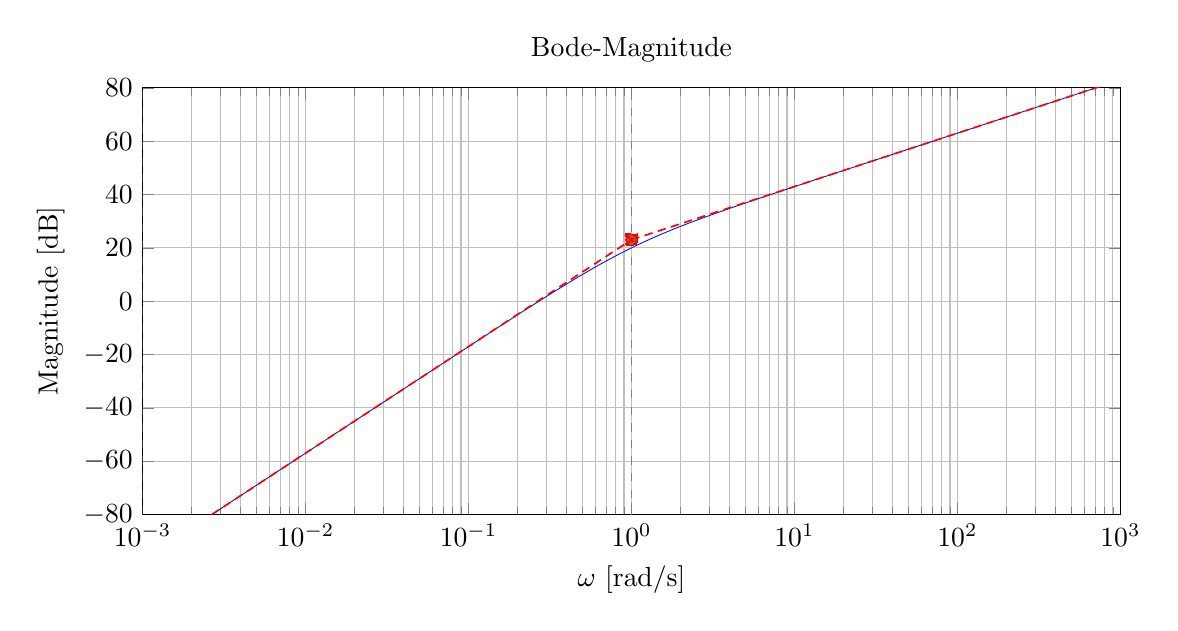
\begin{tikzpicture}
\begin{semilogxaxis}[
  width=14cm,height=7cm,
  xmin=1e-3,xmax=1e3,
  ymin=-80,ymax=80,
  xlabel={$\omega$ [rad/s]},
  ylabel={Magnitude [dB]},
  ytick distance=20,
  grid=both,
  title={Bode-Magnitude}
]
\addplot[
  domain=1e-3:1e3,
  samples=600,
  mark=none,
  line width=0.3pt,
  blue
] {20 + 10*ln(2)/ln(10) + 40*ln(x)/ln(10) - 10*ln(1 + x^2)/ln(10)};
\addplot+[domain=1e-3:1,samples=2,dashed,dash pattern=on 3pt off 2pt,line width=0.6pt,red] {20 + 10*ln(2)/ln(10) + 40*ln(x)/ln(10)};
\addplot+[domain=1:1e3,samples=2,dashed,dash pattern=on 3pt off 2pt,line width=0.6pt,red] {20 + 10*ln(2)/ln(10) + 20*ln(x)/ln(10)};
\draw[gray,dashed] (rel axis cs:0,0) -- (rel axis cs:0,1);
\draw[gray,dashed] (axis cs:1,\pgfkeysvalueof{/pgfplots/ymin}) -- (axis cs:1,\pgfkeysvalueof{/pgfplots/ymax});
\node[gray,anchor=south east] at (axis cs:1,\pgfkeysvalueof{/pgfplots/ymax}) {\scriptsize Pol $\omega_p=1$ (RHP)};
\end{semilogxaxis}
\end{tikzpicture}
\vspace{6mm}
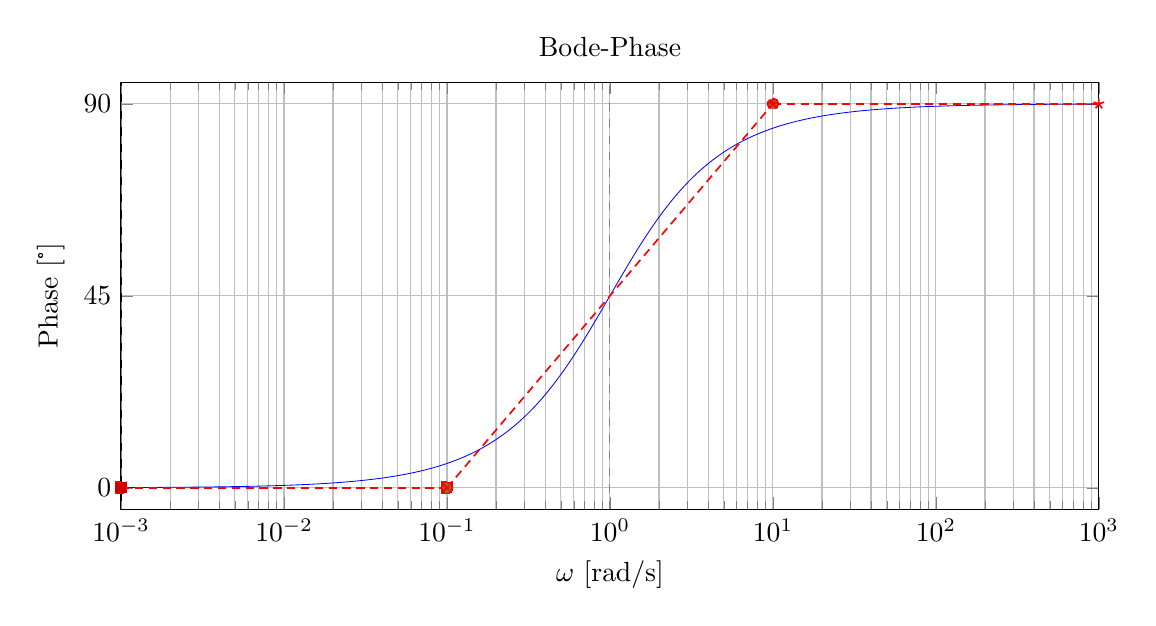
\begin{tikzpicture}
\begin{semilogxaxis}[
  width=14cm,height=7cm,
  xmin=1e-3,xmax=1e3,
  ymin=-5,ymax=95,
  ytick distance=45,
  xlabel={$\omega$ [rad/s]},
  ylabel={Phase [°]},
  grid=both,
  title={Bode-Phase}
]
\addplot[
  domain=1e-3:1e3,
  samples=600,
  mark=none,
  line width=0.3pt,
  blue
] {atan(x)};
\addplot+[domain=1e-3:1e-1,samples=2,dashed,dash pattern=on 3pt off 2pt,line width=0.6pt,red] {0};
\addplot+[domain=1e-1:1e1,samples=2,dashed,dash pattern=on 3pt off 2pt,line width=0.6pt,red] {45 + 45*ln(x)/ln(10)};
\addplot+[domain=1e1:1e3,samples=2,dashed,dash pattern=on 3pt off 2pt,line width=0.6pt,red] {90};
\draw[gray,dashed] (rel axis cs:0,0) -- (rel axis cs:0,1);
\draw[gray,dashed] (axis cs:1,\pgfkeysvalueof{/pgfplots/ymin}) -- (axis cs:1,\pgfkeysvalueof{/pgfplots/ymax});
\node[gray,anchor=south east] at (axis cs:1,\pgfkeysvalueof{/pgfplots/ymax}) {\scriptsize Pol $\omega_p=1$ (RHP)};
\end{semilogxaxis}
\end{tikzpicture}
\end{center}
\newpage
\subsection{Erklärung}
\vspace{5mm}
\begin{description}[leftmargin=1.2em,labelsep=.6em,font=\bfseries]
\item[Schritt 1] Doppelnullstelle im Ursprung: Startsteigung $+40\,\mathrm{dB/dec}$; Startphase $0^\circ$.
\item[Schritt 2] RHP-Pol bei $\omega_p=1\,\mathrm{rad/s}$: ab $\omega=1$ Steigungsänderung $-20\,\mathrm{dB/dec}$; Netto $+20\,\mathrm{dB/dec}$ für $\omega\gg1$. Phasen-Geradennäherung in $45^\circ$-Schritten: $0^\circ$ für $\omega\le0.1$, $45^\circ+45\log_{10}\omega$ in $[0.1,10]$, $90^\circ$ für $\omega\ge10$.
\item[Schritt 3] Grenzwerte: $|H|_{\mathrm{dB}}\approx 20+10\log_{10}2+40\log_{10}\omega$ für $\omega\ll1$, und $20+10\log_{10}2+20\log_{10}\omega$ für $\omega\gg1$; $\angle H\to90^\circ$ für große $\omega$.
\end{description}

\vspace{0.5cm}
\medskip
\noindent\textbf{Stückweise Näherung}
\[
|H(\j\omega)|_{\mathrm{dB}}\approx
\begin{cases}
20+10\log_{10}2+40\log_{10}\omega,& \omega\ll1,\\[4pt]
20,& \omega=1,\\[4pt]
20+10\log_{10}2+20\log_{10}\omega,& \omega\gg1,
\end{cases}
\qquad
\]
\newpage
\section{}
\[
H(s)=\frac{s+1}{(s+10)^2}\,.
\]
\subsection{Bode-Diagramm}
\begin{center}
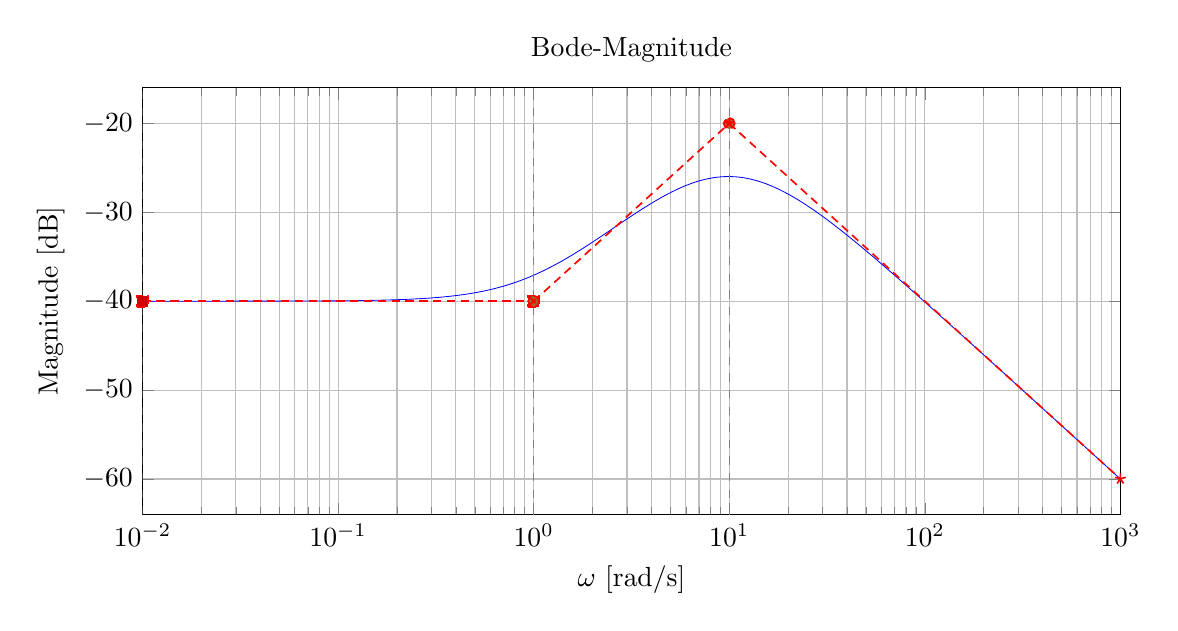
\begin{tikzpicture}
\begin{semilogxaxis}[
  width=14cm,height=7cm,
  xmin=1e-2,xmax=1e3,
  xlabel={$\omega$ [rad/s]},
  ylabel={Magnitude [dB]},
  grid=both,
  title={Bode-Magnitude}
]
\addplot[
  domain=1e-2:1e3,
  samples=600,
  mark=none,
  line width=0.3pt,
  blue
] {20*ln(sqrt(1 + x^2))/ln(10) - 40*ln(sqrt(100 + x^2))/ln(10)};
\addplot+[domain=1e-2:1,samples=2,dashed,dash pattern=on 3pt off 2pt,line width=0.6pt,red] {-40};
\addplot+[domain=1:1e1,samples=2,dashed,dash pattern=on 3pt off 2pt,line width=0.6pt,red] {-40 + 20*ln(x)/ln(10)};
\addplot+[domain=1e1:1e3,samples=2,dashed,dash pattern=on 3pt off 2pt,line width=0.6pt,red] {-20 - 20*ln(x/10)/ln(10)};
\draw[gray,dashed] (rel axis cs:0,0) -- (rel axis cs:0,1);
\draw[gray,dashed] (axis cs:1,\pgfkeysvalueof{/pgfplots/ymin}) -- (axis cs:1,\pgfkeysvalueof{/pgfplots/ymax});
\draw[gray,dashed] (axis cs:10,\pgfkeysvalueof{/pgfplots/ymin}) -- (axis cs:10,\pgfkeysvalueof{/pgfplots/ymax});
\node[gray,anchor=south east] at (axis cs:1,\pgfkeysvalueof{/pgfplots/ymax}) {\scriptsize Nullstelle $\omega_z=1$};
\node[gray,anchor=south east] at (axis cs:10,\pgfkeysvalueof{/pgfplots/ymax}) {\scriptsize Pol $\omega_p=10$ (doppelt)};
\end{semilogxaxis}
\end{tikzpicture}
\vspace{6mm}
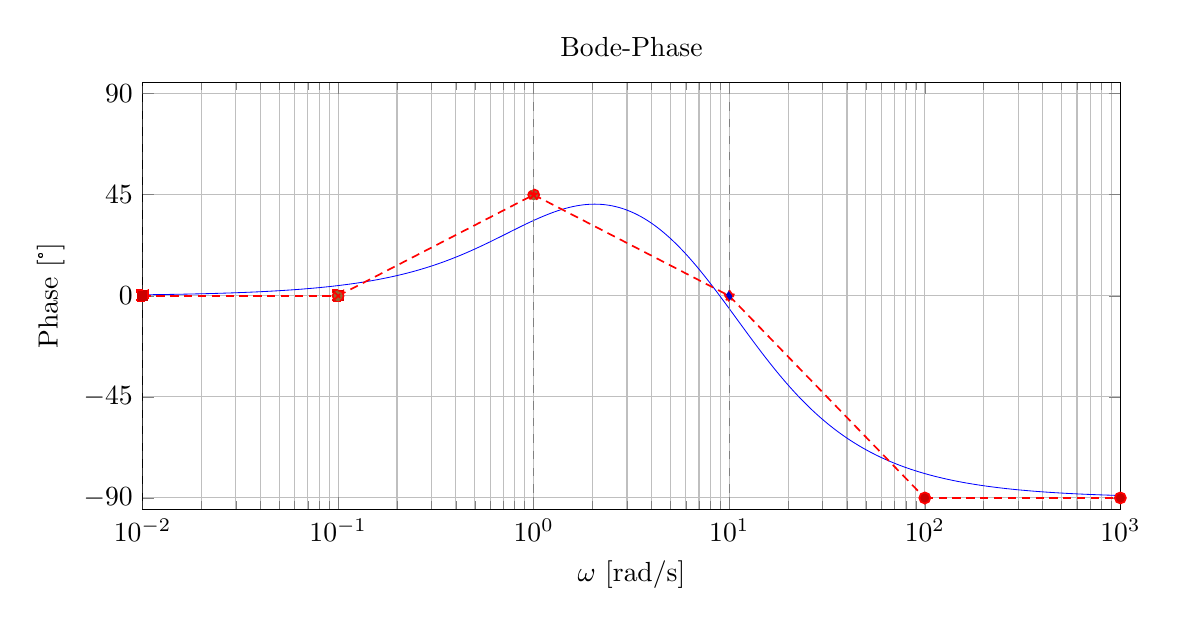
\begin{tikzpicture}
\begin{semilogxaxis}[
  width=14cm,height=7cm,
  xmin=1e-2,xmax=1e3,
  ytick distance=45,
  ymin=-95,ymax=95,
  xlabel={$\omega$ [rad/s]},
  ylabel={Phase [°]},
  grid=both,
  title={Bode-Phase}
]
\addplot[
  domain=1e-2:1e3,
  samples=600,
  mark=none,
  line width=0.3pt,
  blue
] {atan(x) - 2*atan(x/10)};
\addplot+[domain=1e-2:1e-1,samples=2,dashed,dash pattern=on 3pt off 2pt,line width=0.6pt,red] {0};
\addplot+[domain=1e-1:1e0,samples=2,dashed,dash pattern=on 3pt off 2pt,line width=0.6pt,red] {45 + 45*ln(x)/ln(10)};
\addplot+[domain=1e0:1e1,samples=2,dashed,dash pattern=on 3pt off 2pt,line width=0.6pt,red] {45 - 45*ln(x)/ln(10)};
\addplot+[domain=1e1:1e2,samples=2,dashed,dash pattern=on 3pt off 2pt,line width=0.6pt,red] {-90*ln(x/10)/ln(10)};
\addplot+[domain=1e2:1e3,samples=2,dashed,dash pattern=on 3pt off 2pt,line width=0.6pt,red] {-90};
\draw[gray,dashed] (rel axis cs:0,0) -- (rel axis cs:0,1);
\draw[gray,dashed] (axis cs:1,\pgfkeysvalueof{/pgfplots/ymin}) -- (axis cs:1,\pgfkeysvalueof{/pgfplots/ymax});
\draw[gray,dashed] (axis cs:10,\pgfkeysvalueof{/pgfplots/ymin}) -- (axis cs:10,\pgfkeysvalueof{/pgfplots/ymax});
\node[gray,anchor=south east] at (axis cs:1,\pgfkeysvalueof{/pgfplots/ymax}) {\scriptsize Nullstelle $\omega_z=1$};
\node[gray,anchor=south east] at (axis cs:10,\pgfkeysvalueof{/pgfplots/ymax}) {\scriptsize Pol $\omega_p=10$ (doppelt)};
\end{semilogxaxis}
\end{tikzpicture}
\end{center}
\newpage
\subsection{Erklärung}
\begin{description}[leftmargin=1.2em,labelsep=.6em,font=\bfseries]

\item[1. Normalform herstellen.]
Bringe die Übertragungsfunktion exakt in die im Skript definierte Standardform.
\[
H(s)=\frac{s+1}{(s+10)^2}
= K_0\cdot(1+sT_z)\cdot\frac{1}{(1+sT_p)^2}
\]
mit
\[
K_0=\frac{1}{100},\quad r=0,\quad T_z=1,\quad T_p=\tfrac{1}{10}.
\]
\[
\underline{F}_1(s)=1+sT_z\quad\text{(LHP-Nullstelle)},\qquad
\underline{F}_2(s)=\frac{1}{(1+sT_p)^2}\quad\text{(Doppelpol)}.
\]

\item[2. Eckfrequenzen bestimmen und sortieren.] Die $\omega$-Eckfrequenzen lassen sich aus den $T_n$'s bestimmen und müssen anschließend sortiert werden:
\[
\omega_z=\frac{1}{T_z}=1\,\mathrm{rad/s},\qquad \omega_p=\frac{1}{T_p}=10\,\mathrm{rad/s},\qquad \omega_z<\omega_p.
\]

\item[3. Startpunkt des Amplitudengangs festlegen (Geradennäherung).]
Setze \(\omega_{\min}=\omega_z=1\).
\[
F_{\mathrm{dB}}(\omega_{\min})=20\log_{10}\!\Big(|K_0F^*_{ges}(0)|\,\omega_{\min}^{\,r}\Big)
=20\log_{10}\!\Big(\frac{1}{100}\cdot 1\cdot 1^{0}\Big)=-40\,\mathrm{dB}.
\]
Ankerpunkt: \(-40\,\mathrm{dB}\) bei \(\omega=1\).

\item[4. Verlauf links vom Startpunkt zeichnen.]
Für \(\omega<1\): Anfangssteigung \(r\cdot 20=0\,\mathrm{dB/dec}\) \(\Rightarrow\) horizontale Asymptote bei \(-40\,\mathrm{dB}\).

\item[5. Steigungswechsel an den Eckfrequenzen eintragen.]
Nullstelle bei \(\omega_z=1\): \(+20\,\mathrm{dB/dec}\) ab \(\omega=1\).
Doppelpol bei \(\omega_p=10\): zusätzlich \(-40\,\mathrm{dB/dec}\) ab \(\omega=10\), also insgesamt \(-20\,\mathrm{dB/dec}\).
Netto:
\[
\begin{cases}
-40\,\mathrm{dB}\ \text{(flach)},& \omega<1,\\
-40+20\log_{10}\omega,& 1\le \omega<10\ \text{(Steigung }+20\,\mathrm{dB/dec}),\\
-20-20\log_{10}(\omega/10),& \omega\ge 10\ \text{(Steigung }-20\,\mathrm{dB/dec}).
\end{cases}
\]

\item[6. Eckabrundung korrekt berücksichtigen.]
LHP-Nullstelle: bei \(\omega=1\) liegt der exakte Betrag um \(+3\,\mathrm{dB}\) über der Gerade:
\[
|H(j1)|_{\mathrm{dB}}=10\log_{10}2-20\log_{10}101\approx -37\,\mathrm{dB}.
\]
Doppelpol: bei \(\omega=10\) insgesamt \(-6\,\mathrm{dB}\) unter der Asymptote:
\[
|H(j10)|_{\mathrm{dB}}=10\log_{10}101-20\log_{10}200\approx -26\,\mathrm{dB}.
\]

\item[7. Phasenstartwert festlegen.]
Da \(K_0\underline{F}_{ges}^*(0)>0\), \(r=0\) \(\Rightarrow\) \(\varphi(0)=r\cdot90^\circ=0^\circ\).

\item[8. Phasenänderung durch Nullstelle und Doppelpol eintragen.]
Nullstelle bewirkt eine Phasenänderung um \(+90^\circ\) über \([0.1,10]\). Jeder Pol \(-90^\circ\) über \([1,100]\) (zwei Pole \(\Rightarrow -180^\circ\) total). Die Effekte überlappen sich in $[1,10]$; dort addieren sich die Steigungen.
Näherung:
\[
\varphi(\omega)\approx
\begin{cases}
0^\circ,& \omega\le 0.1,\\
45^\circ+45^\circ\log_{10}\omega,& 0.1<\omega<1,\\
45^\circ-45^\circ\log_{10}\omega,& 1<\omega<10,\\
-90^\circ\log_{10}(\omega/10),& 10<\omega<100,\\
-90^\circ,& \omega\ge 100.
\end{cases}
\]

\item[9. Grenzwerte und Konsistenz prüfen.]
DC: \(|H(0)|=\tfrac{1}{100}\Rightarrow -40\,\mathrm{dB}\), \(\varphi(0)=0^\circ\).
HF: \(|H(j\omega)|\sim \omega/\omega^2=1/\omega\Rightarrow -20\log_{10}(\omega/10)-20\,\mathrm{dB}\).
Pol-/Nullzählung: \(m=1\), \(n=2\Rightarrow (m-n)\cdot 90^\circ=-90^\circ\) \(\Rightarrow \varphi(\infty)=-90^\circ\).

\end{description}

\subsubsection*{Stückweise Näherungen (für die Skizze)}
\[
|H(j\omega)|_{\mathrm{dB}}\approx
\begin{cases}
-40,& \omega\ll 1,\\[2pt]
-40+20\log_{10}\omega,& 1\ll\omega\ll 10,\\[2pt]
-20-20\log_{10}(\omega/10),& \omega\gg 10,
\end{cases}
\]\[
\varphi(\omega)\approx
\begin{cases}
0^\circ,& \omega\le 0.1,\\[2pt]
45^\circ+45^\circ\log_{10}\omega,& 0.1<\omega<1,\\[2pt]
45^\circ-45^\circ\log_{10}\omega,& 1<\omega<10,\\[2pt]
-90^\circ\log_{10}(\omega/10),& 10<\omega<100,\\[2pt]
-90^\circ,& \omega\ge 100.
\end{cases}
\]

\newpage
\section{}
\[
H(s)=\frac{s+1}{s^2+2s+1}=\frac{1}{s+1}\,.
\]
\subsection{Bode-Diagramm}
\begin{center}
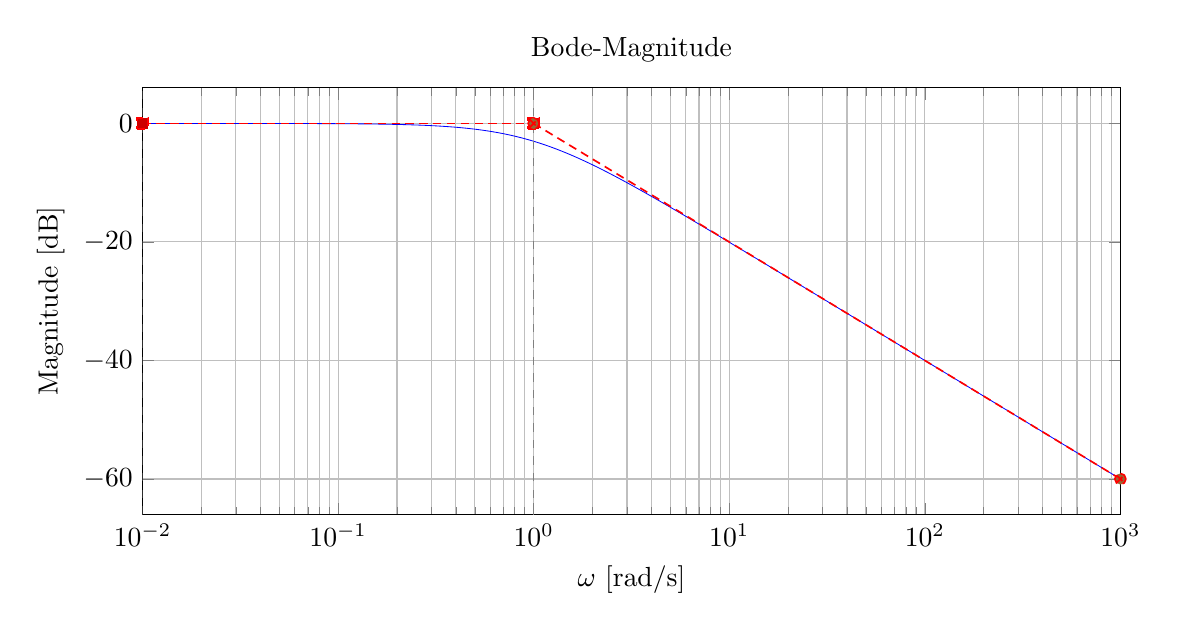
\begin{tikzpicture}
\begin{semilogxaxis}[
  width=14cm,height=7cm,
  xmin=1e-2,xmax=1e3,
  xlabel={$\omega$ [rad/s]},
  ylabel={Magnitude [dB]},
  grid=both,
  title={Bode-Magnitude}
]
\addplot[
  domain=1e-2:1e3,
  samples=600,
  mark=none,
  line width=0.3pt,
  blue
] {-20*ln(sqrt(1 + x^2))/ln(10)};
\addplot+[domain=1e-2:1,samples=2,dashed,dash pattern=on 3pt off 2pt,line width=0.6pt,red] {0};
\addplot+[domain=1:1e3,samples=2,dashed,dash pattern=on 3pt off 2pt,line width=0.6pt,red] {-20*ln(x)/ln(10)};
\draw[gray,dashed] (rel axis cs:0,0) -- (rel axis cs:0,1);
\draw[gray,dashed] (axis cs:1,\pgfkeysvalueof{/pgfplots/ymin}) -- (axis cs:1,\pgfkeysvalueof{/pgfplots/ymax});
\node[gray,anchor=south east] at (axis cs:1,\pgfkeysvalueof{/pgfplots/ymax}) {\scriptsize Pol $\omega_p=1$};
\end{semilogxaxis}
\end{tikzpicture}
\vspace{6mm}
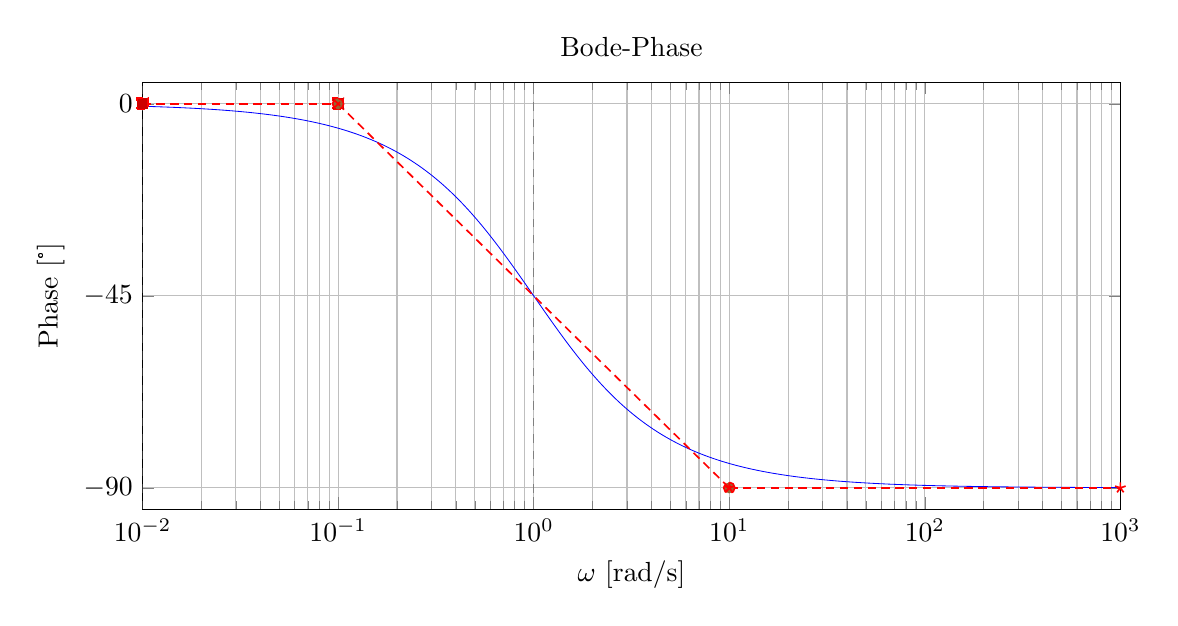
\begin{tikzpicture}
\begin{semilogxaxis}[
  width=14cm,height=7cm,
  xmin=1e-2,xmax=1e3,
  ymin=-95,ymax=5,
  ytick distance=45,
  xlabel={$\omega$ [rad/s]},
  ylabel={Phase [°]},
  grid=both,
  title={Bode-Phase}
]
\addplot[
  domain=1e-2:1e3,
  samples=600,
  mark=none,
  line width=0.3pt,
  blue
] {-atan(x)};
\addplot+[domain=1e-2:1e-1,samples=2,dashed,dash pattern=on 3pt off 2pt,line width=0.6pt,red] {0};
\addplot+[domain=1e-1:1e1,samples=2,dashed,dash pattern=on 3pt off 2pt,line width=0.6pt,red] {-45 - 45*ln(x)/ln(10)};
\addplot+[domain=1e1:1e3,samples=2,dashed,dash pattern=on 3pt off 2pt,line width=0.6pt,red] {-90};
\draw[gray,dashed] (rel axis cs:0,0) -- (rel axis cs:0,1);
\draw[gray,dashed] (axis cs:1,\pgfkeysvalueof{/pgfplots/ymin}) -- (axis cs:1,\pgfkeysvalueof{/pgfplots/ymax});
\node[gray,anchor=south east] at (axis cs:1,\pgfkeysvalueof{/pgfplots/ymax}) {\scriptsize Pol $\omega_p=1$};
\end{semilogxaxis}
\end{tikzpicture}
\end{center}
\newpage
\subsection{Erklärung}
\vspace{5mm}
\begin{description}[leftmargin=1.2em,labelsep=.6em,font=\bfseries]
\item[Schritt 1] Kürzung: $s^2+2s+1=(s+1)^2\Rightarrow H(s)=\dfrac{s+1}{(s+1)^2}=\dfrac{1}{s+1}$. DC-Faktor $1$: für $\omega\ll1$ gilt $|H(\j\omega)|\approx1$; Betrag $0\,\mathrm{dB}$ ohne Anfangssteigung, Phase $\approx0^\circ$.
\item[Schritt 2] Einfacher Pol bei $\omega_p=1\,\mathrm{rad/s}$: ab $\omega=1$ wechselt die Magnituden-Steigung um $-20\,\mathrm{dB/dec}$. Am Eckpunkt beträgt die exakte Dämpfung $-10\log_{10}2\approx-3.01\,\mathrm{dB}$ relativ zur Geraden. Phasenübergang über $\omega\in[0.1,10]$ von $0^\circ$ nach $-90^\circ$; Geradennäherung: $-45^\circ-45\log_{10}\omega$.
\item[Schritt 3] Grenzverhalten: für $\omega\gg1$ folgt $|H(\j\omega)|_{\mathrm{dB}}\approx-20\log_{10}\omega$; die Phase nähert sich $-90^\circ$. Für $\omega\ll1$ bleibt $|H|\approx1$ und $\angle H\approx0^\circ$.
\end{description}

\vspace{0.5cm}
\medskip
\noindent\textbf{Stückweise Näherung}
\[
|H(\j\omega)|_{\mathrm{dB}}\approx
\begin{cases}
0,& \omega\ll1,\\[4pt]
-10\log_{10}2,& \omega=1,\\[4pt]
-20\log_{10}\omega,& \omega\gg1,
\end{cases}
\qquad
\]
\newpage
\section{}
\[
H(s)=\frac{100\,(s+1)}{s^2+20s+100}=\frac{100\,(s+1)}{(s+10)^2}\,.
\]
\subsection{Bode-Diagramm}
\begin{center}
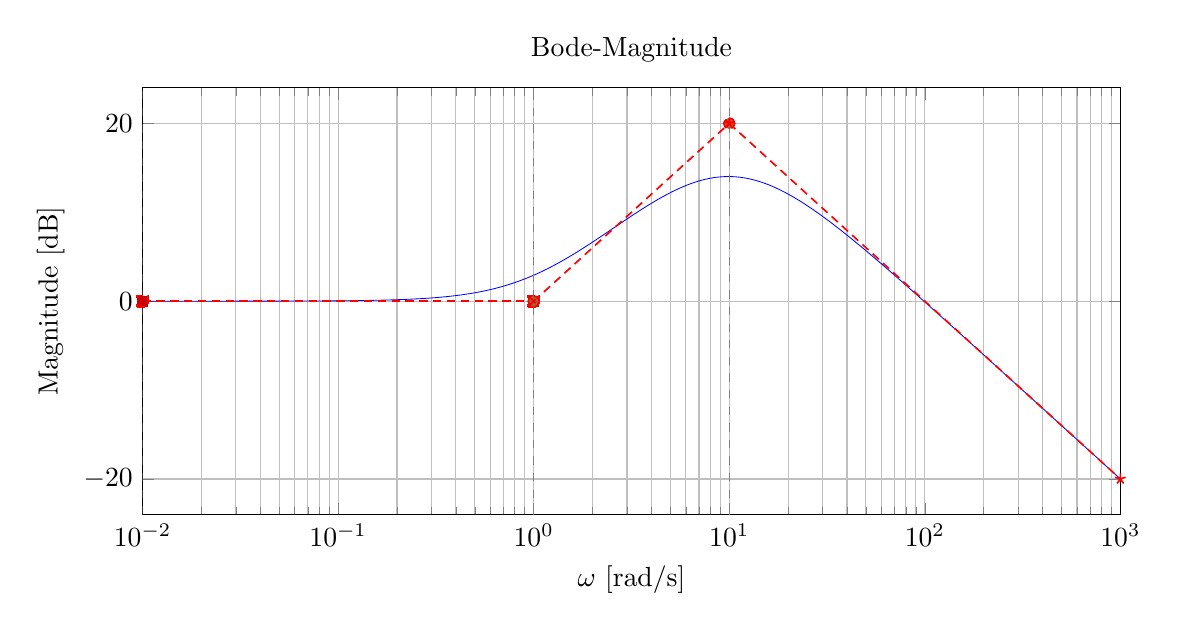
\begin{tikzpicture}
\begin{semilogxaxis}[
  width=14cm,height=7cm,
  xmin=1e-2,xmax=1e3,
  xlabel={$\omega$ [rad/s]},
  ylabel={Magnitude [dB]},
  grid=both,
  ytick distance=20,
  title={Bode-Magnitude}
]
\addplot[
  domain=1e-2:1e3,
  samples=600,
  mark=none,
  line width=0.3pt,
  blue
] {40 + 20*ln(sqrt(1 + x^2))/ln(10) - 40*ln(sqrt(100 + x^2))/ln(10)};
\addplot+[domain=1e-2:1,samples=2,dashed,dash pattern=on 3pt off 2pt,line width=0.6pt,red] {0};
\addplot+[domain=1:1e1,samples=2,dashed,dash pattern=on 3pt off 2pt,line width=0.6pt,red] {20*ln(x)/ln(10)};
\addplot+[domain=1e1:1e3,samples=2,dashed,dash pattern=on 3pt off 2pt,line width=0.6pt,red] {20 - 20*ln(x/10)/ln(10)};
\draw[gray,dashed] (rel axis cs:0,0) -- (rel axis cs:0,1);
\draw[gray,dashed] (axis cs:1,\pgfkeysvalueof{/pgfplots/ymin}) -- (axis cs:1,\pgfkeysvalueof{/pgfplots/ymax});
\draw[gray,dashed] (axis cs:10,\pgfkeysvalueof{/pgfplots/ymin}) -- (axis cs:10,\pgfkeysvalueof{/pgfplots/ymax});
\node[gray,anchor=south east] at (axis cs:1,\pgfkeysvalueof{/pgfplots/ymax}) {\scriptsize Nullstelle $\omega_z=1$};
\node[gray,anchor=south east] at (axis cs:10,\pgfkeysvalueof{/pgfplots/ymax}) {\scriptsize Pol $\omega_p=10$ (doppelt)};
\end{semilogxaxis}
\end{tikzpicture}
\vspace{6mm}
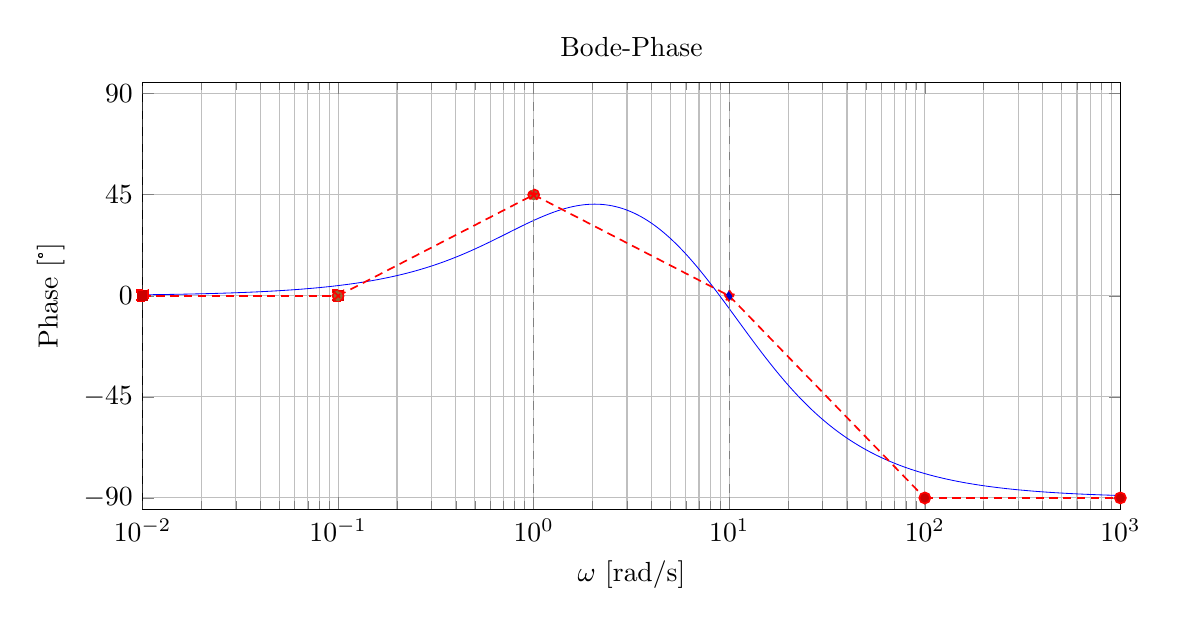
\begin{tikzpicture}
\begin{semilogxaxis}[
  width=14cm,height=7cm,
  xmin=1e-2,xmax=1e3,
  ymin=-95,ymax=95,
  ytick distance=45,
  xlabel={$\omega$ [rad/s]},
  ylabel={Phase [°]},
  grid=both,
  title={Bode-Phase}
]
\addplot[
  domain=1e-2:1e3,
  samples=600,
  mark=none,
  line width=0.3pt,
  blue
] {atan(x) - 2*atan(x/10)};
\addplot+[domain=1e-2:1e-1,samples=2,dashed,dash pattern=on 3pt off 2pt,line width=0.6pt,red] {0};
\addplot+[domain=1e-1:1e0,samples=2,dashed,dash pattern=on 3pt off 2pt,line width=0.6pt,red] {45 + 45*ln(x)/ln(10)};
\addplot+[domain=1e0:1e1,samples=2,dashed,dash pattern=on 3pt off 2pt,line width=0.6pt,red] {45 - 45*ln(x)/ln(10)};
\addplot+[domain=1e1:1e2,samples=2,dashed,dash pattern=on 3pt off 2pt,line width=0.6pt,red] {-90*ln(x/10)/ln(10)};
\addplot+[domain=1e2:1e3,samples=2,dashed,dash pattern=on 3pt off 2pt,line width=0.6pt,red] {-90};
\draw[gray,dashed] (rel axis cs:0,0) -- (rel axis cs:0,1);
\draw[gray,dashed] (axis cs:1,\pgfkeysvalueof{/pgfplots/ymin}) -- (axis cs:1,\pgfkeysvalueof{/pgfplots/ymax});
\draw[gray,dashed] (axis cs:10,\pgfkeysvalueof{/pgfplots/ymin}) -- (axis cs:10,\pgfkeysvalueof{/pgfplots/ymax});
\node[gray,anchor=south east] at (axis cs:1,\pgfkeysvalueof{/pgfplots/ymax}) {\scriptsize Nullstelle $\omega_z=1$};
\node[gray,anchor=south east] at (axis cs:10,\pgfkeysvalueof{/pgfplots/ymax}) {\scriptsize Pol $\omega_p=10$ (doppelt)};
\end{semilogxaxis}
\end{tikzpicture}
\end{center}
\newpage
\subsection{Erklärung}
\begin{description}[leftmargin=1.2em,labelsep=.6em,font=\bfseries]

\item[1. Normalform herstellen.]
\[
H(s)=\frac{100(s+1)}{(s+10)^2}
= K_0\cdot(1+sT_z)\cdot\frac{1}{(1+sT_p)^2}
\]
mit
\[
K_0=1,\quad r=0,\quad T_z=1,\quad T_p=\tfrac{1}{10}.
\]
\[
\underline{F}_1(s)=1+sT_z\quad\text{(LHP-Nullstelle)},\qquad
\underline{F}_2(s)=\frac{1}{(1+sT_p)^2}\quad\text{(Doppelpol)}.
\]

\item[2. Eckfrequenzen bestimmen und sortieren.] Die $\omega$-Eckfrequenzen aus den $T_n$ bestimmen und sortieren:
\[
\omega_z=\frac{1}{T_z}=1\,\mathrm{rad/s},\qquad
\omega_p=\frac{1}{T_p}=10\,\mathrm{rad/s},\qquad
\omega_z<\omega_p.
\]

\item[3. Startpunkt des Amplitudengangs festlegen (Geradennäherung).]
Setze \(\omega_{\min}=\omega_z=1\).
\[
F_{\mathrm{dB}}(\omega_{\min})=20\log_{10}\!\Big(|K_0F^*_{ges}(0)|\,\omega_{\min}^{\,r}\Big)
=20\log_{10}(1)=0\,\mathrm{dB}.
\]
Ankerpunkt: \(0\,\mathrm{dB}\) bei \(\omega=1\).

\item[4. Verlauf links vom Startpunkt zeichnen.]
Für \(\omega<1\) bleibt die Amplituden-Asymptote bei \(0\,\mathrm{dB}\) konstant (Anfangssteigung \(r\cdot 20\,\mathrm{dB/dec}=0\)). Zeichne links von der kleinsten Eckfrequenz eine waagrechte Gerade bei \(0\,\mathrm{dB}\).

\item[5. Steigungswechsel an den Eckfrequenzen eintragen.]
Nullstelle bei \(\omega_z=1\) bewirkt eine Steigungsänderung um \(+20\,\mathrm{dB/dec}\) ab \(\omega=1\).
Doppelpol bei \(\omega_p=10\) ändert die Magnitudensteigung um zusätzlich \(-40\,\mathrm{dB/dec}\) ab \(\omega=10\).
Netto:
\[
\begin{cases}
0\,\mathrm{dB}\ \text{(flach)},& \omega<1,\\
20\log_{10}\omega,& 1\le\omega<10\ \text{(Steigung }+20\,\mathrm{dB/dec}),\\
20-20\log_{10}(\omega/10),& \omega\ge 10\ \text{(Steigung }-20\,\mathrm{dB/dec}).
\end{cases}
\]

\item[6. Eckabrundungen korrekt berücksichtigen.]
Nullstelle (LHP): bei \\ \(\omega=1 \,\mathrm{rad/s} \) \(+3\,\mathrm{dB}\) über Asymptote:
\[
|H(j1)|_{\mathrm{dB}}\approx +3\,\mathrm{dB}.
\]
Doppelpol: bei \(\omega=10\) \(-6\,\mathrm{dB}\) unter Asymptote:
\[
|H(j10)|_{\mathrm{dB}}\approx +14\,\mathrm{dB}
\]

\item[7. Phasenstartwert festlegen.]
\(K_0>0\), \(r=0\) \(\Rightarrow\) \(\varphi(0)=r\cdot90^\circ=0^\circ\).

\item[8. Phasenänderung durch Nullstelle und Doppelpol eintragen.]
Nullstelle: \(+90^\circ\) über \([0.1,10]\). Zwei Polglieder: zusammen \(-180^\circ\) über \([1,100]\). Im Interval $[1,10]$ überlappen sich die Effekte/Änderungen und addieren sich zu einem Endeffekt.
Näherung:
\[
\varphi(\omega)\approx
\begin{cases}
0^\circ,& \omega\le 0.1,\\
45^\circ+45^\circ\log_{10}\omega,& 0.1<\omega<1,\\
45^\circ-45^\circ\log_{10}\omega,& 1<\omega<10,\\
-90^\circ\log_{10}(\omega/10),& 10<\omega<100,\\
-90^\circ,& \omega\ge 100.
\end{cases}
\]

\item[9. Grenzwerte und Konsistenz prüfen.]
DC: \(|H(0)|=1\Rightarrow 0\,\mathrm{dB}\), \(\varphi(0)=0^\circ\).
HF: \(|H(j\omega)|\sim 100\,\omega/\omega^2=100/\omega\Rightarrow 20-20\log_{10}(\omega/10)\,\mathrm{dB}\), \(\varphi(\infty)=-90^\circ\).
Pol-/Nullzählung: \(m=1\), \(n=2\Rightarrow (m-n)\cdot 90^\circ=-90^\circ\) konsistent.

\end{description}

\subsubsection*{Stückweise Näherungen (für die Skizze)}
\[
|H(j\omega)|_{\mathrm{dB}}\approx
\begin{cases}
0,& \omega\ll 1,\\[2pt]
20\log_{10}\omega,& 1\ll\omega\ll 10,\\[2pt]
20-20\log_{10}(\omega/10),& \omega\gg 10,
\end{cases}
\]\[
\varphi(\omega)\approx
\begin{cases}
0^\circ,& \omega\le 0.1,\\[2pt]
45^\circ+45^\circ\log_{10}\omega,& 0.1<\omega<1,\\[2pt]
45^\circ-45^\circ\log_{10}\omega,& 1<\omega<10,\\[2pt]
-90^\circ\log_{10}(\omega/10),& 10<\omega<100,\\[2pt]
-90^\circ,& \omega\ge 100.
\end{cases}
\]

\newpage
\section{}
\[
H(s)=\frac{s^2-100}{s+1}=\frac{(s-10)(s+10)}{s+1}\,.
\]
\subsection{Bode-Diagramm}
\begin{center}
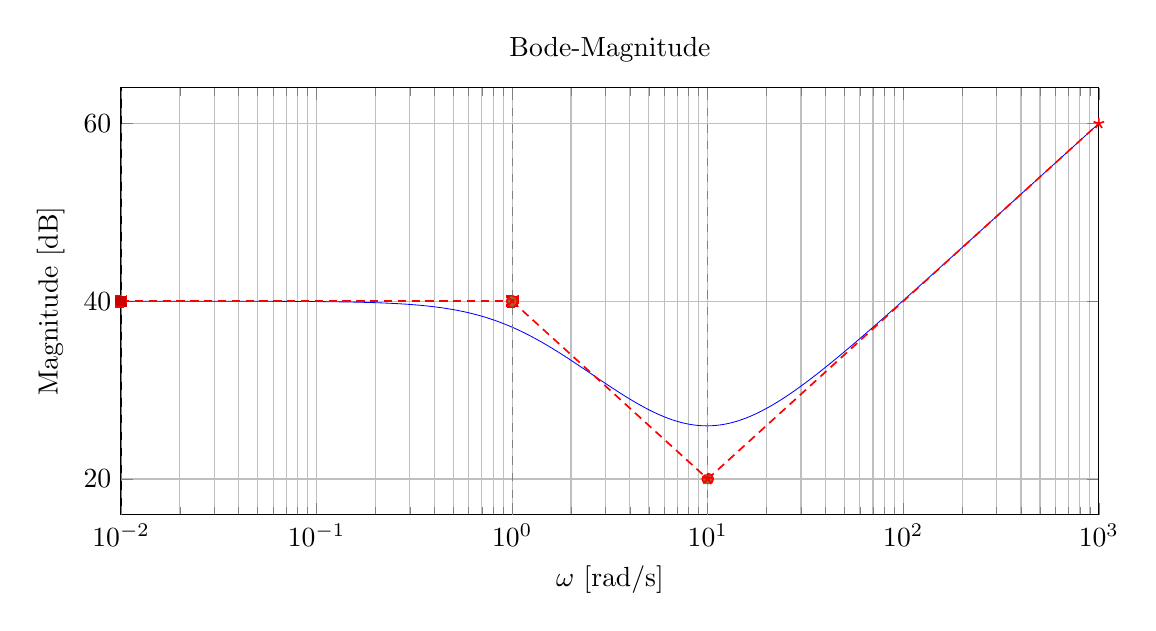
\begin{tikzpicture}
\begin{semilogxaxis}[
  width=14cm,height=7cm,
  xmin=1e-2,xmax=1e3,
  xlabel={$\omega$ [rad/s]},
  ylabel={Magnitude [dB]},
  grid=both,
  ytick distance=20,
  title={Bode-Magnitude}
]
\addplot[
  domain=1e-2:1e3,
  samples=600,
  mark=none,
  line width=0.3pt,
  blue
] {40*ln(sqrt(100 + x^2))/ln(10) - 20*ln(sqrt(1 + x^2))/ln(10)};
\addplot+[domain=1e-2:1,samples=2,dashed,dash pattern=on 3pt off 2pt,line width=0.6pt,red] {40};
\addplot+[domain=1:1e1,samples=2,dashed,dash pattern=on 3pt off 2pt,line width=0.6pt,red] {40 - 20*ln(x)/ln(10)};
\addplot+[domain=1e1:1e3,samples=2,dashed,dash pattern=on 3pt off 2pt,line width=0.6pt,red] {20 + 20*ln(x/10)/ln(10)};
\draw[gray,dashed] (rel axis cs:0,0) -- (rel axis cs:0,1);
\draw[gray,dashed] (axis cs:1,\pgfkeysvalueof{/pgfplots/ymin}) -- (axis cs:1,\pgfkeysvalueof{/pgfplots/ymax});
\draw[gray,dashed] (axis cs:10,\pgfkeysvalueof{/pgfplots/ymin}) -- (axis cs:10,\pgfkeysvalueof{/pgfplots/ymax});
\node[gray,anchor=south east] at (axis cs:1,\pgfkeysvalueof{/pgfplots/ymax}) {\scriptsize Pol $\omega_p=1$};
\node[gray,anchor=south east] at (axis cs:10,\pgfkeysvalueof{/pgfplots/ymax}) {\scriptsize Nullstellen $\omega_z=10$ (LHP \& RHP)};
\end{semilogxaxis}
\end{tikzpicture}
\vspace{6mm}
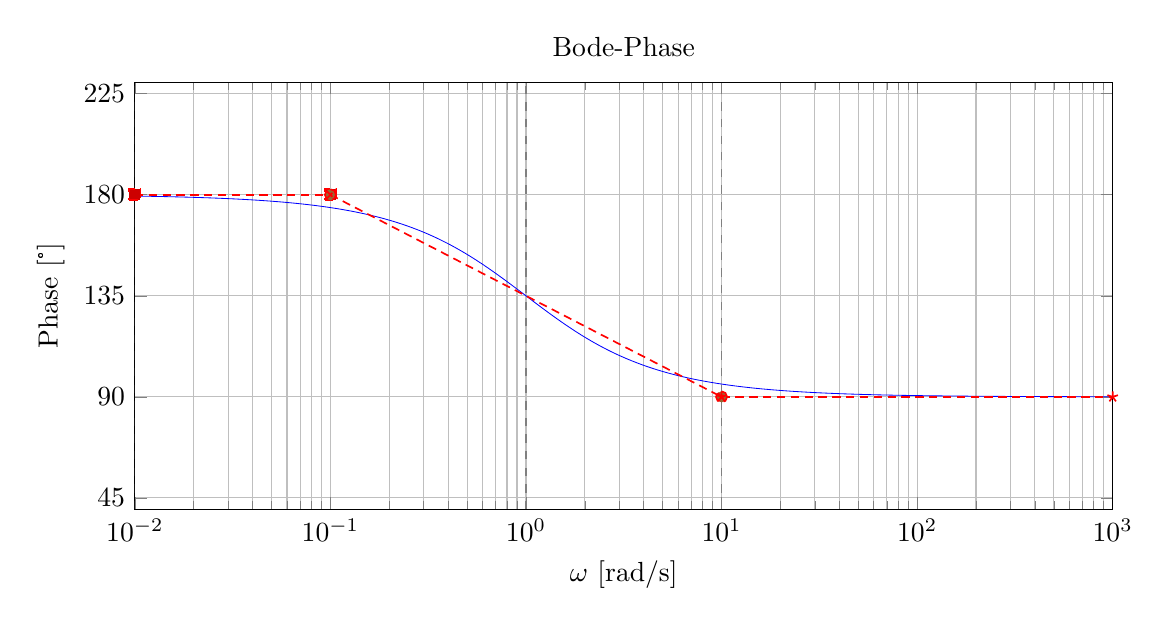
\begin{tikzpicture}
\begin{semilogxaxis}[
  width=14cm,height=7cm,
  xmin=1e-2,xmax=1e3,
  ytick distance=45,
  ymin=40,ymax=230,
  xlabel={$\omega$ [rad/s]},
  ylabel={Phase [°]},
  grid=both,
  title={Bode-Phase}
]
\addplot[
  domain=1e-2:1e3,
  samples=600,
  mark=none,
  line width=0.3pt,
  blue
] {180 - atan(x)};
\addplot+[domain=1e-2:1e-1,samples=2,dashed,dash pattern=on 3pt off 2pt,line width=0.6pt,red] {180};
\addplot+[domain=1e-1:1e1,samples=2,dashed,dash pattern=on 3pt off 2pt,line width=0.6pt,red] {135 - 45*ln(x)/ln(10)};
\addplot+[domain=1e1:1e3,samples=2,dashed,dash pattern=on 3pt off 2pt,line width=0.6pt,red] {90};
\draw[gray,dashed] (rel axis cs:0,0) -- (rel axis cs:0,1);
\draw[gray,dashed] (axis cs:1,\pgfkeysvalueof{/pgfplots/ymin}) -- (axis cs:1,\pgfkeysvalueof{/pgfplots/ymax});
\draw[gray,dashed] (axis cs:10,\pgfkeysvalueof{/pgfplots/ymin}) -- (axis cs:10,\pgfkeysvalueof{/pgfplots/ymax});
\node[gray,anchor=south east] at (axis cs:1,\pgfkeysvalueof{/pgfplots/ymax}) {\scriptsize Pol $\omega_p=1$};
\node[gray,anchor=south east] at (axis cs:10,\pgfkeysvalueof{/pgfplots/ymax}) {\scriptsize Nullstellen $\omega_z=10$ (LHP \& RHP)};
\end{semilogxaxis}
\end{tikzpicture}
\end{center}
\newpage

\subsection{Erklärung}
\begin{description}[leftmargin=1.2em,labelsep=.6em,font=\bfseries]

\item[1. Normalform herstellen.]
\[
H(s)=\frac{(s-10)(s+10)}{s+1}
=-100\,(1-sT_{z1})\,(1+sT_{z2})\cdot\frac{1}{1+sT_p}
\]
mit
\[
K_0=-100,\quad r=0,\quad T_{z1}=\tfrac{1}{10},\quad T_{z2}=\tfrac{1}{10},\quad T_p=1.
\]
\[
\underline{F}_1(s)=\bigl(1-sT_{z1}\bigr)\ \text{(RHP-Nullstelle)},\]
\[\underline{F}_2(s)=\bigl(1+sT_{z2}\bigr)\ \text{(LHP-Nullstelle)},\]
\[\underline{F}_3(s)=\tfrac{1}{1+sT_p}\ \text{(Pol)}.\]

\item[2. Eckfrequenzen bestimmen und sortieren.]
\[
\omega_{p}=1\,\mathrm{rad/s},\qquad
\omega_{z1}=\omega_{z2}=10\,\mathrm{rad/s},\qquad
\omega_p<\omega_z.
\]

\item[3. Startpunkt des Amplitudengangs festlegen (Geradennäherung).]
Setze \(\omega_{\min}=\omega_p=1\).
\[
F_{\mathrm{dB}}(\omega_{\min})=20\log_{10}\!\big(|K_0\underline{F}_{ges}^*(0)|\,\omega_{\min}^{\,r}\big)=20\log_{10}100=40\,\mathrm{dB}.
\]
Ankerpunkt: \(40\,\mathrm{dB}\) bei \(\omega=1\).

\item[4. Verlauf links vom Startpunkt zeichnen.]
Für \(\omega<1\) horizontale Asymptote bei \(40\,\mathrm{dB}\) (Anfangssteigung \(r\cdot 20\,\mathrm{dB/dec}=0\)). Waagrechte Gerade links von der kleinsten Eckfrequenz eintragen.

\item[5. Steigungswechsel an den Eckfrequenzen eintragen.]
Ab \(\omega=1\): Pol \(\Rightarrow\) Steigungswechsel \(-20\,\mathrm{dB/dec}\).
Ab \(\omega=10\): zwei Nullstellen \(\Rightarrow\) zusätzl. \(+40\,\mathrm{dB/dec}\).
Netto:
\[
\begin{cases}
40\,\mathrm{dB},& \omega<1,\\
40-20\log_{10}\omega,& 1\le\omega<10,\\
20+20\log_{10}(\omega/10),& \omega\ge 10.
\end{cases}
\]

\item[6. Eckabrundungen korrekt berücksichtigen.]
Einfacher Pol bei \(\omega=1\): \(-3\,\mathrm{dB}\) am Knick \(\Rightarrow |H(j1)|_{\mathrm{dB}}\approx 40-3=37\,\mathrm{dB}\).
Zwei Nullstellen bei \(\omega=10\): \(+6\,\mathrm{dB}\) am Knick \(\Rightarrow |H(j10)|_{\mathrm{dB}}\approx 20+6=26\,\mathrm{dB}\).

\item[7. Phasenstartwert festlegen.]
Verwende die Regel für $K_0\underline{F}_{ges}^*(0) <0$:
\[
\varphi(0)=-180^\circ + r\cdot 90^\circ= -180^\circ
\]
(Darstellung im Plot um \(+360^\circ\) verschoben \(\Rightarrow\) Start bei \(+180^\circ\)).

\item[8. Phasenänderung durch Pol und Nullstellen eintragen.]
Pol bei \(\omega_p\) bewirkt eine Phasenänderung \(-90^\circ\) über \([0.1,10]\).
Nullstellen bei \(\omega_z\): LHP-Nullstelle \(+90^\circ\) und RHP-Nullstelle \(-90^\circ\), beide über \([1,100]\). die \(+90^\circ\) und \(-90^\circ\) der beiden Nullstellen kompensieren sich zu \(0^\circ\). Netto wirkt in $[1,10]$ nur der Pol.
Näherung (mit Phasenverschiebung um \(+360^\circ\) gezeigt):
\[
\varphi(\omega)\approx
\begin{cases}
180^\circ,& \omega\le 0.1,\\
135^\circ-45^\circ\log_{10}\omega,& 0.1<\omega<10,\\
90^\circ,& \omega\ge 10.
\end{cases}
\]

\item[9. Grenzwerte und Konsistenz prüfen.]
DC: \(|H(0)|=100\Rightarrow 40\,\mathrm{dB}\); \(\varphi(0)=-180^\circ\) (gezeigt als \(+180^\circ\)).
HF: \(|H(j\omega)|\sim \omega^2/\omega= \omega \Rightarrow 20\log_{10}\omega + 20\,\mathrm{dB}\).

\end{description}

\subsubsection*{Stückweise Näherungen (für die Skizze)}
\[
|H(j\omega)|_{\mathrm{dB}}\approx
\begin{cases}
40,& \omega\ll 1,\\[2pt]
40-3,& \omega=1,\\[2pt]
40-20\log_{10}\omega,& 1\ll\omega\ll 10,\\[2pt]
20+6,& \omega=10,\\[2pt]
20+20\log_{10}(\omega/10),& \omega\gg 10,
\end{cases}
\]
\[
\varphi(\omega)\ (\text{Darstellung }+360^\circ)\approx
\begin{cases}
180^\circ,& \omega\le 0.1,\\[2pt]
135^\circ-45^\circ\log_{10}\omega,& 0.1<\omega<10,\\[2pt]
90^\circ,& \omega\ge 10.
\end{cases}
\]

\newpage
\section{}
\[
H(s)=\frac{10\sqrt{202}\,s}{(s+1)(s+10)}\,.
\]
\subsection{Bode-Diagramm}
\begin{center}
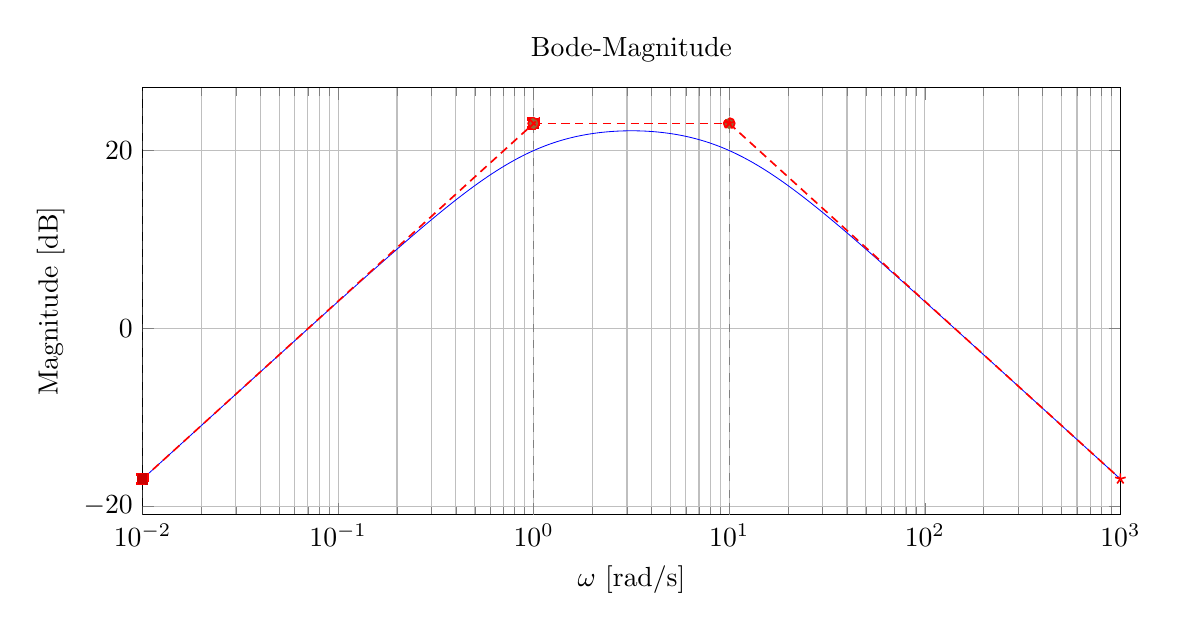
\begin{tikzpicture}
\begin{semilogxaxis}[
  width=14cm,height=7cm,
  xmin=1e-2,xmax=1e3,
  xlabel={$\omega$ [rad/s]},
  ylabel={Magnitude [dB]},
  ytick distance=20,
  grid=both,
  title={Bode-Magnitude}
]
\addplot[
  domain=1e-2:1e3,
  samples=600,
  mark=none,
  line width=0.3pt,
  blue
] {20 + 10*ln(202)/ln(10) + 20*ln(x)/ln(10) - 20*ln(sqrt(1 + x^2))/ln(10) - 20*ln(sqrt(100 + x^2))/ln(10)};
\addplot+[domain=1e-2:1,samples=2,dashed,dash pattern=on 3pt off 2pt,line width=0.6pt,red] {10*ln(202)/ln(10) + 20*ln(x)/ln(10)};
\addplot+[domain=1:1e1,samples=2,dashed,dash pattern=on 3pt off 2pt,line width=0.6pt,red] {10*ln(202)/ln(10)};
\addplot+[domain=1e1:1e3,samples=2,dashed,dash pattern=on 3pt off 2pt,line width=0.6pt,red] {10*ln(202)/ln(10) - 20*ln(x/10)/ln(10)};
\draw[gray,dashed] (rel axis cs:0,0) -- (rel axis cs:0,1);
\draw[gray,dashed] (axis cs:1,\pgfkeysvalueof{/pgfplots/ymin}) -- (axis cs:1,\pgfkeysvalueof{/pgfplots/ymax});
\draw[gray,dashed] (axis cs:10,\pgfkeysvalueof{/pgfplots/ymin}) -- (axis cs:10,\pgfkeysvalueof{/pgfplots/ymax});
\node[gray,anchor=south east] at (axis cs:1,\pgfkeysvalueof{/pgfplots/ymax}) {\scriptsize Pol $\omega_{p1}=1$};
\node[gray,anchor=south east] at (axis cs:10,\pgfkeysvalueof{/pgfplots/ymax}) {\scriptsize Pol $\omega_{p2}=10$};
\end{semilogxaxis}
\end{tikzpicture}
\vspace{6mm}
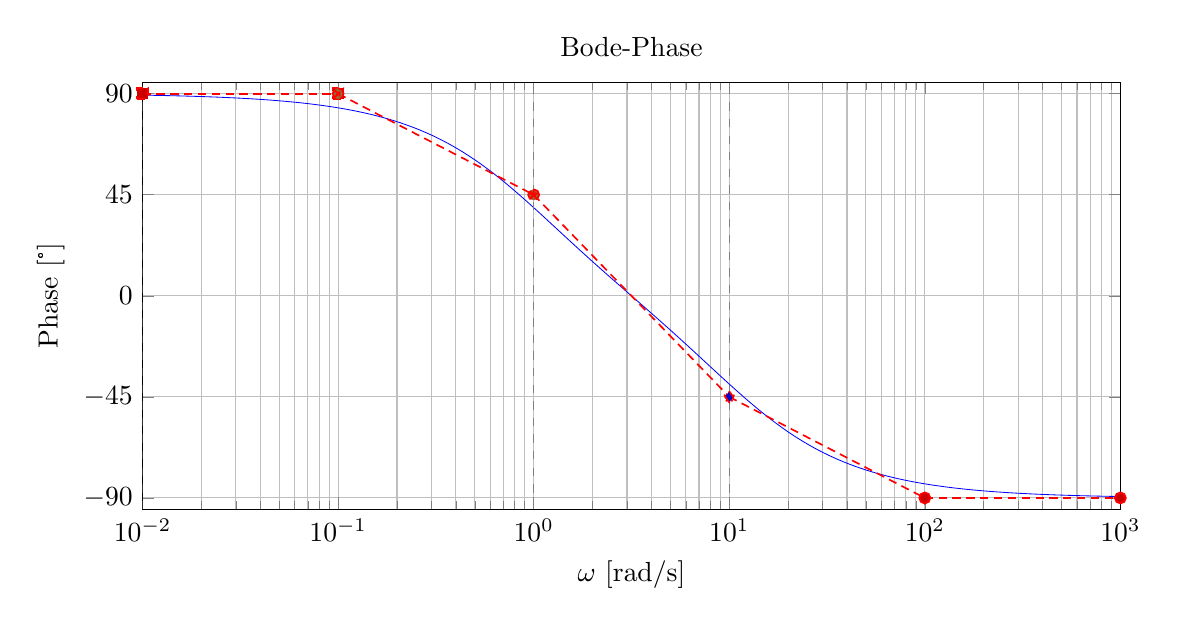
\begin{tikzpicture}
\begin{semilogxaxis}[
  width=14cm,height=7cm,
  xmin=1e-2,xmax=1e3,
  ymin=-95,ymax=95,
  ytick distance=45,
  xlabel={$\omega$ [rad/s]},
  ylabel={Phase [°]},
  grid=both,
  title={Bode-Phase}
]
\addplot[
  domain=1e-2:1e3,
  samples=600,
  mark=none,
  line width=0.3pt,
  blue
] {90 - atan(x) - atan(x/10)};
\addplot+[domain=1e-2:1e-1,samples=2,dashed,dash pattern=on 3pt off 2pt,line width=0.6pt,red] {90};
\addplot+[domain=1e-1:1e0,samples=2,dashed,dash pattern=on 3pt off 2pt,line width=0.6pt,red] {45 - 45*ln(x)/ln(10)};
\addplot+[domain=1e0:1e1,samples=2,dashed,dash pattern=on 3pt off 2pt,line width=0.6pt,red]{45 - 90*ln(x)/ln(10)};
\addplot+[domain=1e1:1e2,samples=2,dashed,dash pattern=on 3pt off 2pt,line width=0.6pt,red]{-45 - 45*ln(x/10)/ln(10)}; % bei 10: -45°, bei 100: -90°

\addplot+[domain=1e2:1e3,samples=2,dashed,dash pattern=on 3pt off 2pt,line width=0.6pt,red] {-90};
\draw[gray,dashed] (rel axis cs:0,0) -- (rel axis cs:0,1);
\draw[gray,dashed] (axis cs:1,\pgfkeysvalueof{/pgfplots/ymin}) -- (axis cs:1,\pgfkeysvalueof{/pgfplots/ymax});
\draw[gray,dashed] (axis cs:10,\pgfkeysvalueof{/pgfplots/ymin}) -- (axis cs:10,\pgfkeysvalueof{/pgfplots/ymax});
\node[gray,anchor=south east] at (axis cs:1,\pgfkeysvalueof{/pgfplots/ymax}) {\scriptsize Pol $\omega_{p1}=1$};
\node[gray,anchor=south east] at (axis cs:10,\pgfkeysvalueof{/pgfplots/ymax}) {\scriptsize Pol $\omega_{p2}=10$};
\end{semilogxaxis}
\end{tikzpicture}
\end{center}
\newpage
\subsection{Erklärung (ausführlich)}
\begin{description}[leftmargin=1.2em,labelsep=.6em,font=\bfseries]

\item[1. Normalform herstellen.]
\[
H(s)=\frac{10\sqrt{202}\,s}{(s+1)(s+10)}
= K_0\cdot s^{\,r}\cdot \frac{1}{(1+sT_{p1})(1+sT_{p2})}
\]
mit
\[
K_0=\sqrt{202},\quad r=1,\quad T_{p1}=1,\quad T_{p2}=\tfrac{1}{10}.
\]
\[
\underline{F}_1(s)=\frac{1}{1+sT_{p1}}=\frac{1}{1+s},\qquad
\underline{F}_2(s)=\frac{1}{1+sT_{p2}}=\frac{1}{1+\tfrac{s}{10}}
\]

\item[2. Eckfrequenzen bestimmen und sortieren.]
\[
\omega_{p1}=\frac{1}{T_{p1}}=1\,\mathrm{rad/s},\qquad
\omega_{p2}=\frac{1}{T_{p2}}=10\,\mathrm{rad/s},\qquad
\omega_{p1}<\omega_{p2}.
\]

\item[3. Startpunkt des Amplitudengangs festlegen (Geradennäherung).]
Setze \(\omega_{\min}=\omega_{p1}=1\).
\[
F_{\mathrm{dB}}(\omega_{\min})
=20\log_{10}\!\Big(|K_0\underline{F}_{ges}^*(0)|\,\omega_{\min}^{\,r}\Big)
=20\log_{10}(\sqrt{202}\cdot 1) \approx 23\,\mathrm{dB}.
\]
Ankerpunkt: \(23\,\mathrm{dB}\) bei \(\omega=1\).

\item[4. Verlauf links vom Startpunkt zeichnen.]
Für \(\omega<1\): Anfangssteigung \(r\cdot 20=+20\,\mathrm{dB/dec}\). Zeichne links vom Startpunkt die Gerade mit \(+20\,\mathrm{dB/dec}\) durch den Ankerpunkt.

\item[5. Steigungswechsel an den Eckfrequenzen eintragen.]
Pol bei \(\omega_{p1}=1\): Steigungsänderung \(-20\,\mathrm{dB/dec}\) \(\Rightarrow\) Netto \(0\,\mathrm{dB/dec}\) in \([1,10]\) (betragsflach).
Pol bei \(\omega_{p2}=10\): weitere \(-20\,\mathrm{dB/dec}\) \(\Rightarrow\) Netto \(-20\,\mathrm{dB/dec}\) für \(\omega\gg10\).
Geradennäherung:
\[
|H(j\omega)|_{\mathrm{dB}}\approx
\begin{cases}
10\log_{10}202+20\log_{10}\omega,& \omega\le 1,\\
10\log_{10}202,& 1<\omega\le 10,\\
10\log_{10}202-20\log_{10}(\omega/10),& \omega\ge 10.
\end{cases}
\]

\item[6. Eckabrundungen korrekt berücksichtigen.]
Jeder einfache Pol: \(-3\,\mathrm{dB}\) unter der Geradennäherung am Knick.
\[
|H(j1)|_{\mathrm{dB}}\approx 10\log_{10}202-3\ \mathrm{dB}\ \ (\approx 20\,\mathrm{dB}),\]\[
|H(j10)|_{\mathrm{dB}}\approx 10\log_{10}202-3\ \mathrm{dB}\ \ (\approx 20\,\mathrm{dB}).
\]

\item[7. Phasenstartwert festlegen.]
Verwende die Regel für $K_0\underline{F}_{ges}^*(0) > 0$
\[
\varphi(0)= r\cdot 90^\circ = 1\cdot 90^\circ = +90^\circ.
\]

\item[8. Phasenänderung durch die Polglieder eintragen.]
Nullstelle im Ursprung liefert konstant \(+90^\circ\). Pol bei \(1\): \(-90^\circ\) über \([0.1,10]\). Pol bei \(10\): \(-90^\circ\) über \([1,100]\). In \([1,10]\) überlappen sich beide Polbeiträge und addieren sich (Netto-Steilheit = Summe der Einzelsteilheiten). Näherung:
\[
\varphi(\omega)\approx
\begin{cases}
+90^\circ,& \omega\le 0.1,\\
45^\circ-45^\circ\log_{10}\omega + 90^\circ,& 0.1<\omega<1,\\
45^\circ-90^\circ\log_{10}\omega + 90^\circ,& 1<\omega<10,\\
-45^\circ-45^\circ\log_{10}(\omega/10),& 10<\omega<100,\\
-90^\circ,& \omega\ge 100.
\end{cases}
\]
(vereinfacht im Plot als \(90- \arctan\omega - \arctan(\omega/10)\) gezeigt; Grenzwert \(\varphi(\infty)=-90^\circ\)).

\item[9. Grenzwerte und Konsistenz prüfen.]
DC: \(|H(0)|=0\Rightarrow -\infty\,\mathrm{dB}\), \(\varphi(0)=+90^\circ\).
HF: \(|H(j\omega)|\sim \sqrt{202}\,\frac{\omega}{\omega^2/10}= \sqrt{202}\cdot \frac{10}{\omega}\Rightarrow 10\log_{10}202-20\log_{10}(\omega/10)\,\mathrm{dB}\), \(\varphi(\infty)=+90^\circ-180^\circ=-90^\circ\).
Pol-/Nullzählung: \(m=1\), \(n=2\Rightarrow (m-n)\cdot 90^\circ=-90^\circ\) konsistent.

\end{description}

\subsubsection*{Stückweise Näherungen (für die Skizze)}
\[
|H(j\omega)|_{\mathrm{dB}}\approx
\begin{cases}
10\log_{10}202+20\log_{10}\omega,& \omega\ll 1,\\[2pt]
10\log_{10}202-3,& \omega=1,\\[2pt]
10\log_{10}202,& 1\ll\omega\ll 10,\\[2pt]
10\log_{10}202-3,& \omega=10,\\[2pt]
10\log_{10}202-20\log_{10}(\omega/10),& \omega\gg 10,
\end{cases}
\]\[
\varphi(\omega)\approx
\begin{cases}
+90^\circ,& \omega\le 0.1,\\[2pt]
45^\circ-45^\circ\log_{10}\omega + 90^\circ,& 0.1<\omega<1,\\[2pt]
45^\circ-90^\circ\log_{10}\omega + 90^\circ,& 1<\omega<10,\\[2pt]
-45^\circ-45^\circ\log_{10}(\omega/10),& 10<\omega<100,\\[2pt]
-90^\circ,& \omega\ge 100.
\end{cases}
\]

\newpage
\section{}
\[
H(s)=\frac{s\,(0.1 - s)\,(s+10)}{(s+1)^2}\,.
\]
\subsection{Bode-Diagramm}
\begin{center}
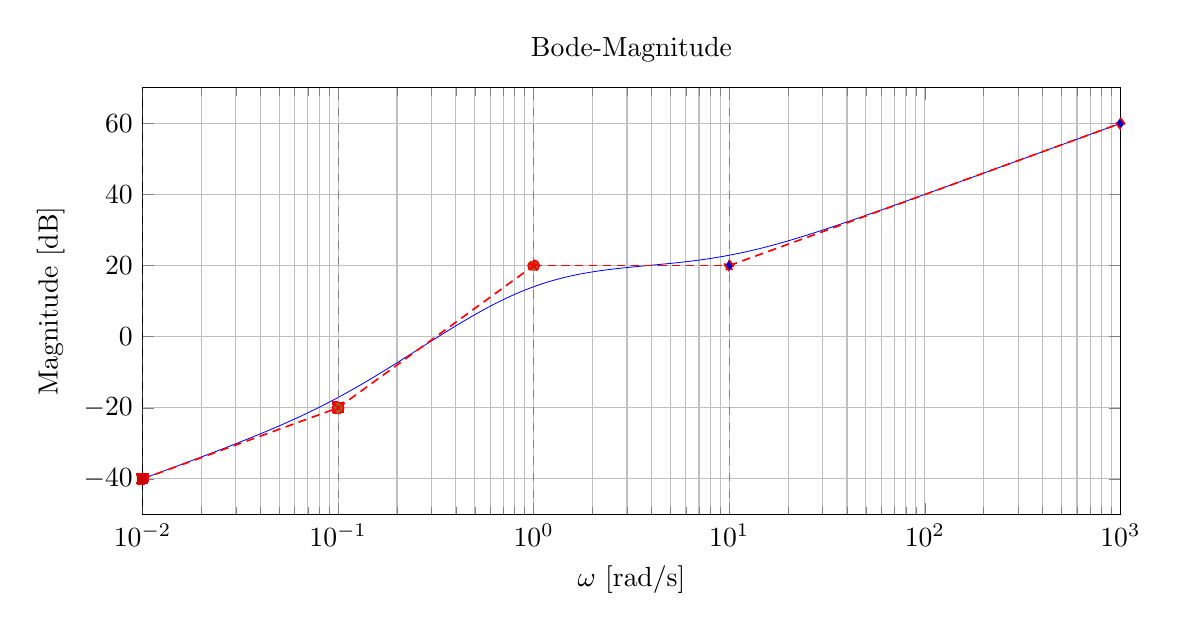
\begin{tikzpicture}
\begin{semilogxaxis}[
  width=14cm,height=7cm,
  ytick distance=20,
  xmin=1e-2,xmax=1e3,
  xlabel={$\omega$ [rad/s]},
  ylabel={Magnitude [dB]},
  grid=both,
  title={Bode-Magnitude}
]
\addplot[
  domain=1e-2:1e3,
  samples=800,
  mark=none,
  line width=0.3pt,
  blue
] {20*ln(x)/ln(10)
   +20*ln(sqrt(1 + (x/0.1)^2))/ln(10)
   +20*ln(sqrt(1 + (x/10)^2))/ln(10)
   -40*ln(sqrt(1 + x^2))/ln(10)};
\addplot+[domain=1e-2:1e-1,samples=2,dashed,dash pattern=on 3pt off 2pt,line width=0.6pt,red] {20*ln(x)/ln(10)};
\addplot+[domain=1e-1:1,samples=2,dashed,dash pattern=on 3pt off 2pt,line width=0.6pt,red] {40*ln(x)/ln(10) + 20};
\addplot+[domain=1:1e1,samples=2,dashed,dash pattern=on 3pt off 2pt,line width=0.6pt,red] {20};
\addplot+[domain=1e1:1e3,samples=2,dashed,dash pattern=on 3pt off 2pt,line width=0.6pt,red] {20 + 20*ln(x/10)/ln(10)};
\draw[gray,dashed] (rel axis cs:0,0) -- (rel axis cs:0,1);
\draw[gray,dashed] (axis cs:0.1,\pgfkeysvalueof{/pgfplots/ymin}) -- (axis cs:0.1,\pgfkeysvalueof{/pgfplots/ymax});
\draw[gray,dashed] (axis cs:1,\pgfkeysvalueof{/pgfplots/ymin}) -- (axis cs:1,\pgfkeysvalueof{/pgfplots/ymax});
\draw[gray,dashed] (axis cs:10,\pgfkeysvalueof{/pgfplots/ymin}) -- (axis cs:10,\pgfkeysvalueof{/pgfplots/ymax});
\node[gray,anchor=south east] at (axis cs:0.1,\pgfkeysvalueof{/pgfplots/ymax}) {\scriptsize Nullstelle $\omega_z=0.1$ (RHP)};
\node[gray,anchor=south east] at (axis cs:1,\pgfkeysvalueof{/pgfplots/ymax}) {\scriptsize Pol $\omega_p=1$ (doppelt)};
\node[gray,anchor=south east] at (axis cs:10,\pgfkeysvalueof{/pgfplots/ymax}) {\scriptsize Nullstelle $\omega_z=10$};
\end{semilogxaxis}
\end{tikzpicture}
\vspace{6mm}
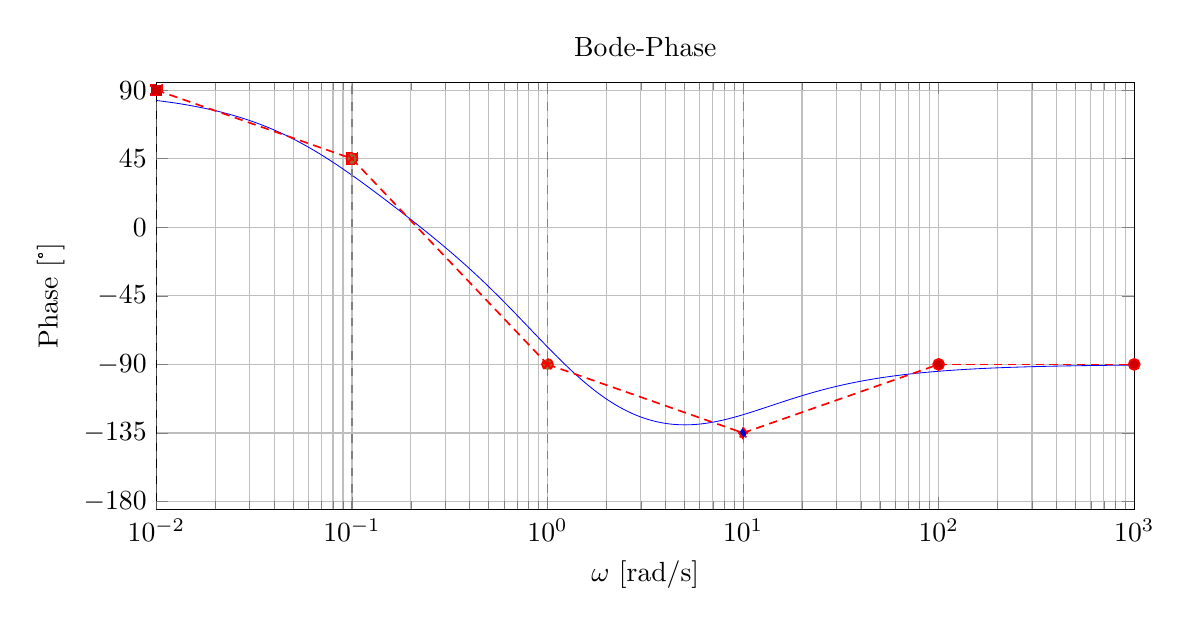
\begin{tikzpicture}
\begin{semilogxaxis}[
  width=14cm,height=7cm,
  xmin=1e-2,xmax=1e3,
  ytick distance=45,
  ymin=-185,ymax=95,
  xlabel={$\omega$ [rad/s]},
  ylabel={Phase [°]},
  grid=both,
  title={Bode-Phase}
]
\addplot[
  domain=1e-2:1e3,
  samples=800,
  mark=none,
  line width=0.3pt,
  blue
] {90 - atan(x/0.1) + atan(x/10) - 2*atan(x)};
\addplot+[domain=1e-2:1e-1,samples=2,dashed,dash pattern=on 3pt off 2pt,line width=0.6pt,red] {45 - 45*ln(x/0.1)/ln(10)};
\addplot+[domain=1e-1:1e0,samples=2,dashed,dash pattern=on 3pt off 2pt,line width=0.6pt,red] {45 - 135*ln(x/0.1)/ln(10)};
\addplot+[domain=1e0:1e1,samples=2,dashed,dash pattern=on 3pt off 2pt,line width=0.6pt,red] {-90 - 45*ln(x)/ln(10)};
\addplot+[domain=1e1:1e2,samples=2,dashed,dash pattern=on 3pt off 2pt,line width=0.6pt,red] {-135 + 45*ln(x/10)/ln(10)};
\addplot+[domain=1e2:1e3,samples=2,dashed,dash pattern=on 3pt off 2pt,line width=0.6pt,red] {-90};
\draw[gray,dashed] (rel axis cs:0,0) -- (rel axis cs:0,1);
\draw[gray,dashed] (axis cs:0.1,\pgfkeysvalueof{/pgfplots/ymin}) -- (axis cs:0.1,\pgfkeysvalueof{/pgfplots/ymax});
\draw[gray,dashed] (axis cs:1,\pgfkeysvalueof{/pgfplots/ymin}) -- (axis cs:1,\pgfkeysvalueof{/pgfplots/ymax});
\draw[gray,dashed] (axis cs:10,\pgfkeysvalueof{/pgfplots/ymin}) -- (axis cs:10,\pgfkeysvalueof{/pgfplots/ymax});
\node[gray,anchor=south east] at (axis cs:0.1,\pgfkeysvalueof{/pgfplots/ymax}) {\scriptsize Nullstelle $\omega_z=0.1$ (RHP)};
\node[gray,anchor=south east] at (axis cs:1,\pgfkeysvalueof{/pgfplots/ymax}) {\scriptsize Pol $\omega_p=1$ (doppelt)};
\node[gray,anchor=south east] at (axis cs:10,\pgfkeysvalueof{/pgfplots/ymax}) {\scriptsize Nullstelle $\omega_z=10$};
\end{semilogxaxis}
\end{tikzpicture}
\end{center}
\newpage

\subsection{Erklärung}
\begin{description}[leftmargin=1.2em,labelsep=.6em,font=\bfseries]

\item[1. Normalform herstellen.]
Bringe die Übertragungsfunktion in die Standardform.
\[
H(s)=K_0\cdot s^{\,r}\,(1-sT_{z1})\,(1+sT_{z2})\cdot\frac{1}{(1+sT_p)^2}
\]
mit
\[
K_0=1,\quad r=1,\quad T_{z1}=10,\quad T_{z2}=0.1,\quad T_p=1.
\]

\[\underline{F}_2(s)=(1-sT_{z1})\ \text{(RHP-Nullstelle)},\quad\]
\[\underline{F}_3(s)=(1+sT_{z2})\ \text{(LHP-Nullstelle)},\quad\]
\[\underline{F}_4(s)=\tfrac{1}{(1+sT_p)^2}\ \text{(Doppelpol)}.\]


\item[2. Eckfrequenzen bestimmen und sortieren.]
\[
\omega_{z1}=\frac{1}{T_{z1}}=0.1 \,\mathrm{rad/s}\,,\quad \omega_{p}=\frac{1}{T_{p}}=1\,\mathrm{rad/s}\,\ \text{(doppelt)},\quad \omega_{z2}=\frac{1}{T_{z2}}=10\,\mathrm{rad/s}\,\] 
\[\omega_{zR}<\omega_{p}<\omega_{zL}
\]

\item[3. Startpunkt des Amplitudengangs festlegen (Geradennäherung).]
Setze \(\omega_{\min}=\omega_{zR}=0.1\).
\[
F_{\mathrm{dB}}(\omega_{\min})=20\log_{10}\!\Big(|K_0F^*_{\mathrm{ges}}(0)|\,\omega_{\min}^{\,r}\Big)
=20\log_{10}(0.1)=-20\,\mathrm{dB}.
\]
Ankerpunkt: \(-20\,\mathrm{dB}\) bei \(\omega=0.1\).

\item[4. Verlauf links vom Startpunkt zeichnen.]
Für \(\omega<0.1\) Anfangssteigung \(r\cdot 20=+20\,\mathrm{dB/dec}\) \(\Rightarrow\) Gerade mit \(+20\,\mathrm{dB/dec}\) durch den Ankerpunkt.

\item[5. Steigungswechsel an den Eckfrequenzen eintragen.]
Nullstelle bei \(0.1\): \(+20\,\mathrm{dB/dec}\) \(\Rightarrow\) Netto \(+40\,\mathrm{dB/dec}\) in \([0.1,1]\).
Doppelpol bei \(1\): \(-40\,\mathrm{dB/dec}\) \(\Rightarrow\) Netto \(0\,\mathrm{dB/dec}\) in \([1,10]\).
Nullstelle bei \(10\): \(+20\,\mathrm{dB/dec}\) \(\Rightarrow\) Netto \(+20\,\mathrm{dB/dec}\) für \(\omega\gg10\).
Geradennäherung:
\[
|H(j\omega)|_{\mathrm{dB}}\approx
\begin{cases}
20\log_{10}\omega,& \omega\le 0.1,\\
40\log_{10}\omega+20,& 0.1<\omega\le 1,\\
20,& 1<\omega\le 10,\\
20+20\log_{10}(\omega/10),& \omega\ge 10.
\end{cases}
\]

\item[6. Eckabrundungen korrekt berücksichtigen.]
RHP-/LHP-Nullstelle: \(+3\,\mathrm{dB}\) am Knick (\(\omega=0.1\) bzw. \(10\)).
Doppelpol (\(\omega=1\)): \(-6\,\mathrm{dB}\) am Knick.

\item[7. Phasenstartwert festlegen.]
Da \(K_0\,F^*_{\mathrm{ges}}(0)>0\) und \(r=1\):
\[
\varphi(0)=0^\circ + r\cdot 90^\circ=+90^\circ.
\]

\item[8. Phasenänderung durch Nullstellen und Pol eintragen.]
Beiträge: RHP-Nullstelle \(-90^\circ\) über \([0.01,1]\); Doppelpol \(-180^\circ\) über \([0.1,10]\); LHP-Nullstelle \(+90^\circ\) über \([1,100]\).
Überlappungen addieren sich im jeweiligen Bereich (\([0.1,1]\) wirken RHP-Nullstelle und beide Pole gemeinsam; \([1,10]\) wirken beide Pole und die LHP-Nullstelle gemeinsam)).
Näherung:


\item[9. Grenzwerte und Konsistenz prüfen.]
DC: \(|H(0)|=0\Rightarrow -\infty\,\mathrm{dB}\), \(\varphi(0)=+90^\circ\).
HF: \(|H(j\omega)|\sim \omega\cdot \omega \cdot \omega / \omega^2=\omega \Rightarrow +\infty \,\mathrm{dB}\).
\end{description}

\subsubsection*{Stückweise Näherungen (für die Skizze)}
\[
|H(j\omega)|_{\mathrm{dB}}\approx
\begin{cases}
20\log_{10}\omega,& \omega\ll 0.1,\\[2pt]
40\log_{10}\omega+20,& 0.1\ll\omega\ll 1,\\[2pt]
20,& 1\ll\omega\ll 10,\\[2pt]
20+20\log_{10}(\omega/10),& \omega\gg 10,
\end{cases}
\]
\[
\varphi(\omega)\approx
\begin{cases}
+90^\circ,& \omega\le 0.01,\\[2pt]
45^\circ-45^\circ\log_{10}(\omega/0.1),& 0.01<\omega<0.1,\\[2pt]
45^\circ-135^\circ\log_{10}(\omega/0.1),& 0.1<\omega<1,\\[2pt]
-90^\circ-45^\circ\log_{10}\omega,& 1<\omega<10,\\[2pt]
-135^\circ+45^\circ\log_{10}(\omega/10),& 10<\omega<100,\\[2pt]
-90^\circ,& \omega\ge 100.
\end{cases}
\]

\newpage
\section{}
\[
H(s)=\frac{1}{s}\,.
\]
\subsection{Bode-Diagramm}
\begin{center}
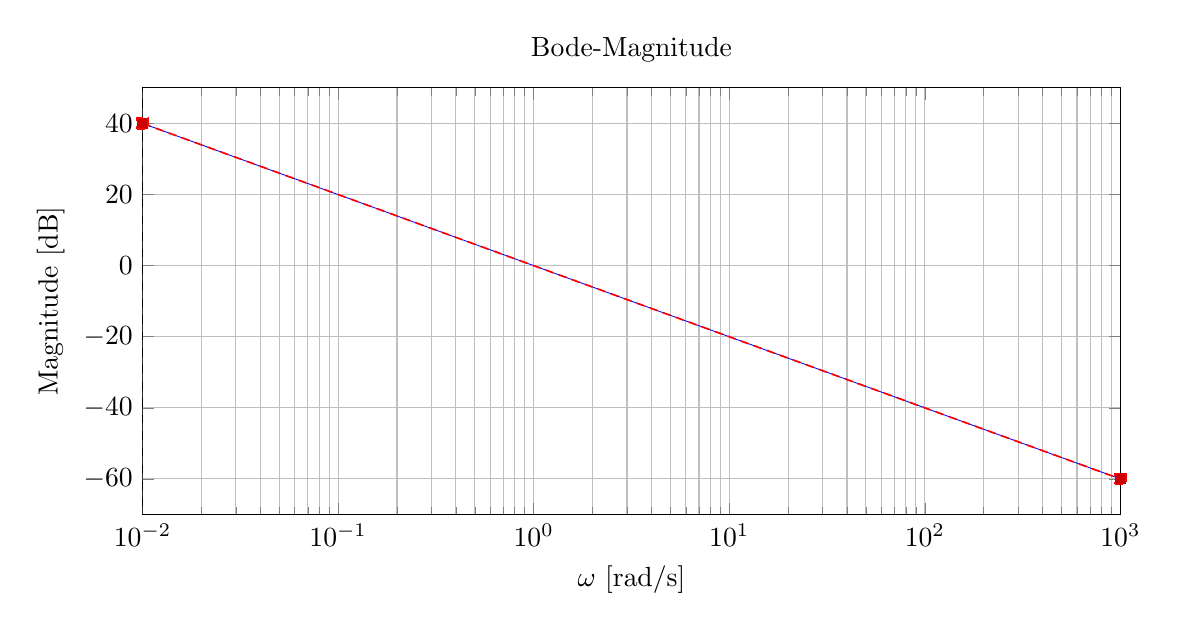
\begin{tikzpicture}
\begin{semilogxaxis}[
  width=14cm,height=7cm,
  ytick distance=20,
  xmin=1e-2,xmax=1e3,
  xlabel={$\omega$ [rad/s]},
  ylabel={Magnitude [dB]},
  grid=both,
  title={Bode-Magnitude}
]
\addplot[
  domain=1e-2:1e3,
  samples=400,
  mark=none,
  line width=0.3pt,
  blue
] {-20*ln(x)/ln(10)};
\addplot+[domain=1e-2:1e3,samples=2,dashed,dash pattern=on 3pt off 2pt,line width=0.6pt,red] {-20*ln(x)/ln(10)};
\draw[gray,dashed] (rel axis cs:0,0) -- (rel axis cs:0,1);
\end{semilogxaxis}
\end{tikzpicture}
\vspace{6mm}
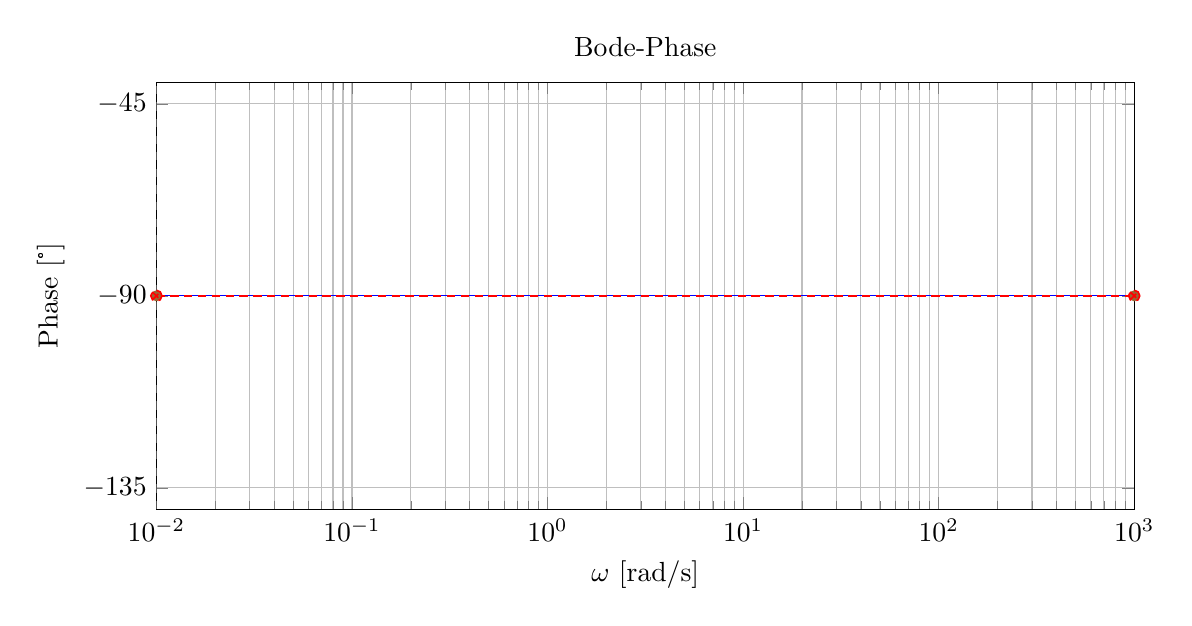
\begin{tikzpicture}
\begin{semilogxaxis}[
  width=14cm,height=7cm,
  xmin=1e-2,xmax=1e3,
  ymin=-140,ymax=-40,
  ytick distance=45,
  xlabel={$\omega$ [rad/s]},
  ylabel={Phase [°]},
  grid=both,
  title={Bode-Phase}
]
\addplot[
  domain=1e-2:1e-3,
  samples=2,
  mark=none,
  line width=0.3pt,
  blue
] {-90};
\addplot[
  domain=1e-3:1e3,
  samples=2,
  mark=none,
  line width=0.3pt,
  blue
] {-90};
\addplot+[domain=1e-2:1e3,samples=2,dashed,dash pattern=on 3pt off 2pt,line width=0.6pt,red] {-90};
\draw[gray,dashed] (rel axis cs:0,0) -- (rel axis cs:0,1);
\end{semilogxaxis}
\end{tikzpicture}
\end{center}
\newpage
\subsection{Erklärung (ausführlich)}
\begin{description}[leftmargin=1.2em,labelsep=.6em,font=\bfseries]

\item[1. Normalform herstellen.]
\[
H(s)=\frac{1}{s}=K_0\cdot s^{\,r},\qquad
K_0=1,\quad r=-1.
\]


\item[2. Eckfrequenzen bestimmen und sortieren.]
Keine endliche Eckfrequenz; nur Ursprungspol.

\item[3. Startpunkt des Amplitudengangs festlegen (Geradennäherung).]
Wähle Referenz \(\omega_{\mathrm{ref}}=1\,\mathrm{rad/s}\) (Fixpunkt).
\[
F_{\mathrm{dB}}(\omega_{\mathrm{ref}})=20\log_{10}\!\big(|K_0|\ \omega_{\mathrm{ref}}^{\,r}\big)
=20\log_{10}(1^{\,{-1}})=0\,\mathrm{dB}.
\]
Ankerpunkt: \(0\,\mathrm{dB}\) bei \(\omega=1\).

\item[4. Verlauf links vom Startpunkt zeichnen.]
Konstante Steigung \(r\cdot 20\,\mathrm{dB/dec} =-20\,\mathrm{dB/dec}\) über alle Frequenzen. Gerade durch den Ankerpunkt mit Steigung \(-20\,\mathrm{dB/dec}\).

\item[5. Steigungswechsel an den Eckfrequenzen eintragen.]
Kein Steigungswechsel (keine endliche Ecke).

\item[6. Eckabrundung korrekt berücksichtigen.]
Keine Ecken \(\Rightarrow\) keine \(\pm 3/6/9\,\mathrm{dB}\)-Korrekturen.

\item[7. Phasenstartwert festlegen.]
Da \(K_0\,F^*_{\mathrm{ges}}(0)>0\) und \(r=-1\):
\[
\varphi(0)=r\cdot 90^\circ = -90^\circ.
\]

\item[8. Phasenänderung durch Teilglieder eintragen.]
Nur Ursprungspol: Phase konstant \(-90^\circ\). Keine Überlappung, keine Addition weiterer Beiträge.

\item[9. Grenzwerte und Konsistenz prüfen.]
DC: \(|H(0)|\to\infty\Rightarrow +\infty\,\mathrm{dB}\), \(\varphi(0)=-90^\circ\).
HF: \(|H(j\omega)|=1/\omega\Rightarrow -20\log_{10}\omega\,\mathrm{dB}\), \(\varphi(\infty)=-90^\circ\).

\end{description}

\subsubsection*{Stückweise Näherungen (für die Skizze)}
\[
|H(j\omega)|_{\mathrm{dB}}\approx
\begin{cases}
-20\log_{10}\omega,& \omega\ll 1,\\[2pt]
0,& \omega=1,\\[2pt]
-20\log_{10}\omega,& \omega\gg 1,
\end{cases}
\]\[
\varphi(\omega)\approx -90^\circ\ \text{(für alle }\omega\text{)}.
\]

\newpage
\section{}
\[
H(s)=\frac{100}{s^2+s+100}\,.
\]
\subsection{Bode-Diagramm}
\begin{center}
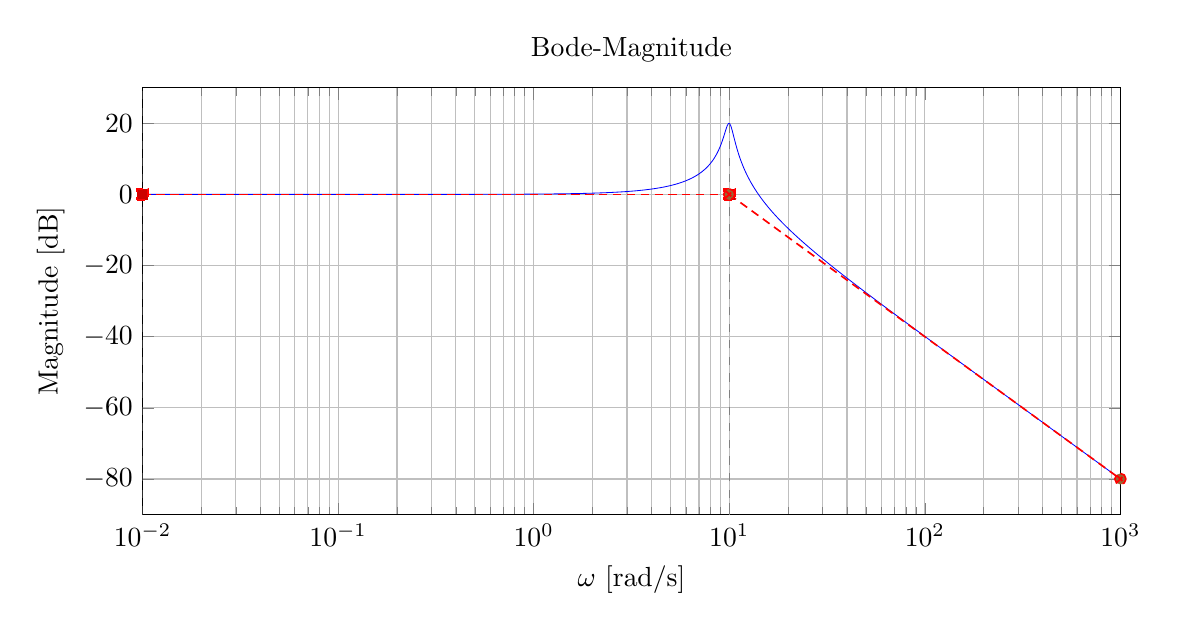
\begin{tikzpicture}
\begin{semilogxaxis}[
  width=14cm,height=7cm,
  xmin=1e-2,xmax=1e3,
  xlabel={$\omega$ [rad/s]},
  ylabel={Magnitude [dB]},
  ytick distance=20,
  grid=both,
  title={Bode-Magnitude}
]
\addplot[
  domain=1e-2:1e3,
  samples=800,
  mark=none,
  line width=0.3pt,
  blue
] {-10*ln((1 - (x/10)^2)^2 + (x/100)^2)/ln(10)};
\addplot+[domain=1e-2:1e1,samples=2,dashed,dash pattern=on 3pt off 2pt,line width=0.6pt,red] {0};
\addplot+[domain=1e1:1e3,samples=2,dashed,dash pattern=on 3pt off 2pt,line width=0.6pt,red] {-40*ln(x/10)/ln(10)};
\draw[gray,dashed] (rel axis cs:0,0) -- (rel axis cs:0,1);
\draw[gray,dashed] (axis cs:10,\pgfkeysvalueof{/pgfplots/ymin}) -- (axis cs:10,\pgfkeysvalueof{/pgfplots/ymax});
\node[gray,anchor=south east] at (axis cs:10,\pgfkeysvalueof{/pgfplots/ymax}) {\scriptsize Polpaar $\omega_n=10$, $\zeta=0.05$};
\end{semilogxaxis}
\end{tikzpicture}
\vspace{6mm}
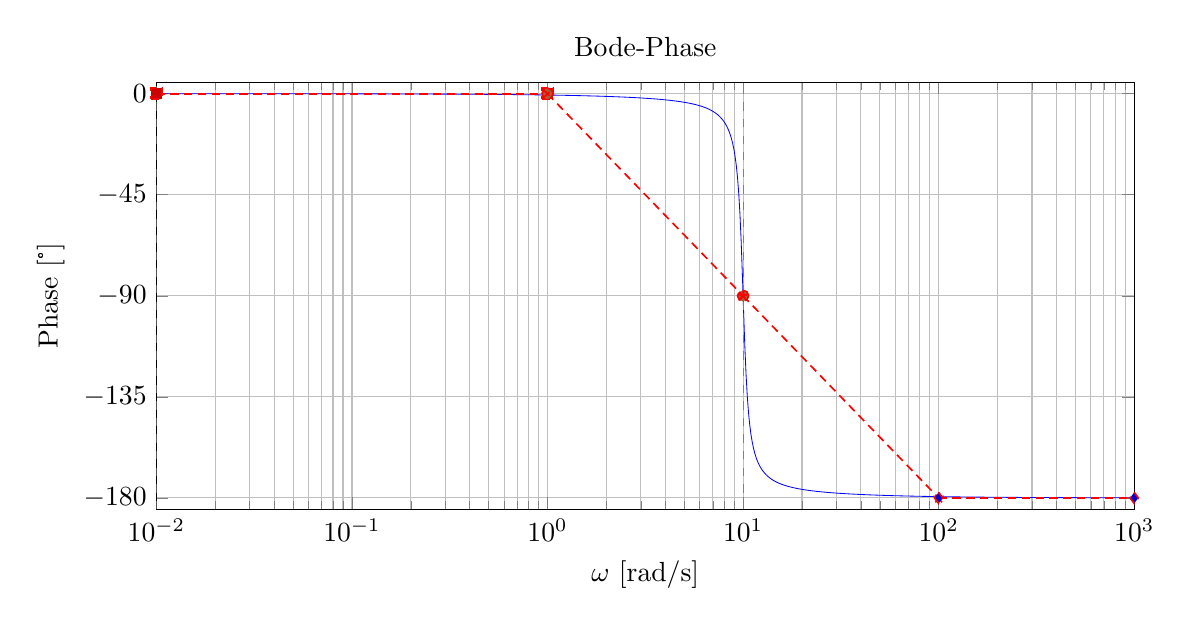
\begin{tikzpicture}
\begin{semilogxaxis}[
  width=14cm,height=7cm,
  xmin=1e-2,xmax=1e3,
  ymin=-185,ymax=5,
  ytick distance=45,
  xlabel={$\omega$ [rad/s]},
  ylabel={Phase [°]},
  grid=both,
  title={Bode-Phase}
]
\addplot[
  domain=1e-2:1e3,
  samples=800,
  mark=none,
  line width=0.3pt,
  blue
] {-atan2(x/100, 1 - (x/10)^2)};
\addplot+[domain=1e-2:1e0,samples=2,dashed,dash pattern=on 3pt off 2pt,line width=0.6pt,red] {0};
\addplot+[domain=1e0:1e1,samples=2,dashed,dash pattern=on 3pt off 2pt,line width=0.6pt,red] {-90*ln(x)/ln(10)};
\addplot+[domain=1e1:1e2,samples=2,dashed,dash pattern=on 3pt off 2pt,line width=0.6pt,red] {-90 - 90*ln(x/10)/ln(10)};
\addplot+[domain=1e2:1e3,samples=2,dashed,dash pattern=on 3pt off 2pt,line width=0.6pt,red] {-180};
\draw[gray,dashed] (rel axis cs:0,0) -- (rel axis cs:0,1);
\draw[gray,dashed] (axis cs:10,\pgfkeysvalueof{/pgfplots/ymin}) -- (axis cs:10,\pgfkeysvalueof{/pgfplots/ymax});
\node[gray,anchor=south east] at (axis cs:10,\pgfkeysvalueof{/pgfplots/ymax}) {\scriptsize Polpaar $\omega_n=10$, $\zeta=0.05$};
\end{semilogxaxis}
\end{tikzpicture}
\end{center}
\newpage
\subsection{Erklärung}
\begin{description}[leftmargin=1.2em,labelsep=.6em,font=\bfseries]

\item[1. Normalform herstellen.]
Bringe die Übertragungsfunktion exakt in die im Skript definierte Standardform für reelle Pol-/Nullstellen.
\[
H(s)=K_0\cdot s^{\,r}\cdot\frac{1}{1+2d_nT_{p}\cdot s + T_{p}^2\cdot s^2}
\quad.
\]
Hier haben wir: \[
\underline{F}_1(s)=\frac{1}{1+2d_nT_{p}\cdot s + T_{p}^2\cdot s^2},\quad K_0 = \frac{100}{100}=1,\]\[\quad T_p=\frac{1}{10}, \quad d_n=\frac{1}{20}\quad \text{und}\quad r = 0.
\]
\vspace{0.2cm}
Klassifizikation des ersten Teilglieds $\underline{F}_1$: konjugiertes komplexes Polpaar zweiter Ordnung.

\item[2. Eckfrequenz bestimmen und sortieren.]
Bestimme die Eckfrequenz aus der Normform:
\[
\omega_n=\frac{1}{T_p}=10\,\mathrm{rad/s}
\]
Es existiert nur diese charakteristische Frequenz; die aufsteigende Sortierung \(\omega_1<\omega_2<\dots\) ist damit trivial. 

\item[3. Startpunkt des Amplitudengangs festlegen (Geradennäherung).]
Setze die Startfrequenz gleich der kleinsten Eckfrequenz \(\omega_{\min}=\omega_n = 10\,\mathrm{rad/s}\). Verwende die Regel im Skript
\[
F_{\mathrm{dB}}(\omega_{\min})=20\log_{10}\!\Big(|K_0\,F^*_{ges}(0)|\cdot\,\omega_{\min}^{\,r}\Big) = 20 \log_{10}(1) = 0\,\mathrm{dB}.
\]
Dieser Punkt dient als Anker für die Geradennäherung (ohne Resonanzüberhöhung). 

\item[4. Verlauf links vom Startpunkt zeichnen.]
Für \(\omega<\omega_{\min}\) bleibt die Amplituden-Asymptote waagrecht, denn die Anfangssteigung beträgt \(r\cdot 20\,\mathrm{dB/dec}=0\). Trage also eine horizontale Linie bei \(0\,\mathrm{dB}\) ein. 

\item[5. Steigungswechsel an der Eckfrequenz eintragen.]
Ein konjugiertes Polpaar zweiter Ordnung reduziert die Steigung ab \(\omega_n\) um \(40\,\mathrm{dB/dec}\). Da bis jetzt die Steigung \(0\,\mathrm{dB/dec}\) betrug, ist diese ab jetzt \(-40\,\mathrm{dB/dec}\). Zeichne rechts von \(\omega_n\) die Gerade mit Steigung \(-40\,\mathrm{dB/dec}\). Die Formel für die Geradennäherung lautet:
\[
|H(j\omega)|_{\mathrm{dB}}\approx -40\log_{10}\!\Big(\frac{\omega}{\omega_n}\Big)\quad(\omega\ge \omega_n=10).
\]

\item[6. Eckabrundung korrekt berücksichtigen.]
Da $d_n \ll \tfrac{1}{2}$ müssen wir beim Abrunden eine Resonanzüberhöhung mit einbeziehen. Laut Skript erreicht der Magnitudengang bei $\omega = \omega_n$ eine Überhöhung von

\[
-20\log_{10}(2d_n)= -20\log_{10}(\tfrac{1}{10})=20\,\mathrm{dB}
\]
über der asymptotischen \(0\,\mathrm{dB}\)-Gerade. Trage dort einen Stützpunkt und runde die Ecke mit Resonanz entsprechend aus. 

\item[7. Phasenstartwert festlegen.]
Da \(K_0F_{ges}(0)>0\) und \(r=0\), ist der Startwert der Phase
\[
\varphi(0)=r\cdot90^\circ=0^\circ.
\]

\item[8. Phasenänderung durch das Polpaar eintragen.]
Ein komplexes Polpaar zweiter Ordnung erzeugt insgesamt eine Phasenänderung von \(-180^\circ\). Trage die Näherung ein:
\[
\varphi(\omega)\approx
\begin{cases}
0^\circ,& \omega\le 10^{-1}\omega_n\;(=1),\\
\text{linear }-90^\circ/\text{Dec},& 10^{-1}\omega_n<\omega<\omega_n,\\
\text{linear }-90^\circ/\text{Dec},& \omega_n<\omega<10\,\omega_n,\\
-180^\circ,& \omega\ge 10\,\omega_n\;(=100).
\end{cases}
\]
Das lineare Zwischenstück kann formelkonform als \(\varphi(\omega)\approx -90^\circ\log_{10}\omega\) in \([1,10]\) und \(\varphi(\omega)\approx -90^\circ-90^\circ\log_{10}(\omega/10)\) in \([10,100]\) dargestellt werden. 

\item[9. Grenzwerte und Konsistenz prüfen.]
DC: \(|H(0)|=1\Rightarrow 0\,\mathrm{dB}\), \(\varphi(0)=0^\circ\). HF: \(|H(j\omega)|\sim 100/\omega^2\Rightarrow -40\log_{10}(\omega/10)\,\mathrm{dB}\). Pol-/Nullzählung bestätigt die Endphase: Zählergrad \(m=0\), Nennergrad \(n=2\Rightarrow \varphi(\infty)=(m-n)\cdot 90^\circ=-180^\circ\). 

\end{description}

\subsubsection*{Stückweise Näherungen (für die Skizze)}
\[
|H(j\omega)|_{\mathrm{dB}}\approx
\begin{cases}
0,& \omega\ll 10,\\[2pt]
+20,& \omega=10,\\[2pt]
-40\log_{10}(\omega/10),& \omega\gg 10,
\end{cases}
\qquad
\]
\[
\varphi(\omega)\approx
\begin{cases}
0^\circ,& \omega\le 1,\\[2pt]
-90^\circ\log_{10}\omega,& 1<\omega<10,\\[2pt]
-90^\circ-90^\circ\log_{10}(\omega/10),& 10<\omega<100,\\[2pt]
-180^\circ,& \omega\ge 100.
\end{cases}
\]

\newpage
\section{}
\[
H(s)=\frac{s^2+4}{s\,(s^2+10s+100)}\,.
\]
\subsection{Bode-Diagramm}
\begin{center}
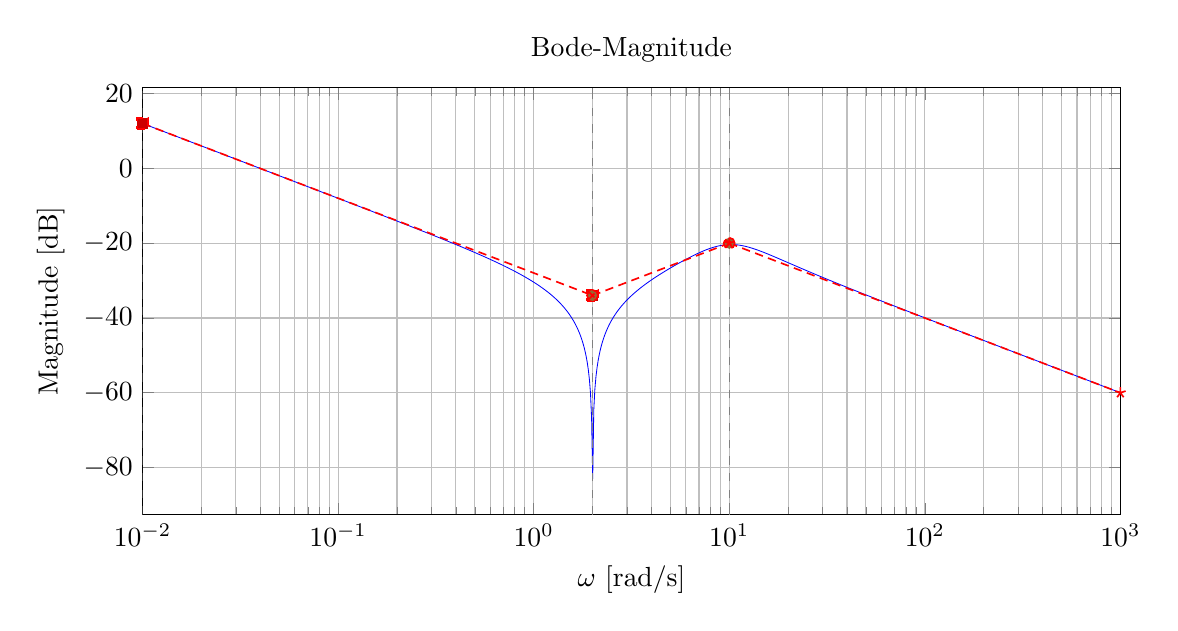
\begin{tikzpicture}
\begin{semilogxaxis}[
  width=14cm,height=7cm,
  xmin=1e-2,xmax=1e3,
  ytick distance=20,
  xlabel={$\omega$ [rad/s]},
  ylabel={Magnitude [dB]},
  grid=both,
  title={Bode-Magnitude}
]
\addplot[
  domain=1e-2:1e3,
  samples=900,
  mark=none,
  line width=0.3pt,
  blue
] {20*ln(abs(4 - x^2))/ln(10) - 20*ln(x)/ln(10) - 10*ln((100 - x^2)^2 + (10*x)^2)/ln(10)};
\addplot+[domain=1e-2:2,samples=2,dashed,dash pattern=on 3pt off 2pt,line width=0.6pt,red] {20*ln(0.04)/ln(10) - 20*ln(x)/ln(10)};
\addplot+[domain=2:1e1,samples=2,dashed,dash pattern=on 3pt off 2pt,line width=0.6pt,red] {-40 + 20*ln(x)/ln(10)};
\addplot+[domain=1e1:1e3,samples=2,dashed,dash pattern=on 3pt off 2pt,line width=0.6pt,red] {-20 - 20*ln(x/10)/ln(10)};
\draw[gray,dashed] (rel axis cs:0,0) -- (rel axis cs:0,1);
\draw[gray,dashed] (axis cs:2,\pgfkeysvalueof{/pgfplots/ymin}) -- (axis cs:2,\pgfkeysvalueof{/pgfplots/ymax});
\draw[gray,dashed] (axis cs:10,\pgfkeysvalueof{/pgfplots/ymin}) -- (axis cs:10,\pgfkeysvalueof{/pgfplots/ymax});
\node[gray,anchor=south east] at (axis cs:2,\pgfkeysvalueof{/pgfplots/ymax}) {\scriptsize Doppelnullstellen $\omega_z=2$ (j-Achse)};
\node[gray,anchor=south east] at (axis cs:10,\pgfkeysvalueof{/pgfplots/ymax}) {\scriptsize Polpaar $\omega_n=10$, $\zeta=0.5$};
\end{semilogxaxis}
\end{tikzpicture}
\vspace{6mm}
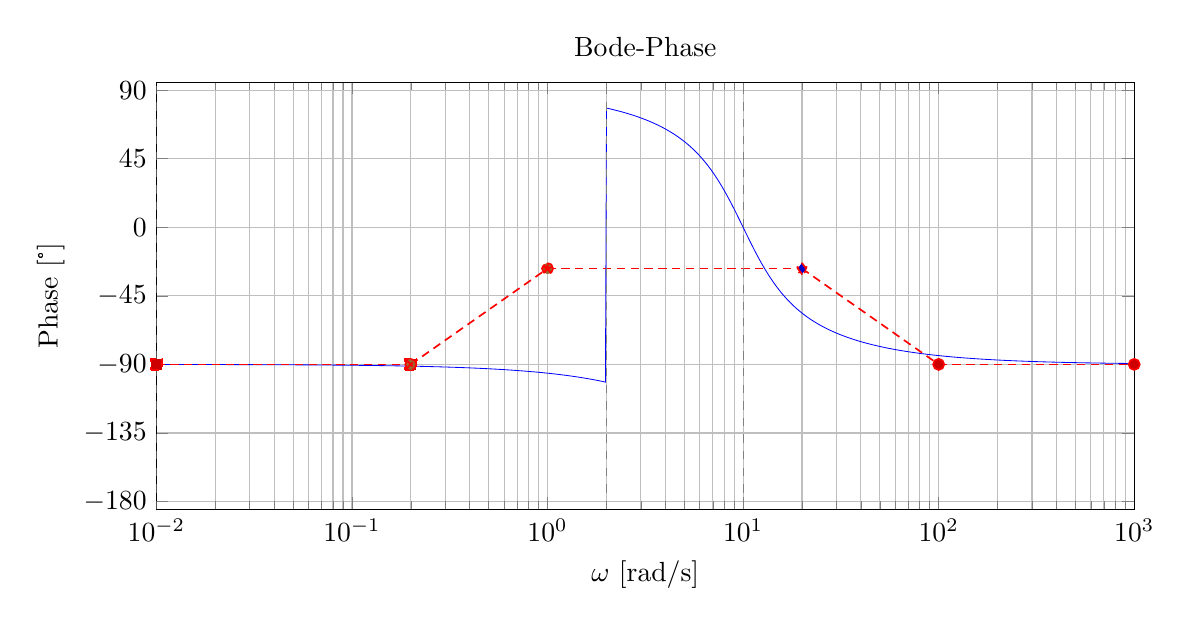
\begin{tikzpicture}
\begin{semilogxaxis}[
  width=14cm,height=7cm,
  xmin=1e-2,xmax=1e3,
  ytick distance=45,
  ymin=-185,ymax=95,
  xlabel={$\omega$ [rad/s]},
  ylabel={Phase [°]},
  grid=both,
  title={Bode-Phase}
]
\addplot[
  domain=1e-2:1e3,
  samples=900,
  mark=none,
  line width=0.3pt,
  blue
] {atan2(0, 4 - x^2) - 90 - atan2(x/10, 1 - (x/10)^2)};
\addplot+[domain=1e-2:2e-1,samples=2,dashed,dash pattern=on 3pt off 2pt,line width=0.6pt,red] {-90};
\addplot+[domain=2e-1:1e0,samples=2,dashed,dash pattern=on 3pt off 2pt,line width=0.6pt,red] {-90 + 90*ln(x/0.2)/ln(10)};
\addplot+[domain=1e0:2e1,samples=2,dashed,dash pattern=on 3pt off 2pt,line width=0.6pt,red] {-90 + 90*ln(5)/ln(10)};
\addplot+[domain=2e1:1e2,samples=2,dashed,dash pattern=on 3pt off 2pt,line width=0.6pt,red] {90 - 90*ln(x)/ln(10)};
\addplot+[domain=1e2:1e3,samples=2,dashed,dash pattern=on 3pt off 2pt,line width=0.6pt,red] {-90};
\draw[gray,dashed] (rel axis cs:0,0) -- (rel axis cs:0,1);
\draw[gray,dashed] (axis cs:2,\pgfkeysvalueof{/pgfplots/ymin}) -- (axis cs:2,\pgfkeysvalueof{/pgfplots/ymax});
\draw[gray,dashed] (axis cs:10,\pgfkeysvalueof{/pgfplots/ymin}) -- (axis cs:10,\pgfkeysvalueof{/pgfplots/ymax});
\node[gray,anchor=south east] at (axis cs:2,\pgfkeysvalueof{/pgfplots/ymax}) {\scriptsize Doppelnullstellen $\omega_z=2$ (j-Achse)};
\node[gray,anchor=south east] at (axis cs:10,\pgfkeysvalueof{/pgfplots/ymax}) {\scriptsize Polpaar $\omega_n=10$, $\zeta=0.5$};
\end{semilogxaxis}
\end{tikzpicture}
\end{center}
\newpage
\subsection{Erklärung}
\vspace{5mm}
\begin{description}[leftmargin=1.2em,labelsep=.6em,font=\bfseries]
\item[Schritt 1] Struktur: Integrator $1/s$, konjugiertes Polpaar mit $\omega_n=10$, $\zeta=0.5$, und Doppelnullen auf der j-Achse bei $\omega_z=2$. Für $\omega\ll2$: $|H(\j\omega)|\approx \dfrac{4}{100\,\omega}=0.04/\omega$ $\Rightarrow$ Slope $-20\,\mathrm{dB/dec}$ um Niveau $20\log_{10}0.04\approx-27.96\,\mathrm{dB}$ bei $\omega=1$; Phase $\approx-90^\circ$.
\item[Schritt 2] Doppelnullen bei $\omega_z=2$: Betrag hat dort ein exaktes Null ($|H(\j2)|=0$). Asymptotisch steigt die Slope hinter $\omega=2$ um $+40\,\mathrm{dB/dec}$ (Netto $-20\to+20\,\mathrm{dB/dec}$). Phasenbeitrag der Zählerdoppelnull ist exakt ein Sprung um $+180^\circ$ (von $0^\circ$ auf $180^\circ$); in der Geradennäherung als $+180^\circ$ über zwei Dekaden $[0.2,20]$ modelliert.
\item[Schritt 3] Polpaar bei $\omega_n=10$, $\zeta=0.5$: ab $\omega=10$ Slope-Änderung $-40\,\mathrm{dB/dec}$ (Netto $+20\to-20\,\mathrm{dB/dec}$). Exakt bei $\omega=10$: $|H(\j10)|=\dfrac{|4-100|}{10\cdot100}=\dfrac{96}{1000}\approx-20.35\,\mathrm{dB}$ (nahe der $-20\,\mathrm{dB}$-Asymptote). Phasenbeitrag des Polpaares $-180^\circ$ über $[1,100]$, wodurch die Gesamtsumme nach dem temporären Anheben durch die Zählernullen wieder gegen $\,-90^\circ$ fällt.
\end{description}

\vspace{0.5cm}
\medskip
\noindent\textbf{Stückweise Näherung}
\[
|H(\j\omega)|_{\mathrm{dB}}\approx
\begin{cases}
20\log_{10}(0.04)-20\log_{10}\omega,& \omega\ll2,\\[4pt]
-\infty,& \omega=2,\\[4pt]
-40+20\log_{10}\omega,& 2\ll\omega\ll10,\\[4pt]
-20-20\log_{10}(\omega/10),& \omega\gg10,
\end{cases}
\qquad
\]
\newpage
\section{}
\[
H(s)=\frac{s^2+2s+10}{s^2+2s+10}=1\,.
\]
\subsection{Bode-Diagramm}
\begin{center}
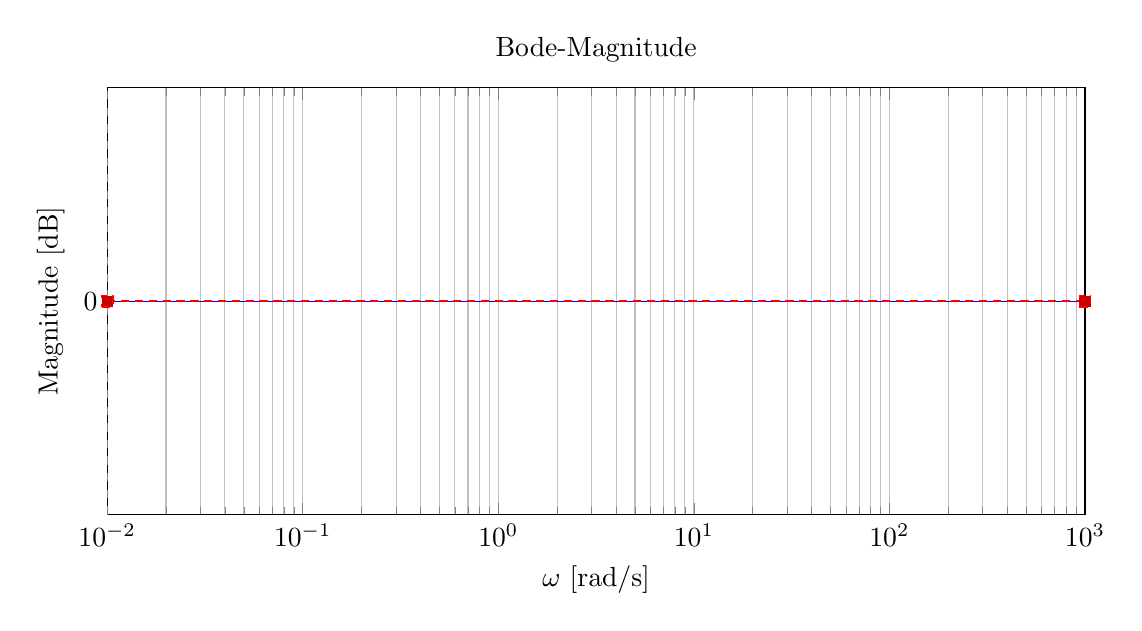
\begin{tikzpicture}
\begin{semilogxaxis}[
  width=14cm,height=7cm,
  xmin=1e-2,xmax=1e3,
  ytick distance=20,
  ytick={-20,0,20},
  xlabel={$\omega$ [rad/s]},
  ylabel={Magnitude [dB]},
  grid=both,
  title={Bode-Magnitude}
]
\addplot[
  domain=1e-2:1e3,
  samples=2,
  mark=none,
  line width=0.3pt,
  blue
] {0};
\addplot+[domain=1e-2:1e3,samples=2,dashed,dash pattern=on 3pt off 2pt,line width=0.6pt,red] {0};
\draw[gray,dashed] (rel axis cs:0,0) -- (rel axis cs:0,1);
\end{semilogxaxis}
\end{tikzpicture}
\vspace{6mm}
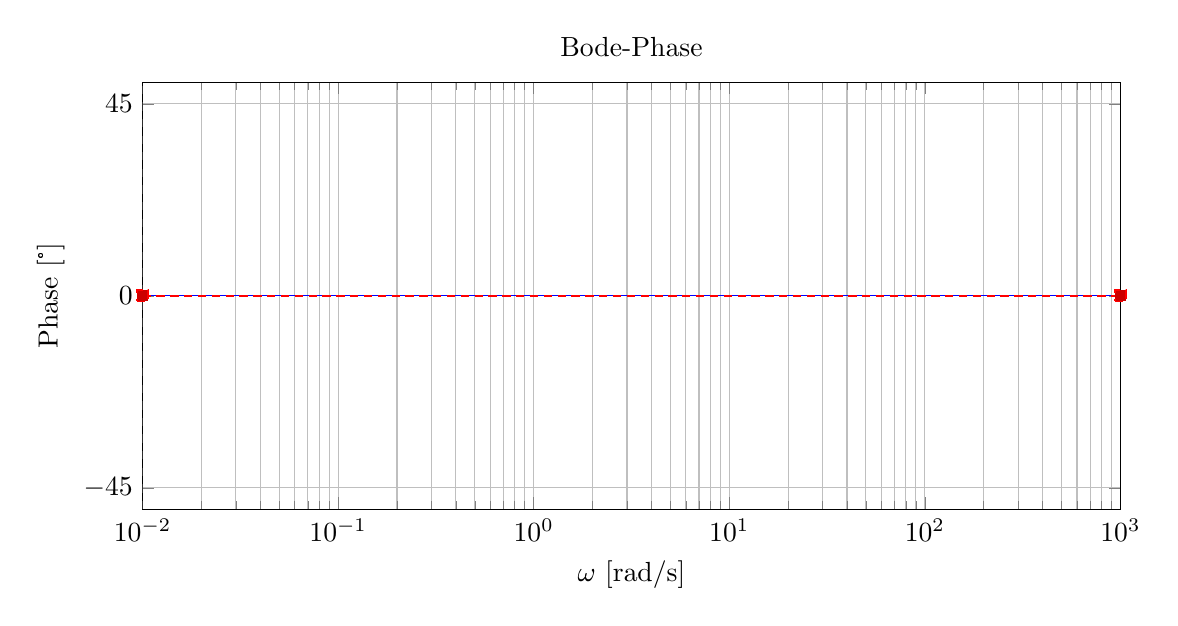
\begin{tikzpicture}
\begin{semilogxaxis}[
  width=14cm,height=7cm,
  xmin=1e-2,xmax=1e3,
  ytick distance=45,
  ymin=-50,ymax=50,
  xlabel={$\omega$ [rad/s]},
  ylabel={Phase [°]},
  grid=both,
  title={Bode-Phase}
]
\addplot[
  domain=1e-2:1e3,
  samples=2,
  mark=none,
  line width=0.3pt,
  blue
] {0};
\addplot+[domain=1e-2:1e3,samples=2,dashed,dash pattern=on 3pt off 2pt,line width=0.6pt,red] {0};
\draw[gray,dashed] (rel axis cs:0,0) -- (rel axis cs:0,1);
\end{semilogxaxis}
\end{tikzpicture}
\end{center}
\newpage
\subsection{Erklärung}
\vspace{5mm}
\begin{description}[leftmargin=1.2em,labelsep=.6em,font=\bfseries]
\item[Schritt 1] Kürzung: Zähler und Nenner sind identisch, daher $H(s)\equiv1$. DC-Faktor $1\Rightarrow |H|_{\mathrm{DC}}=0\,\mathrm{dB}$; Anfangssteigung $0\,\mathrm{dB/dec}$; Phase $0^\circ$.
\item[Schritt 2] Keine Ecken: keine endlichen Pole/Nullstellen nach Kürzung, daher keine Eckfrequenzen und keine Übergangsdekaden. Die Geradennäherungen decken sich exakt mit dem exakten Verlauf.
\item[Schritt 3] Grenzverhalten: für $\omega\to0$ und $\omega\to\infty$ bleibt $|H(\j\omega)|=1$ und $\angle H(\j\omega)=0^\circ$; das gesamte Bode-Diagramm ist konstant.
\end{description}

\vspace{0.5cm}
\medskip
\noindent\textbf{Stückweise Näherung}
\[
|H(\j\omega)|_{\mathrm{dB}}\approx
\begin{cases}
0,& \omega\ll1,\\[4pt]
0,& \omega=1,\\[4pt]
0,& \omega\gg1,
\end{cases}
\qquad
\]
\newpage
\section{}
\[
H(s)=\frac{4}{s^2-4}=\frac{4}{(s-2)(s+2)}\,.
\]
\subsection{Bode-Diagramm}
\begin{center}
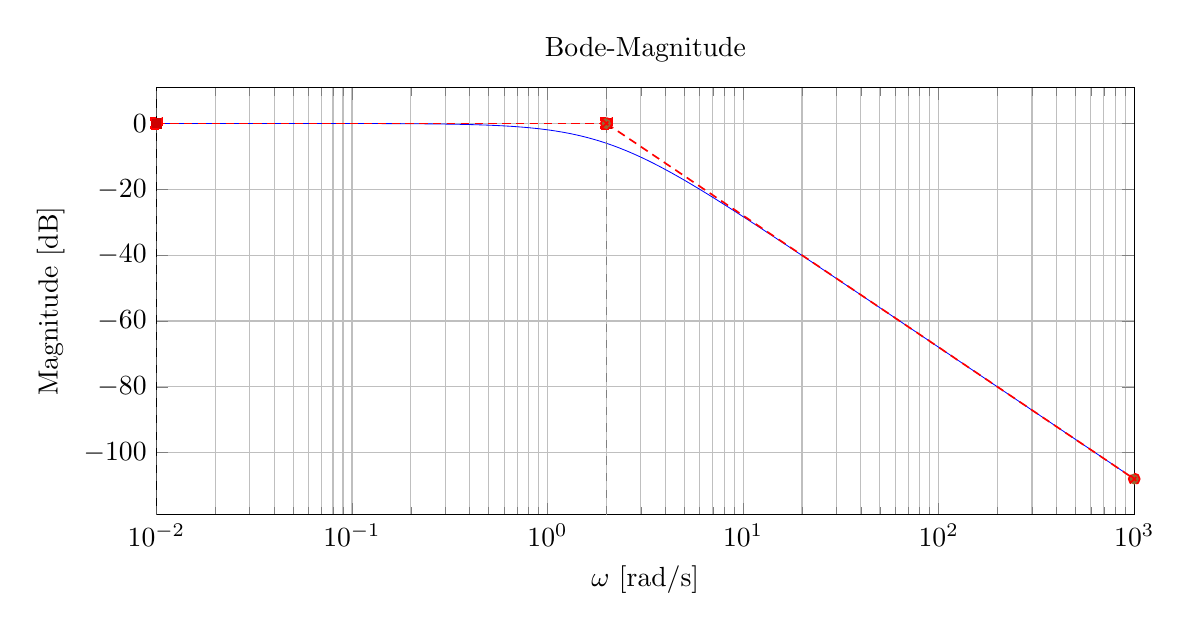
\begin{tikzpicture}
\begin{semilogxaxis}[
  width=14cm,height=7cm,
  xmin=1e-2,xmax=1e3,
  xlabel={$\omega$ [rad/s]},
  ytick distance=20,
  ylabel={Magnitude [dB]},
  grid=both,
  title={Bode-Magnitude}
]
\addplot[
  domain=1e-2:1e3,
  samples=800,
  mark=none,
  line width=0.3pt,
  blue
] {-40*ln(sqrt(1 + (x/2)^2))/ln(10)};
\addplot+[domain=1e-2:2,samples=2,dashed,dash pattern=on 3pt off 2pt,line width=0.6pt,red] {0};
\addplot+[domain=2:1e3,samples=2,dashed,dash pattern=on 3pt off 2pt,line width=0.6pt,red] {-40*ln(x/2)/ln(10)};
\draw[gray,dashed] (rel axis cs:0,0) -- (rel axis cs:0,1);
\draw[gray,dashed] (axis cs:2,\pgfkeysvalueof{/pgfplots/ymin}) -- (axis cs:2,\pgfkeysvalueof{/pgfplots/ymax});
\node[gray,anchor=south east] at (axis cs:2,\pgfkeysvalueof{/pgfplots/ymax}) {\scriptsize Pole $\omega_p=2$ (LHP \& RHP)};
\end{semilogxaxis}
\end{tikzpicture}
\vspace{6mm}
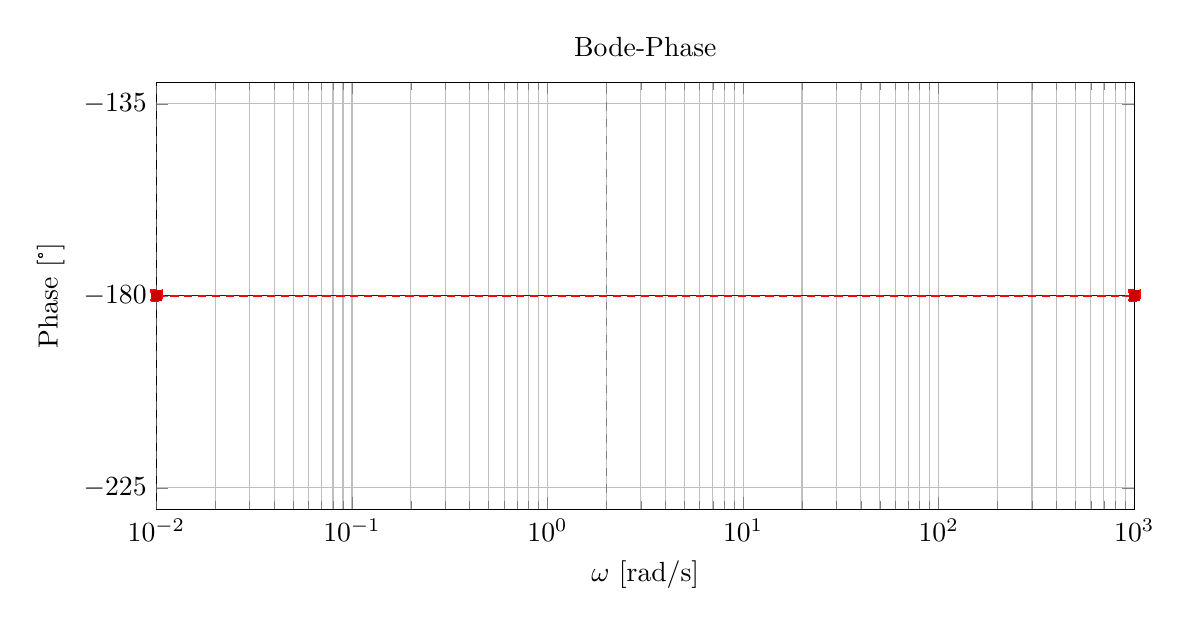
\begin{tikzpicture}
\begin{semilogxaxis}[
  width=14cm,height=7cm,
  xmin=1e-2,xmax=1e3,
  ymin=-230,ymax=-130,
  ytick distance = 45,
  xlabel={$\omega$ [rad/s]},
  ylabel={Phase [°]},
  grid=both,
  title={Bode-Phase}
]
\addplot[
  domain=1e-2:1e3,
  samples=2,
  mark=none,
  line width=0.3pt,
  blue
] {-180};
\addplot+[domain=1e-2:1e3,samples=2,dashed,dash pattern=on 3pt off 2pt,line width=0.6pt,red] {-180};
\draw[gray,dashed] (rel axis cs:0,0) -- (rel axis cs:0,1);
\draw[gray,dashed] (axis cs:2,\pgfkeysvalueof{/pgfplots/ymin}) -- (axis cs:2,\pgfkeysvalueof{/pgfplots/ymax});
\node[gray,anchor=south east] at (axis cs:2,\pgfkeysvalueof{/pgfplots/ymax}) {\scriptsize Pole $\omega_p=2$ (LHP \& RHP)};
\end{semilogxaxis}
\end{tikzpicture}
\end{center}
\newpage
\subsection{Erklärung (ausführlich)}
\begin{description}[leftmargin=1.2em,labelsep=.6em,font=\bfseries]

\item[1. Normalform herstellen.]
\[
H(s)=\frac{4}{(s-2)(s+2)}
= K_0\cdot\frac{1}{(1-sT_{p1})}\cdot\frac{1}{(1+sT_{p2})}
\]
mit
\[
K_0=-1,\quad r=0,\quad T_{p1}=\tfrac{1}{2},\quad T_{p2}=\tfrac{1}{2}.
\]

\item[2. Eckfrequenz bestimmen und sortieren.]
\[
\omega_{p1}=\tfrac{1}{T_{p1}}=\omega_{p2}=\tfrac{1}{T_{p2}}=2\,\mathrm{rad/s}
\]

\item[3. Startpunkt des Amplitudengangs festlegen.]
Setze \(\omega_{\min}=\omega_p=2\).
\[
F_{\mathrm{dB}}(\omega_{\min})=20\log_{10}\!\big(|K_0\,\underline{F}^*_{\mathrm{ges}}(0)|\,\omega_{\min}^{\,r}\big)
=20\log_{10}(1)=0\,\mathrm{dB}.
\]
Ankerpunkt: \(0\,\mathrm{dB}\) bei \(\omega=2\).

\item[4. Verlauf links vom Startpunkt zeichnen.]
Für \(\omega<2\): Anfangssteigung \(r\cdot 20=0\,\mathrm{dB/dec}\) \(\Rightarrow\) horizontale Asymptote bei \(0\,\mathrm{dB}\).

\item[5. Steigungswechsel an der Eckfrequenz eintragen.]
Ab \(\omega=2\): zwei einfache Pole (RHP \& LHP) \(\Rightarrow\) zusätzliche \(-40\,\mathrm{dB/dec}\). Netto:
\[
\begin{cases}
0\,\mathrm{dB},& \omega<2,\\
-40\log_{10}(\omega/2),& \omega\ge 2.
\end{cases}
\]

\item[6. Eckabrundung korrekt berücksichtigen.]
Am Knick \(\omega=2\): Summe zweier \(-3\,\mathrm{dB}\)\ \(\Rightarrow\)\ \(-6\,\mathrm{dB}\) unter der Geraden:
\[
|H(j2)|_{\mathrm{dB}}\approx -6\,\mathrm{dB}.
\]
(Dies gilt hier trotz RHP/LHP-Mischung, da es um den \emph{Betrag} geht.)

\item[7. Phasenstartwert festlegen.]
Da \(K_0\,\underline{F}^*_{\mathrm{ges}}(0)<0\) und \(r=0\),
\[
\varphi(0)=-180^\circ + r\cdot90^\circ = -180^\circ.
\]

\item[8. Phasenänderung durch die Polglieder (Überlappung/Kompensation).]
Ein LHP-Pol trägt \(-90^\circ\) über seine Übergangsdekade \([0.2,20]\) bei, ein RHP-Pol gleicher Lage trägt \(+90^\circ\) über \([0.2,20]\) bei. Diese Beiträge überlappen vollständig und kompensieren sich zu \(0^\circ\); daher bleibt die Phase für alle \(\omega\) konstant bei \(-180^\circ\) (der durch \(K_0<0\) vorgegebene Offset).

\item[9. Grenzwerte und Konsistenz prüfen.]
DC: \(|H(0)|=1\Rightarrow 0\,\mathrm{dB}\), \(\varphi(0)=-180^\circ\).
HF: \(|H(j\omega)|=\frac{4}{\omega^2+4}\sim \frac{4}{\omega^2}\Rightarrow -40\log_{10}(\omega/2)\,\mathrm{dB}\), \(\varphi(\infty)=-180^\circ\).

\end{description}

\subsubsection*{Stückweise Näherungen (für die Skizze)}
\[
|H(j\omega)|_{\mathrm{dB}}\approx
\begin{cases}
0,& \omega\ll 2,\\[2pt]
-6,& \omega=2,\\[2pt]
-40\log_{10}(\omega/2),& \omega\gg 2,
\end{cases}
\]
\[
\varphi(\omega)\approx
\begin{cases}
-180^\circ,& \text{für alle }\omega.
\end{cases}
\]

\newpage
\section{}
\[
H(s)=\frac{-1000\,(s+2)^2}{4\,(s+1)^3\,(s+10)}=-250\,\frac{(s+2)^2}{(s+1)^3\,(s+10)}\,.
\]
\subsection{Bode-Diagramm}
\begin{center}
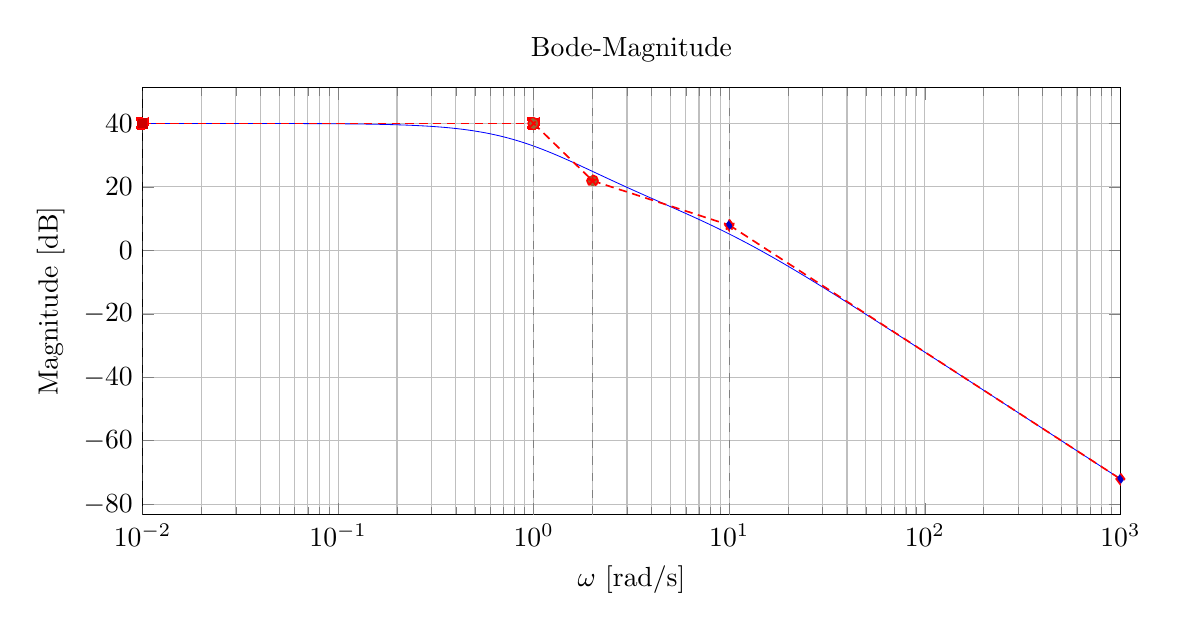
\begin{tikzpicture}
\begin{semilogxaxis}[
  width=14cm,height=7cm,
  ytick distance=20,
  xmin=1e-2,xmax=1e3,
  xlabel={$\omega$ [rad/s]},
  ylabel={Magnitude [dB]},
  grid=both,
  title={Bode-Magnitude}
]
\addplot[
  domain=1e-2:1e3,
  samples=900,
  mark=none,
  line width=0.3pt,
  blue
] {20*ln(250)/ln(10)
    +40*ln(sqrt(4 + x^2))/ln(10)
    -60*ln(sqrt(1 + x^2))/ln(10)
    -20*ln(sqrt(100 + x^2))/ln(10)};
\addplot+[domain=1e-2:1,samples=2,dashed,dash pattern=on 3pt off 2pt,line width=0.6pt,red] {40};
\addplot+[domain=1:2,samples=2,dashed,dash pattern=on 3pt off 2pt,line width=0.6pt,red] {40 - 60*ln(x)/ln(10)};
\addplot+[domain=2:1e1,samples=2,dashed,dash pattern=on 3pt off 2pt,line width=0.6pt,red] {40 - 60*ln(2)/ln(10) - 20*ln(x/2)/ln(10)};
\addplot+[domain=1e1:1e3,samples=2,dashed,dash pattern=on 3pt off 2pt,line width=0.6pt,red] {40 - 60*ln(2)/ln(10) - 20*ln(10/2)/ln(10) - 40*ln(x/10)/ln(10)};
\draw[gray,dashed] (rel axis cs:0,0) -- (rel axis cs:0,1);
\draw[gray,dashed] (axis cs:1,\pgfkeysvalueof{/pgfplots/ymin}) -- (axis cs:1,\pgfkeysvalueof{/pgfplots/ymax});
\draw[gray,dashed] (axis cs:2,\pgfkeysvalueof{/pgfplots/ymin}) -- (axis cs:2,\pgfkeysvalueof{/pgfplots/ymax});
\draw[gray,dashed] (axis cs:10,\pgfkeysvalueof{/pgfplots/ymin}) -- (axis cs:10,\pgfkeysvalueof{/pgfplots/ymax});
\node[gray,anchor=south east] at (axis cs:2,\pgfkeysvalueof{/pgfplots/ymax}) {\scriptsize Nullstelle $\omega_z=2$ (doppelt)};
\node[gray,anchor=south east] at (axis cs:1,\pgfkeysvalueof{/pgfplots/ymax}) {\scriptsize Pol $\omega_p=1$ (dreifach)};
\node[gray,anchor=south east] at (axis cs:10,\pgfkeysvalueof{/pgfplots/ymax}) {\scriptsize Pol $\omega_p=10$};
\end{semilogxaxis}
\end{tikzpicture}
\vspace{6mm}
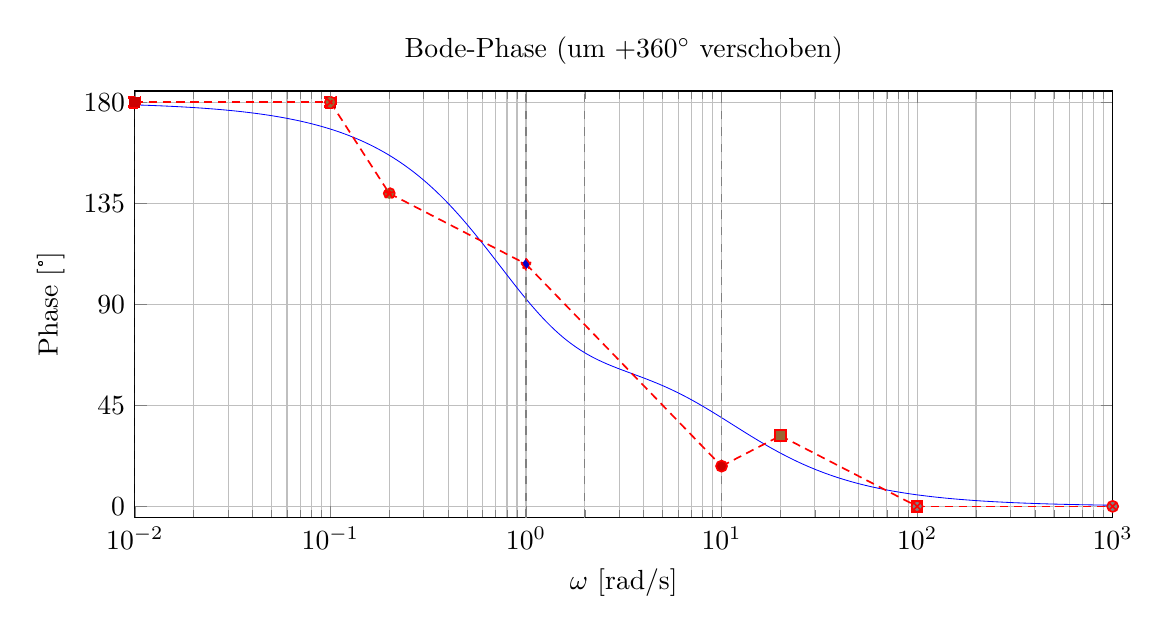
\begin{tikzpicture}
\begin{semilogxaxis}[
  width=14cm,height=7cm,
  xmin=1e-2,xmax=1e3,
  ymin=-5,ymax=185,
  ytick distance=45,
  xlabel={$\omega$ [rad/s]},
  ylabel={Phase [°]},
  grid=both,
  title={Bode-Phase (um $+360^\circ$ verschoben)}
]
% exakte (blaue) Phase: +360° Shift
\addplot[
  domain=1e-2:1e3,
  samples=900,
  mark=none,
  line width=0.3pt,
  blue
] {180 + 2*atan(x/2) - 3*atan(x) - atan(x/10)};

% rote Geradennäherung, korrekt platziert und +360° verschoben
\addplot+[domain=1e-2:1e-1,samples=2,dashed,dash pattern=on 3pt off 2pt,line width=0.6pt,red]{180};
\addplot+[domain=1e-1:2e-1,samples=2,dashed,dash pattern=on 3pt off 2pt,line width=0.6pt,red]{180 - 135*ln(x/0.1)/ln(10)};
\addplot+[domain=2e-1:1e0,samples=2,dashed,dash pattern=on 3pt off 2pt,line width=0.6pt,red]{180 - 135*ln(2)/ln(10) - 45*ln(x/0.2)/ln(10)};
\addplot+[domain=1e0:1e1,samples=2,dashed,dash pattern=on 3pt off 2pt,line width=0.6pt,red]{180 - 135*ln(2)/ln(10) - 45*ln(5)/ln(10) - 90*ln(x)/ln(10)};
\addplot+[domain=1e1:2e1,samples=2,dashed,dash pattern=on 3pt off 2pt,line width=0.6pt,red]{180 - 135*ln(2)/ln(10) - 45*ln(5)/ln(10) - 90 + 45*ln(x/10)/ln(10)};
\addplot+[domain=2e1:1e2,samples=2,dashed,dash pattern=on 3pt off 2pt,line width=0.6pt,red]{180 - 135*ln(2)/ln(10) - 45*ln(5)/ln(10) - 90 + 45*ln(2)/ln(10) - 45*ln(x/20)/ln(10)};
\addplot+[domain=1e2:1e3,samples=2,dashed,dash pattern=on 3pt off 2pt,line width=0.6pt,red]{0};

\draw[gray,dashed] (rel axis cs:0,0) -- (rel axis cs:0,1);
\draw[gray,dashed] (axis cs:1,\pgfkeysvalueof{/pgfplots/ymin}) -- (axis cs:1,\pgfkeysvalueof{/pgfplots/ymax});
\draw[gray,dashed] (axis cs:2,\pgfkeysvalueof{/pgfplots/ymin}) -- (axis cs:2,\pgfkeysvalueof{/pgfplots/ymax});
\draw[gray,dashed] (axis cs:10,\pgfkeysvalueof{/pgfplots/ymin}) -- (axis cs:10,\pgfkeysvalueof{/pgfplots/ymax});
\node[gray,anchor=south east] at (axis cs:2,\pgfkeysvalueof{/pgfplots/ymax}) {\scriptsize Nullstelle $\omega_z=2$ (doppelt)};
\node[gray,anchor=south east] at (axis cs:1,\pgfkeysvalueof{/pgfplots/ymax}) {\scriptsize Pol $\omega_p=1$ (dreifach)};
\node[gray,anchor=south east] at (axis cs:10,\pgfkeysvalueof{/pgfplots/ymax}) {\scriptsize Pol $\omega_p=10$};
\end{semilogxaxis}
\end{tikzpicture}
\end{center}
\newpage

\subsection{Erklärung}
\vspace{5mm}
\begin{description}[leftmargin=1.2em,labelsep=.6em,font=\bfseries]
\item[Schritt 1] Konstante \& Vorzeichen: $H(0)=-100\Rightarrow |H|_{\mathrm{DC}}=40\,\mathrm{dB}$, Anfangssteigung $0\,\mathrm{dB/dec}$. Die Darstellung ist um $+360^\circ$ verschoben: Startphase $180^\circ$ (das negative Vorzeichen).
\item[Schritt 2] Dreifachpol bei $\omega=1\,\mathrm{rad/s}$: ab $\omega=1$ Steigungsänderung um $-60\,\mathrm{dB/dec}$; Exakte Abweichung ggü. Geradennäherung $-3\cdot10\log_{10}2\approx-9\,\mathrm{dB}$. Phasenabfall dieses Poltripels über $\omega\in[0.1,10]$ um $270^\circ$.
\item[Schritt 3] Doppelnullstelle bei $\omega=2\,\mathrm{rad/s}$ und Pol bei $\omega=10\,\mathrm{rad/s}$: die Doppelnull hebt die Slope ab $\omega=2$ um $+40\,\mathrm{dB/dec}$ (Netto $-20\,\mathrm{dB/dec}$ in $(2,10)$), der Pol bei $\omega=10$ senkt sie um weitere $-20\,\mathrm{dB/dec}$ (Netto $-40\,\mathrm{dB/dec}$ für $\omega\gg10$). Phasenbeiträge: $+180^\circ$ der Doppelnullstelle über $[0.2,20]$, $-90^\circ$ des Pols bei $10$ über $[1,100]$; Die Phase verläuft von $180^\circ$ ($\omega \ll 0.1$) gegen $0^\circ$ ($100 \ll \omega$).
\end{description}

\vspace{0.5cm}
\medskip
\noindent\textbf{Stückweise Näherung}
\[
|H(\j\omega)|_{\mathrm{dB}}\approx
\begin{cases}
40,& \omega\ll1,\\[4pt]
40-60\log_{10}\omega,& 1\ll\omega\ll2,\\[4pt]
40-60\log_{10}2-20\log_{10}(\omega/2),& 2\ll\omega\ll10,\\[4pt]
40-60\log_{10}2-20\log_{10}5-40\log_{10}(\omega/10),& \omega\gg10,
\end{cases}
\qquad
\]
\newpage
\section{}
\[
H(s)=\frac{2\,s}{s^2+2s+1}=\frac{2\,s}{(s+1)^2}\,.
\]
\subsection{Bode-Diagramm}
\begin{center}
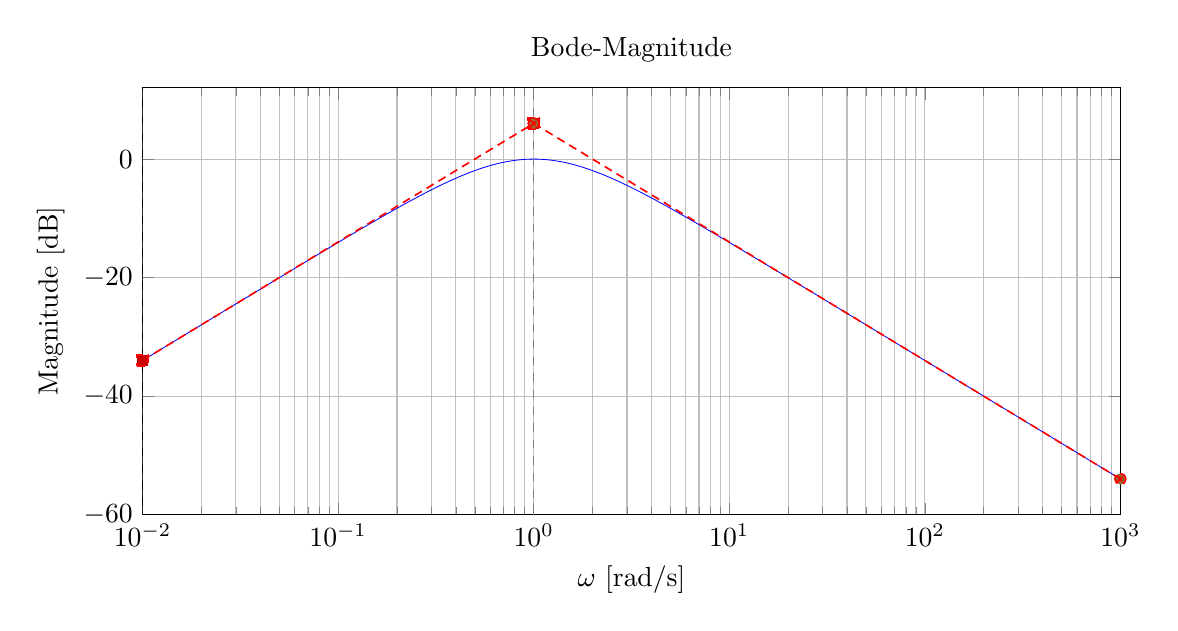
\begin{tikzpicture}
\begin{semilogxaxis}[
  width=14cm,height=7cm,
  xmin=1e-2,xmax=1e3,
  ytick distance=20,
  xlabel={$\omega$ [rad/s]},
  ylabel={Magnitude [dB]},
  grid=both,
  title={Bode-Magnitude}
]
\addplot[
  domain=1e-2:1e3,
  samples=700,
  mark=none,
  line width=0.3pt,
  blue
] {20*ln(2)/ln(10) + 20*ln(x)/ln(10) - 40*ln(sqrt(1 + x^2))/ln(10)};
\addplot+[domain=1e-2:1,samples=2,dashed,dash pattern=on 3pt off 2pt,line width=0.6pt,red] {20*ln(2)/ln(10) + 20*ln(x)/ln(10)};
\addplot+[domain=1:1e3,samples=2,dashed,dash pattern=on 3pt off 2pt,line width=0.6pt,red] {20*ln(2)/ln(10) - 20*ln(x)/ln(10)};
\draw[gray,dashed] (rel axis cs:0,0) -- (rel axis cs:0,1);
\draw[gray,dashed] (axis cs:1,\pgfkeysvalueof{/pgfplots/ymin}) -- (axis cs:1,\pgfkeysvalueof{/pgfplots/ymax});
\node[gray,anchor=south east] at (axis cs:1,\pgfkeysvalueof{/pgfplots/ymax}) {\scriptsize Pol $\omega_p=1$ (doppelt)};
\node[gray,anchor=south east] at (axis cs:1e-2,\pgfkeysvalueof{/pgfplots/ymax}) {\scriptsize Nullstelle im Ursprung};
\end{semilogxaxis}
\end{tikzpicture}
\vspace{6mm}
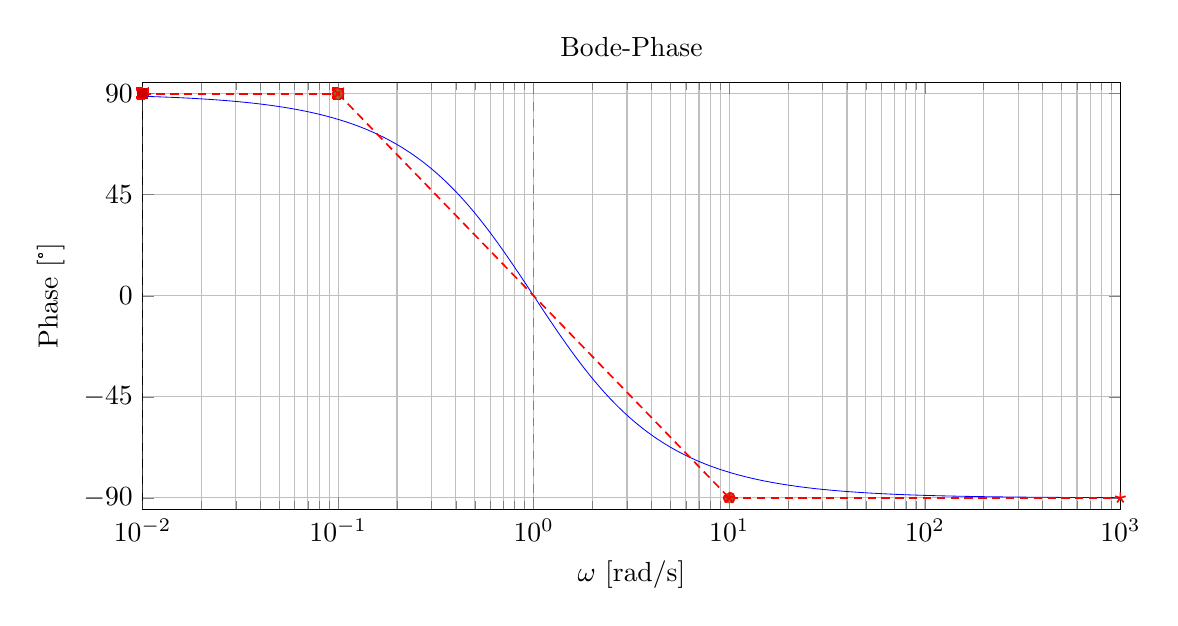
\begin{tikzpicture}
\begin{semilogxaxis}[
  width=14cm,height=7cm,
  xmin=1e-2,xmax=1e3,
  ymin=-95,ymax=95,
  ytick distance=45,
  xlabel={$\omega$ [rad/s]},
  ylabel={Phase [°]},
  grid=both,
  title={Bode-Phase}
]
\addplot[
  domain=1e-2:1e3,
  samples=700,
  mark=none,
  line width=0.3pt,
  blue
] {90 - 2*atan(x)};
\addplot+[domain=1e-2:1e-1,samples=2,dashed,dash pattern=on 3pt off 2pt,line width=0.6pt,red] {90};
\addplot+[domain=1e-1:1e1,samples=2,dashed,dash pattern=on 3pt off 2pt,line width=0.6pt,red] {45 - 90*ln(x)/ln(10) - 45};
\addplot+[domain=1e1:1e3,samples=2,dashed,dash pattern=on 3pt off 2pt,line width=0.6pt,red] {-90};
\draw[gray,dashed] (rel axis cs:0,0) -- (rel axis cs:0,1);
\draw[gray,dashed] (axis cs:1,\pgfkeysvalueof{/pgfplots/ymin}) -- (axis cs:1,\pgfkeysvalueof{/pgfplots/ymax});
\node[gray,anchor=south east] at (axis cs:1,\pgfkeysvalueof{/pgfplots/ymax}) {\scriptsize Pol $\omega_p=1$ (doppelt)};
\node[gray,anchor=south east] at (axis cs:1e-2,\pgfkeysvalueof{/pgfplots/ymax}) {\scriptsize Nullstelle im Ursprung};
\end{semilogxaxis}
\end{tikzpicture}
\end{center}
\newpage
\subsection{Erklärung (ausführlich)}
\begin{description}[leftmargin=1.2em,labelsep=.6em,font=\bfseries]

\item[1. Normalform herstellen.]
\[
H(s)=\frac{2s}{(s+1)^2}
=K_0\cdot s^{\,r}\cdot \frac{1}{(1+sT_p)^2}
\]
mit
\[
K_0=2,\quad r=1\ (\text{Nullstelle im Ursprung}),\quad T_p=1\ (\text{Doppelpol bei } \omega_p=1).
\]
Teilglieder:  \(\underline{F}_1(s)=\frac{1}{(1+s)^2}\) (reelles Polglied 2. Ordnung).

\item[2. Eckfrequenz bestimmen und sortieren.]
\[
\omega_p=\frac{1}{T_p}=1\,\mathrm{rad/s}.
\]
Nur diese Eckfrequenz; Sortierung trivial.

\item[3. Startpunkt des Amplitudengangs festlegen (Geradennäherung).]
Setze \(\omega_{\min}=\omega_p=1\). Skript-Regel:
\[
F_{\mathrm{dB}}(\omega_{\min})=20\log_{10}\!\big(|K_0\,\underline{F}_{ges}^*(0)|\cdot \omega_{\min}^{\,r}\big)
=20\log_{10}(2\cdot 1\cdot 1)=20\log_{10}2\approx +6\,\mathrm{dB}.
\]
Ankerpunkt der Geraden: \(+6\,\mathrm{dB}\) bei \(\omega=1\).

\item[4. Verlauf links vom Startpunkt zeichnen.]
Für \(\omega<1\) gilt Anfangssteigung \(r\cdot 20\,\mathrm{dB/dec}=+20\,\mathrm{dB/dec}\) (Nullstelle im Ursprung). Zeichne links vom Ankerpunkt eine Gerade mit \(+20\,\mathrm{dB/dec}\).

\item[5. Steigungswechsel an der Eckfrequenz eintragen.]
Doppelpol bei \(\omega=1\) bewirkt \(-40\,\mathrm{dB/dec}\) ab \(\omega=1\). Netto-Steigung:
\[
\begin{cases}
+20\,\mathrm{dB/dec},& \omega<1,\\
-20\,\mathrm{dB/dec},& \omega>1
\end{cases}
\]
(d.\,h.\ zwischen \(1\) und \(\infty\) fällt die Gerade mit \(-20\,\mathrm{dB/dec}\)).

\item[6. Eckabrundung korrekt berücksichtigen.]
Am Knick eines Doppelpols: \(-6\,\mathrm{dB}\) unter der Geradennäherung.
\[
|H(\j1)|_{\mathrm{dB}}\approx \underbrace{20\log_{10}2}_{\approx+6}\;-\;6=0\,\mathrm{dB}.
\]

\item[7. Phasenstartwert festlegen.]
Regel mit Vorzeichen und Ursprungsnull:
\[
K_0\,\underline{F}_{ges}^*(0)>0,\quad r=1
\;\Rightarrow\;
\varphi(0)=r\cdot 90^\circ=1\cdot 90^\circ=+90^\circ.
\]

\item[8. Phasenänderung durch Nullstelle und Doppelpol eintragen.]
Die Nullstelle im Ursprung liefert einen \emph{konstanten} Offset von \(+90^\circ\). Der Doppelpol bewirkt \(-180^\circ\) über die zwei Dekaden \([0.1,10]\) (je Pol \(-90^\circ\)). 
\textbf{Überlappung/Addierung:} In der Übergangszone \([0.1,10]\) wirken beide Polbeiträge gleichzeitig und addieren ihre Steigungen (insgesamt \(-90^\circ/\text{dec}\)). Der Offset \(+90^\circ\) der Ursprungsnull bleibt währenddessen konstant. Damit fällt die Phase von \(+90^\circ\) (für \(\omega\ll0.1\)) über \(0^\circ\) (bei \(\omega\approx1\)) weiter auf \(-90^\circ\) (für \(\omega\gg10\)). Näherung:
\[
\varphi(\omega)\approx
\begin{cases}
+90^\circ,& \omega\le 0.1,\\[2pt]
\;\;0^\circ-90^\circ\log_{10}\omega,& 0.1<\omega<10,\\[2pt]
-90^\circ,& \omega\ge 10.
\end{cases}
\]

\item[9. Grenzwerte und Konsistenz prüfen.]
DC: \(|H(0)|=0\Rightarrow -\infty\,\mathrm{dB}\), \(\varphi(0)=+90^\circ\).
HF: \(|H(\j\omega)|\sim 2/\omega\Rightarrow 20\log_{10}2-20\log_{10}\omega\,\mathrm{dB}\), \(\varphi(\infty)=(r-2)\cdot90^\circ=(1-2)\cdot90^\circ=-90^\circ\) (Pol-/Nullzählung konsistent).

\end{description}

\subsubsection*{Stückweise Näherungen (für die Skizze)}
\[
|H(j\omega)|_{\mathrm{dB}}\approx
\begin{cases}
20\log_{10}2+20\log_{10}\omega,& \omega\ll 1,\\[2pt]
\bigl(20\log_{10}2\bigr)-6=0,& \omega=1,\\[2pt]
20\log_{10}2-20\log_{10}\omega,& \omega\gg 1,
\end{cases}
\]\[
\varphi(\omega)\approx
\begin{cases}
+90^\circ,& \omega\le 0.1,\\[2pt]
0^\circ-90^\circ\log_{10}\omega,& 0.1<\omega<10,\\[2pt]
-90^\circ,& \omega\ge 10.
\end{cases}
\]
\newpage
\end{document}